\documentclass[acmlarge]{acmart}

\usepackage[ruled]{algorithm2e} % For algorithms
\usepackage{balance}       % to better equalize the last page
\usepackage{graphics}      % for EPS, load graphicx instead
%\usepackage[T1]{fontenc}   % for umlauts and other diaeresis
%\usepackage{txfonts}    % this package makes the symbol "=" and "+" undisplayed.
%\usepackage{mathptmx}
\usepackage{amsmath}
%\usepackage{textcomp}
%\usepackage{booktabs}
\usepackage{colortbl}
%\usepackage{microtype}        % Improved Tracking and Kerning
\usepackage{ccicons}          % Cite your images correctly!
%\usepackage{mathrsfs}
\usepackage{subfigure}
\usepackage{multirow}
\usepackage{xspace}
\usepackage{enumitem}
\usepackage{rotating}
\usepackage{caption}
\usepackage{color}
\usepackage{epsf}
\usepackage{times}
\usepackage{epsfig}
\usepackage{url}
%\usepackage{amssymb}
%\usepackage{amsxtra}
%\usepackage{listings}
%\usepackage{verbatim}
\usepackage{pseudocode}
\usepackage{epstopdf}
\usepackage{ifpdf}
\usepackage{subfigure}
%\usepackage{balance}
\usepackage{booktabs}
%\usepackage{multirow}
%\usepackage{array}
%\usepackage{makecell}
%\usepackage{slashbox}
\usepackage{tabularx}
\usepackage{diagbox}
\usepackage{color,soul}

\renewcommand{\algorithmcfname}{ALGORITHM}
\newtheorem{theorem}{Theorem}
\newcommand{\systemname}{\textsc{SleepGuard}\xspace}

\renewcommand{\textrightarrow}{$\rightarrow$}

\newcommand{\red}[1]{\textcolor{red}{#1}}
\newcommand{\blue}[1]{\textcolor{blue}{#1}}
\newcommand{\yellow}[1]{\textcolor{yellow}{#1}}
\newcommand{\green}[1]{\textcolor{green}{#1}}
\newcommand{\cyan}[1]{\textcolor{cyan}{#1}}
\newcommand{\brown}[1]{\textcolor{brown}{#1}}
\newcommand{\purple}[1]{\textcolor{purple}{#1}}
\newcommand{\orange}[1]{\textcolor{orange}{#1}}
\definecolor{Gray}{gray}{0.9}

\newcommand{\etal}{\emph{et al.}}
\newcommand\FIXME[1]{\textcolor{red}{FIX:}\textcolor{red}{#1}}


\SetAlFnt{\small} \SetAlCapFnt{\small} \SetAlCapNameFnt{\small} \SetAlCapHSkip{0pt} \IncMargin{-\parindent}

% Metadata Information
\acmJournal{IMWUT} \acmVolume{9} \acmNumber{4} \acmArticle{39} \acmYear{2018} \acmMonth{2} \acmArticleSeq{11}
% Copyright
\setcopyright{acmcopyright}
%\setcopyright{acmlicensed}
%\setcopyright{rightsretained}
%\setcopyright{usgov}
\setcopyright{usgovmixed}
%\setcopyright{cagov}
%\setcopyright{cagovmixed}
\acmPrice{15.00}

% DOI
\acmDOI{0000001.0000001}
% Paper history
%\received{February 2018} \received{March 2018} \received[accepted]{June 2018}


\begin{document}

\title{\systemname: Capturing Rich Sleep Information using Smartwatch Sensing Data}

%\author{Liqiong Chang, Jiaqi Lu, Ju Wang, Xiaojiang Chen, Dingyi Fang, Zhanyong Tang}
%\orcid{1234-5678-9012-3456}
%\affiliation{
%	\institution{Northwest University}
%	\country{China}} \email{{changliqiong, jqlu, xjchen, dyf, zytang}@nwu.edu.cn}
%
%\author{Petteri Nurmi, Zheng Wang}
%\affiliation{
%	\institution{Lancaster University}
%	\country{United Kingdom}} \email{{p.nurmi, z.wang}@lancaster.ac.uk}

%NOTE: This is supposed to be anonymous review.

\begin{abstract}
Sleep is an important part of our daily routine -- we spend about one-third of our time doing it. By tracking the sleep-related events
and activities, sleep monitoring provides the decision support to help us understand the sleep quality and the causes of poor sleep.
Wearable devices provide a new way for sleep monitoring, allowing us to monitor sleep from the comfort of our own home, but existing
solutions do not take full advantage of the rich sensor data provided by these portable devices. In this paper, we develop a novel
approach to track a wide range of sleep-related events using smartwatches. We show that it is possible to track, using a single
smartwatch, sleep events like body postures and movements, acoustic events, and illumination conditions. From these events, a statistical
model can be designed to effectively evaluate a user's sleep quality across various sleep stages. We evaluate our approach by conducting
extensive experiments involved fifteen users across a 2-week period. Our experimental results show that our approach can track a richer
set of sleep events, which provides better decision support for evaluating the sleep quality, when compared to prior work. We show that
\systemname successfully helps some of our testing users to improve their sleep quality by understanding the causes of poor sleeps. 
\end{abstract}


\begin{CCSXML}
	<ccs2012>
	<concept>
	<concept_id>10003120.10003138</concept_id>
	<concept_desc>Human-centered computing~Ubiquitous and mobile computing</concept_desc>
	<concept_significance>500</concept_significance>
	</concept>
	</ccs2012>
\end{CCSXML}

\ccsdesc[500]{Human-centered computing~Ubiquitous and mobile computing}

\keywords{Smartwatch, Sleep events, Sensing}


\maketitle




\section{INTRODUCTION}\label{sec:1introduction}

Sleep plays a vital role in good health and personal well-being throughout one's life. Lack of sleep or poor quality of sleep can lead to
serious, sometimes life-threatening, health problems~\cite{altena2008sleep,chandola2010effect,lallukka2016contribution}, decrease level of
cognitive performance~\cite{alhola07sleep,akerstedt07altered}, and affect mood and feelings of personal
well-being~\cite{paunio09longitudinal,pilcher97sleep}. Besides having an adverse effect on individuals, insufficient or poor quality sleep
has a significant economic burden, among others, through decreased productivity, and medical and social costs associated with treatment of
sleep disorders~\cite{hafner17why}. Indeed, to highlight the significance of sleep quality, the Centre for Disease Prevention (CDC) has
declared insufficient sleep as a public health problem in the US~\cite{sleepreport}, and the concern is widely shared amongst other
industrialized countries.

Traditionally, sleep monitoring is performed in a clinical environment using Polysomnography (PSG). In PSG, medical sensors attached to human body are used to monitor events and information such as respiration, electroencephalogram (EEG), electrocardiogram (ECG), electro-oculogram and oxygen saturation~\cite{ebrahimi2008automatic,saper2005hypothalamic,oropesa1999sleep,langkvist2012sleep}. These information sources can then be used to determine
sleep stages, sleep efficiency, abnormal breathing, and overall sleep quality. While PSG is widely considered as the gold standard for sleep monitoring, and while it is extensively used to support clinical treatments of sleep disorders, it has some disadvantages that make it unsuitable for longitudinal and large-scale sleep monitoring. Firstly, the sensing instruments are time-consuming and laborious to put on, and they are prone to disrupting sleeping routines.  Secondly, PSG is rather expensive to use and requires a clinical environment and highly trained medical professionals to operate. Due to these disadvantages, PSG is only suitable as a way to support severe disorders that clinical care is required. %These disadvantages restrict PSG to be used as a day to day sleep monitoring method.


Recently, sleep monitoring based on off-the-shelf mobile and wearable devices has emerged as an alternative way to obtain information about one's sleeping
patterns~\cite{ko15consumer,shelgikar2016sleep}. By taking advantage of diverse sensors, behaviours and routines associated with sleeping
can be captured and modelled. This in turn can help users understand their sleep behaviour and provide feedback on how to improve their
sleep, for example, by changing routines surrounding sleep activity or improving the sleeping environment. What makes self monitoring
particularly attractive is the non-invasive nature of the sensing compared to PSG. Examples of consumer-grade sleep monitors
range from apps running on smartphones or tablets to smartwatches and specialized wearable
devices~\cite{zeo,Jawbone,SleepAndroid,fitbit,gu2016sleep,sleepmonitor}.

%Sleep monitoring using consumer-grade devices is also known as \emph{actigraphy}~\cite{Actigraphy,ancoli2003role} as the key goal is to capture and characterize periods of inadct
%Traditionally, sleep monitoring had to be performed in a clinic environment using dedicated medical equipment.  Modern mobile devices such
%as smartphones and wearable devices offer a new way for sleep monitoring. By utilizing the rich mobile sensors, we can track certain
%activities such as body movements or snore, and to use the tracked information to detect and model sleep
%patterns. Such an approach is known as
%. Compared to a clinic solution, an actigraphy approach the advantages of being lower
%cost and non-invasive, and can be performed at home on an on-going basis.

%Current solutions to consumer grade sleep monitoring predominantly are capable of estimating overall sleep quality
Despite the popularity of consumer-grade sleep monitors, currently the full potential of these devices is not being realized. Indeed, while current consumer-grade sleep monitors can capture and model a wide range of sleep related information, such as estimating overall sleep quality, capturing different stages of sleep, and identifying specific events occurring during sleep~\cite{kay2012lullaby,zhang2013real,sleepmonitor}, they offer little help in understanding the characteristics that surround poor sleep. Thus, these solutions are unable to capture the root cause behind poor sleep or to provide recommendations on how to improve sleep quality. This is because current solutions focus on monitoring characteristics of the sleep itself, without considering behaviours occurring during sleep and the environmental context affecting sleep, e.g., ambient light-level and noise. Indeed, sleep quality has been shown to depend on a wide range of factors. For example, intensity of ambient light~\cite{hood04determinants}, temperature~\cite{urponen88self}, and noisiness~\cite{muzet2007environmental} of the environment can significantly affect sleep quality. Similarly, the user's breathing patterns, posture during sleep, and routines surrounding the bedtime also have a significant impact on sleep quality. Without details of the environment and activities across sleep stages, the root cause of poor sleep cannot be captured and the user informed of how to improve their sleep quality. To unlock the full potential of consumer-grade sleep monitoring, innovative ways to take advantage of the rich sensor data accessible through these devices are required.

%new ways to take full
%advantage of the rich sensor data provided by modern mobile devices.


%By capturing and modeling these factors, sleep monitoring can help users to assess
%and understand their sleeping pattern, and provide feedback on how to change the sleeping environment or routines associated with sleep.


%like electroencephalography (EEG), \`{o}electrocardiography (ECG) and electromyography (EMG)

%However, existing mobile-based sleep monitoring applications fail to fully exploit the rich sensors provided by modern mobile devices. As a
%result, current mobile-based sleep monitoring systems typically only provide coarse-grained information such as the sleep duration and body
%movement.


%The work presented by Gu \etal~\cite{gu2016sleep} is among the first attempts to gather  a wide range of sleep events using mobile sensors.
%There are two main drawbacks of this approach. Firstly, it requires placing the smartphone next to the user's head and ensuring the phone%
%%%remains stationary throughout the sleeping process. This requirement often cannot be satisfied because (a) the phone is often moved during
%sleep due to body movements and (b) many users do not want to place the mobile phone too close to their body due to health risk
%concerns~\cite{StepHealth,Quorasleep}.  Secondly, their approach can only gather coarse-grained sleep data due to the way the mobile phone
%is used. Recently, Sun \etal~\cite{sleepmonitor} show that one can exploit the smartwatch sensors to monitor the respiratory  rate and body
%position. While promising, this work only captures two sleep events and thus only scratches the surface of what could be possible.


%\begin{figure}[!t]
%\centering
%\setlength{\belowcaptionskip}{-13pt}
%      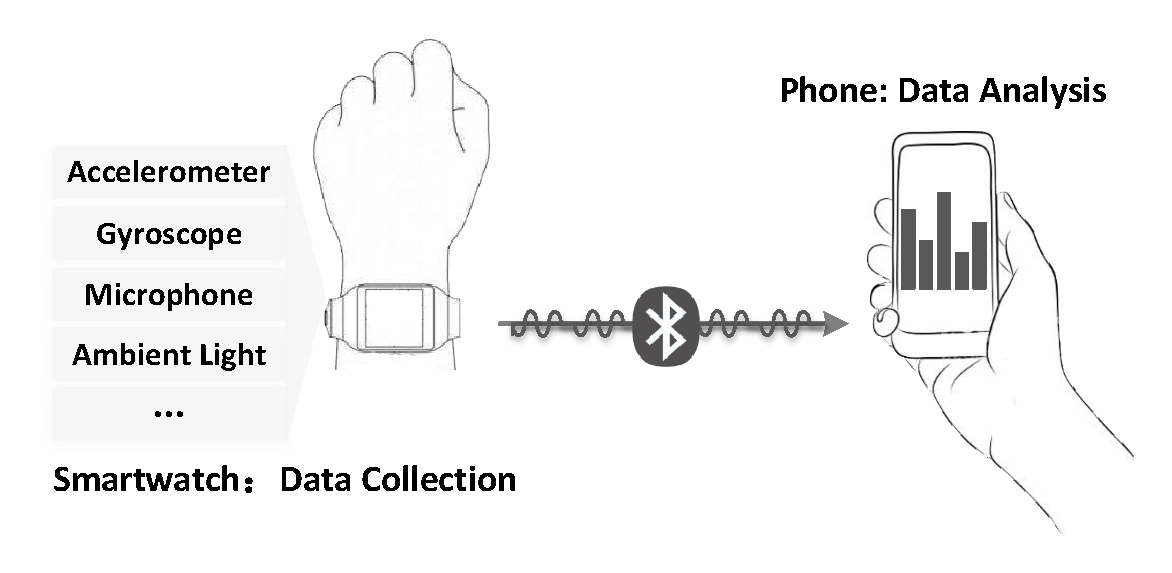
\includegraphics[width=0.5\textwidth]{Figures/datacollect.pdf}
%  \caption{Our approach detects a wide range of sleep-related activities and events using a smartwatch.}\label{fig:datacollect}
%\end{figure}

%advantages of using a smartwatch are that many users are willing to wear the device throughout the night, thus the device can remain
%relatively close to the user over the duration of sleep.



The present paper contributes by presenting the design and development of \systemname, a \emph{holistic sleep monitoring solution} that captures rich information about sleep events, the sleep environment, and the overall quality of sleep. \systemname is the first to solely rely on sensor information available on off-the-shelf smartwatches for capturing a wide range of sleep-related activities (see Table~\ref{tab:test}). The key insight in {\systemname} is that sleep quality is strongly correlated with characteristics of body movements, health related factors that can be identified from audio information, and characteristics of the sleep environment~\cite{shelgikar2016sleep}. By using a smartwatch, the sensors are close to the user during all stages of the night, enabling detailed capture of not only sleep cycles, but body movements and environmental changes taking place during the sleep period. Capturing these sleeping events from sensor data, however, is non-trivial due to changes in sensor measurements caused by hand motions during sleep. To overcome this challenge, changes in sensor orientation relative to user's body need to be tracked and opportune moments where to capture sensor data need to be detected. To address these issues, \systemname integrates a set of new methods for analysing and capturing sleep-related information from sensor measurements available on a smartwatch. \systemname also incorporates a model that uses the detected events to infer the user's sleep stages and sleep quality. While some prior research has examined the use of smartwatches for sleep monitoring~\cite{pombo2016ubisleep,shelgikar2016sleep,haescher2015anomaly,borazio2012combining}, these approaches have only been able to gather coarse-grained information about sleep and often required additional highly-specialized devices, such as pressure mattresses or image acquisition equipment to supplement the measurements available from the smartwatch. In this paper, we demonstrate that, for the first time, using {\em only a smartwatch}, it is possible to capture an extensive set of sleep-related information -- many of which are not presented in prior work. Having a more comprehensive set of sleep-related events and activities available enables users to gain a deeper understanding of their sleep patterns and the causes of poor sleep, and to make recommendations on how to improve one's sleep quality.



%We implement our approach in a prototype system called \systemname. It gathers sleep-related activities by utilizing the commonly available
%sensors on smartwatches: the accelerometer, gyroscope, microphone and ambient light sensor, etc. It then uses the tracked information to
%infer the user's sleep posture and habits -- thing like changes of body and hand positions, as well as sound events due to e.g. snoring or
%coughing.  Collecting these data can help a user to gain a deep understanding of his/her sleeping pattern and quality, and to find ways to
%improve sleep. \FIXME{ZW: The introduction is too wordy. It needs to get to the point quicker. I will get back to this later.}

  % \FIXME{ZW: This one needs to be merged with the previous paragraph.}

We evaluate \systemname through rigorous and extensive benchmark experiments conducted on data collected from fifteen participants during a
two week monitoring period. The results of our experiments demonstrate that \systemname can accurately characterize body motions and
movements during sleep, as well as capture different acoustic events. Specifically, the lowest accuracy for \systemname in our experiments
is 87\%, with the best event detection accuracy reaching up to 98\%. We also demonstrate
that \systemname can accurately detect various sleep stages and help users to better understand their sleep quality. During our experiments, six of the $15$ participants suffered from sleep quality problems, all of whom were correctly identified by \systemname. Moreover, we also demonstrate that \systemname is able to correctly identify the root cause of their sleep problems whether it is due to suboptimal hand position, body posture or sleeping environment. While the main objective of \systemname is not to estimate overall sleep quality, but to identify potential factors that disrupt sleep, we also demonstrate that \systemname provides sleep quality estimation that closely matches with subjective assessments and is comparable to Fitbit, a commercial state-of-the-art solution. Compared to Fitbit, the main advantage of \systemname is that can report a wider range of sleep events and provide a better understanding for the causes of sleep problems. %We show that \systemname successfully helps some of our testing users in
%finding the cause of poor sleep, 


\subsection*{Contributions}
This paper makes the following contributions:

\begin{itemize}[noitemsep]
	\item We present the design and development of \systemname (Section ~\ref{Sec:3design}), the first holistic sleep monitoring system to rely solely on sensors
available in an off-the-shelf smartwatch to capture a wide range of sleep information that characterizes overall sleep quality, user
behaviours during sleep, and the sleep environment.
	
\item We develop novel and lightweight algorithms for capturing sleep-related information on smartwatches taking into consideration
    changes in orientation and location of the device during different parts of the night. We show how to overcome specific challenges to
    effectively track events like sleep postures (Section~\ref{sec:sleeppdet}), hand positions (Section~\ref{sec:handpr}), body
    rollovers(Section~\ref{sec:bodyrollover}), micro body movement(Section~\ref{sec:microbo}), and acoustical
    (Section~\ref{sec:acoustic}) and lighting conditions (Section~\ref{sec:illumination}).


     %\textcolor{blue}{When we design these
%    algorithms, firstly, we found a key basis for sleeping posture detection that arms have common and (reasonably) stable positions in
%    each posture. Thus, we can build a mapping between the user's arms position and sleeping postures and identify the user's posture by
%    identifying periods where the hand is in a position that correlates with a specific posture. Secondly, we try to detect the position
%    of the hand based on another intuition��that is any change in hand position results in a movement trajectory that is uniquely
%    determined by the start and end position of the hand. However, we find that in practical applications, it is difficult for us to
%    obtain the starting position of the hand every time, so rely on the trajectory of the hand movement does not work. In the end, we
%    based on a key intuition is that respiratory lead to the movement of the abdomen and chest, making the acceleration signals to
%    exhibit a distinctly periodic fluctuation. We can use the occurrence of respiratory events to determine if the hand is indeed on the
%    body (abdomen or chest). Thirdly, when we detect the body rollover events, we avoided using the methods of detecting the direction of
%    rotation of the arm or the tilt of the wrist during movement of the body. Although these two methods seem to be effective, but in the
%    actual sleep process, the error they get is very large. To deal with this challenge, we incorporate the body postures to improve the
%    detection accuracy. It is based on the simple fact that the body postures are different before and after the rollover. Nextly, we
%    detect the micro body movement based on the signal duration time and the first-order derivative of the acceleration, in order to
%    realize the classification of more micro motions. In addition, we also designed two interesting algorithms, namely the detection of
%    acoustic events, changing the traditional complex algorithm multi-dimensional signal feature extraction, instead, it is through
%    mining the essential characteristics of events, that is exploiting the inherent characteristics of different acoustic event to
%    detect. And the other algorithm is illumination conditions detection, we use the movement of the hand to avoid the problem of
%    unstable reading of the light sensor.}
	

    \item We extensively evaluate the performance of \systemname using measurements collected from two-week monitoring of $15$
        participants (Section~\ref{sec:expsetup}). Our results demonstrate that \systemname can accurately capture a wide range of sleep events,
        estimate different sleep stages, and produce meaningful information about overall sleep quality (Section~\ref{sec:4experiment}).  We show
        that \systemname successfully reveals the causes of poor sleeps for some of our testing users and subsequently helps them improve
        their sleep by changing their sleep behaviours and sleeping environment (Section~\ref{sec:user_survey}).
\end{itemize}

%To summarize, the main contribution of this paper is the first smartwatch-based system that can capture a wider range of sleep events with a high
%accuracy. We show that, compared with existing mobile-based sleep monitoring solutions, the rich set of fine-grained sleep events given by
%o%
%ur approach can better capture a user's sleep patterns and quality across sleep stages.

%ZW: I have commented out the motivation section as it reads like related work.
%\input{motivation.tex}
%%\subsection{Overview of \systemname}

%\begin{figure}
%  \centering
  % Requires \usepackage{graphicx}
 % 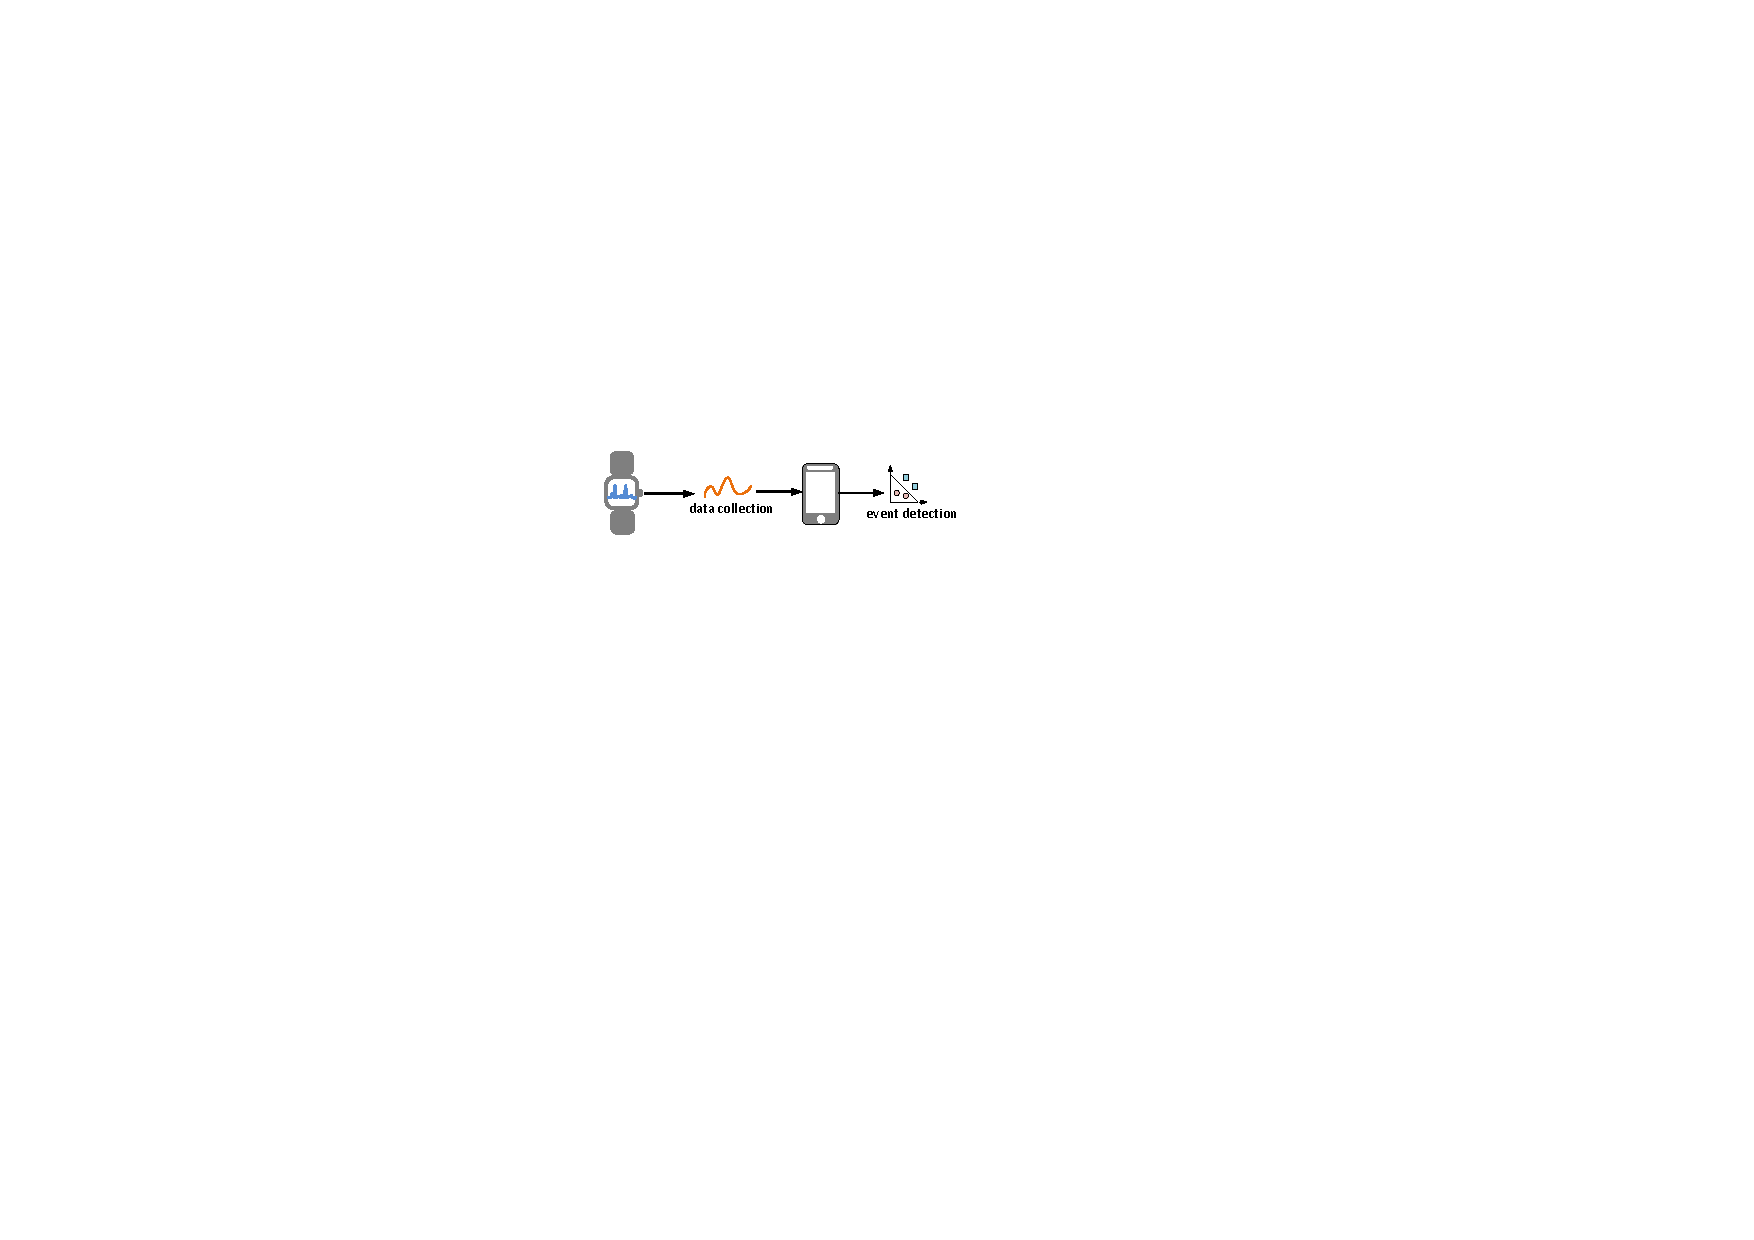
\includegraphics[width=0.7\textwidth]{figures/overviewd.pdf}\\
 %\caption{Overview of our 2-stage approach. Sleep data are collected through smartwatch sensors, which are then passed to be processedby a mobile app
%  to detect sleep events.}\label{fig:overview}
%\end{figure}

\systemname is a novel smartwatch-based sleep monitoring system that aims at estimating sleep quality and capturing rich information about
behaviours and events occurring during sleep. By capturing this information, \systemname can analyze potential reasons for sleep problems
and provide the user with suggestions on how to improve their sleep routine or sleep environment. To achieve its design goal, \systemname
exploits a wide range of sensors that are common on commercial off-the-shelf smarwatches: (i) accelerometer, gyroscope, and orientation
sensor are used to collect body and hand movements; (ii) microphone is used to measure level of ambient noise and to capture acoustic
events; and (iii) ambient light sensor is used to monitor illumination within the sleep environment. The different sensors and information
extracted from them are summarized in Table~\ref{tab:test}. In the following we discuss the different subcomponents of \systemname in
detail.

%acoustic data, the ambient light sensor for illumination conditions, the orientation sensor for calibration. The collected data are
%transmitted to a smartphone via Bluetooth. We propose a set of new analysis and algorithms to effectively detect sleep events from the
%collected data. Table~\ref{tab:test} lists the set of sleep events supported by \systemname.
%Figure~\ref{fig:overview} depicts our 2-stage approach that involves collecting data using a smartwatch and sleep event detection using a
%smartphone. Sleep data are collected using smartwatches sensors. Our work

\begin{table}[t!]
 \caption{\label{tab:test}Sleep events targeted in this work}
 \centering
 \begin{tabular}{ll}
  %\toprule
  \toprule
  \textbf{Event}& \textbf{Type} \\
  \midrule
\rowcolor{Gray}  Sleep postures & Supine, Left lateral, Left lateral, Prone\\
 Hand positions & Head, Chest, Abdomen\\
\rowcolor{Gray} Body rollover & Count\\
 Micro body movements& Hand moving, Arm raising, Body trembling \\
\rowcolor{Gray} Acoustic events & Snore, Cough, Somniloquy  \\
 Illumination condition & Strong, Weak  \\
  \bottomrule
 %\hline
 \end{tabular}
\end{table}

%\begin{figure}[!thbp]
%\centering
%%\setlength{\belowcaptionskip}{-9pt}
%      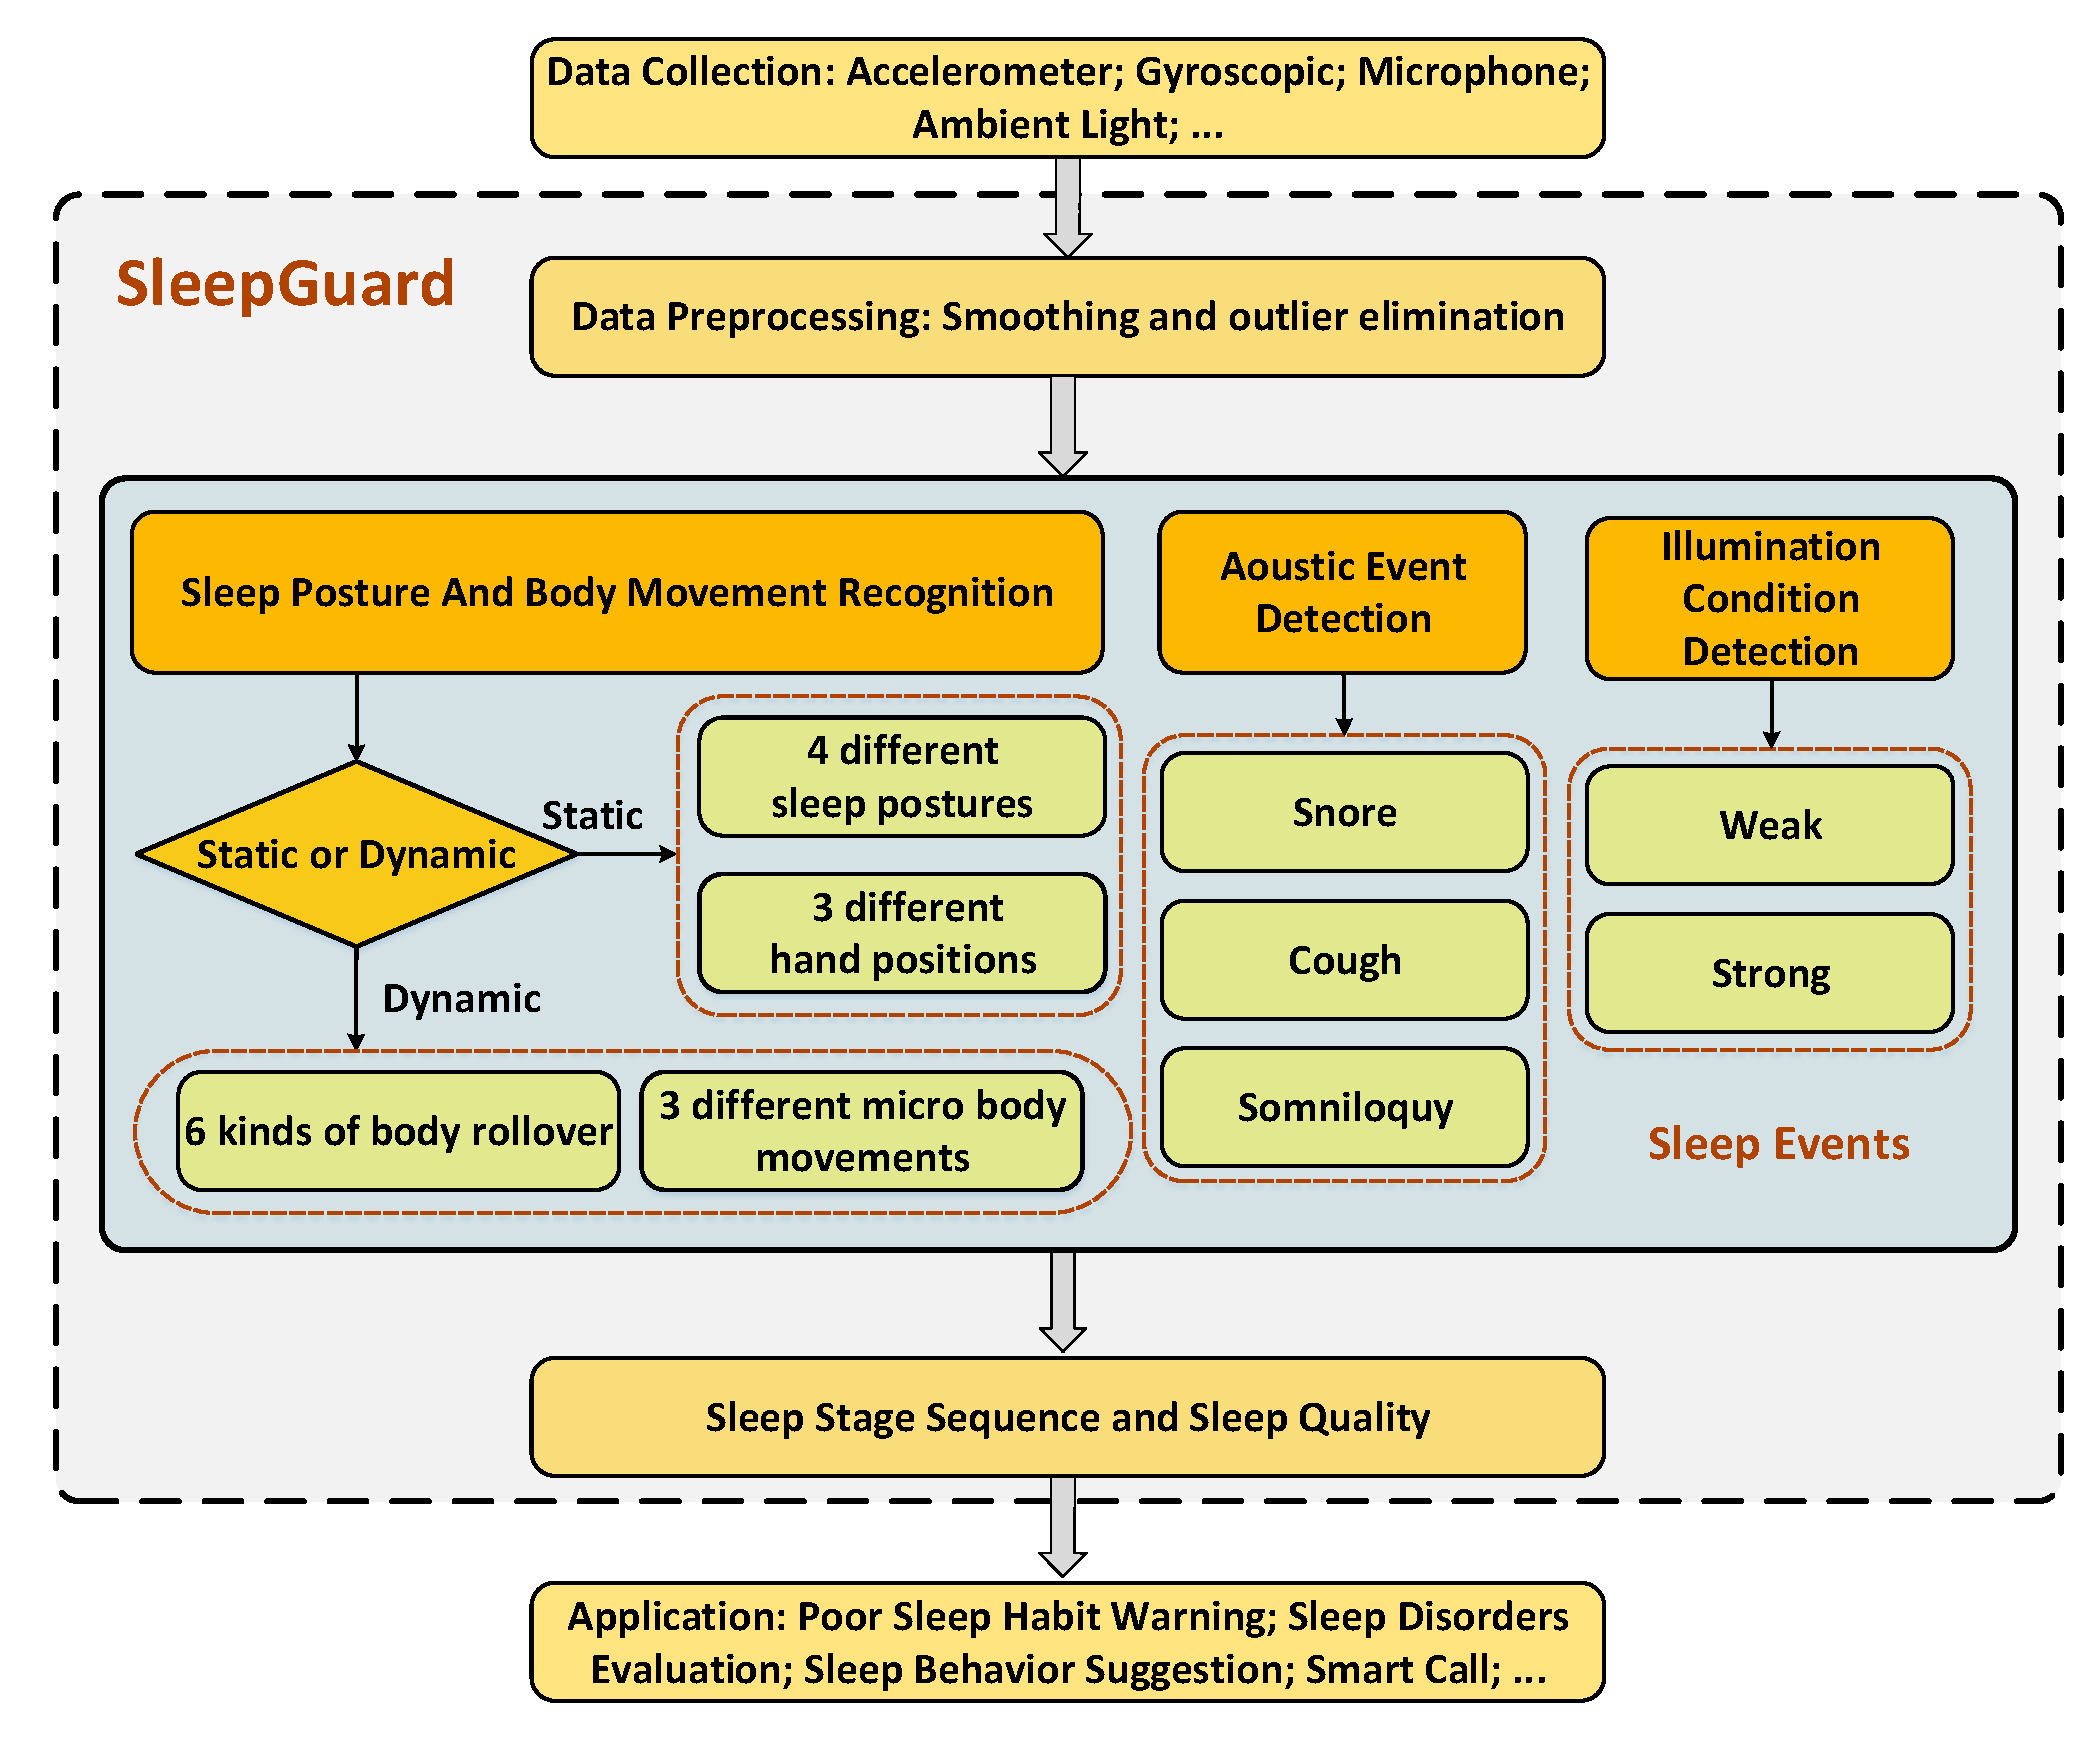
\includegraphics[width=0.97\linewidth]{Figures/SystemFlow.pdf}
%  \caption{System overview of {\systemname}.}\label{fig:overview}
%\end{figure}
%
%
%\begin{itemize}[itemsep=1mm,nolistsep]
%  \item {\textbf{Data Collection and Preprocessing.}} A variety of sensing data are related to sleep events include i) the accelerometer and the gyroscope about the body movement, ii) the microphone measured acoustic sound, iii) the ambient light sensor about the illumination condition, and iv) the orientation sensor with some auxiliary information. The data is collected every 30 ms on the smartwatch and transferred to the server (such as a smartphone) via Bluetooth. We use data smoothing and outlier elimination to reduce noise in the raw sensor readings.
%  \item \textbf{Sleep Event Detection.} A series of novel algorithms are developed to recognize different sleep events. In particular, some key insights are observed about different body postures, body rollovers, hand positions, micro body movements and acoustic events. Note that before identifying those events, {\systemname} first carries out a coarse-grained detection and judges whether the user is lying or not.  After that, we can estimate the user's bedtime. During the user is lying on the bed,  we regard that the user fell asleep if we do not detect a large movement within 20 minutes.
%  \item \textbf{{Sleep Pattern Report.}} Sleep Pattern Report. After we obtain the detected sleep events, we integrate them to the clock information, illumination condition, and then use the Hidden Markov Model to infer the sleep stages and evaluate sleep quality. Different from existing apps on the market, {\systemname} provides detailed procedure about the sleep report. The output of our system, for example, sleep postures and the position of user's hand could be used as input to build a broad range of sleeping quality and  heathy applications, such as poor sleep habit warning, the evaluation of insomnia, nightmare and sleep disorders. With the extensive experiments conducted, we conclude that {\systemname} exhibits a relatively high accuracy comparing to state-of-the-art systems.
%\end{itemize}


%\subsection{Feature Calculation and Selection}
%Appropriate  features  can  reflect  the  potential  information  underlying the  signals. The  features  used  in {\systemname} are shown in  Table \ref{Tab1}. To detect different sleep events, we use two main features. The first one is the movement related features, that are angle of inclination calculated by acceleration data and the angle of rotation calculated by gyroscopic data. Beyond that, to detect different sound events during sleep, we calculate the energy and zero-crossing rate of the sound signal.
%
%\begin{table}[!thbp]
%\centering
% \caption{Calculated Features}\label{Tab1}
%   \renewcommand\arraystretch{1.7}{\multirowsetup}{\centering}
%        \begin{tabular}{c|c|c}
%        \hline
%        {\bf{Data}}  &   {\bf{Feature}} &   {\bf{Formula}}\\
%         \hline
%        {$acc$} & {Tilt Angle}   & $ A_x =\arccos(\frac {acc_x}{acc}) $ \\
%        \hline
%        {$\omega$} &  {Rotation Angle}  & $ \theta = \int\omega $ \\
%        \hline
%        %\multirow{2} {0.1cm}
%        {Sound}  & Energy   &$ E=\sum\nolimits_{n=-\infty}^{\infty}|x^2(n)|$ \\
%         {$x(n)$}  & Zero-crossing  & $Z$ \\
%          \hline
%\end{tabular}
%\end{table}

\section{\systemname Sleep Monitoring Platform}\label{Sec:3design}

%\subsection{Overview of \systemname}

%\begin{figure}
%  \centering
  % Requires \usepackage{graphicx}
 % 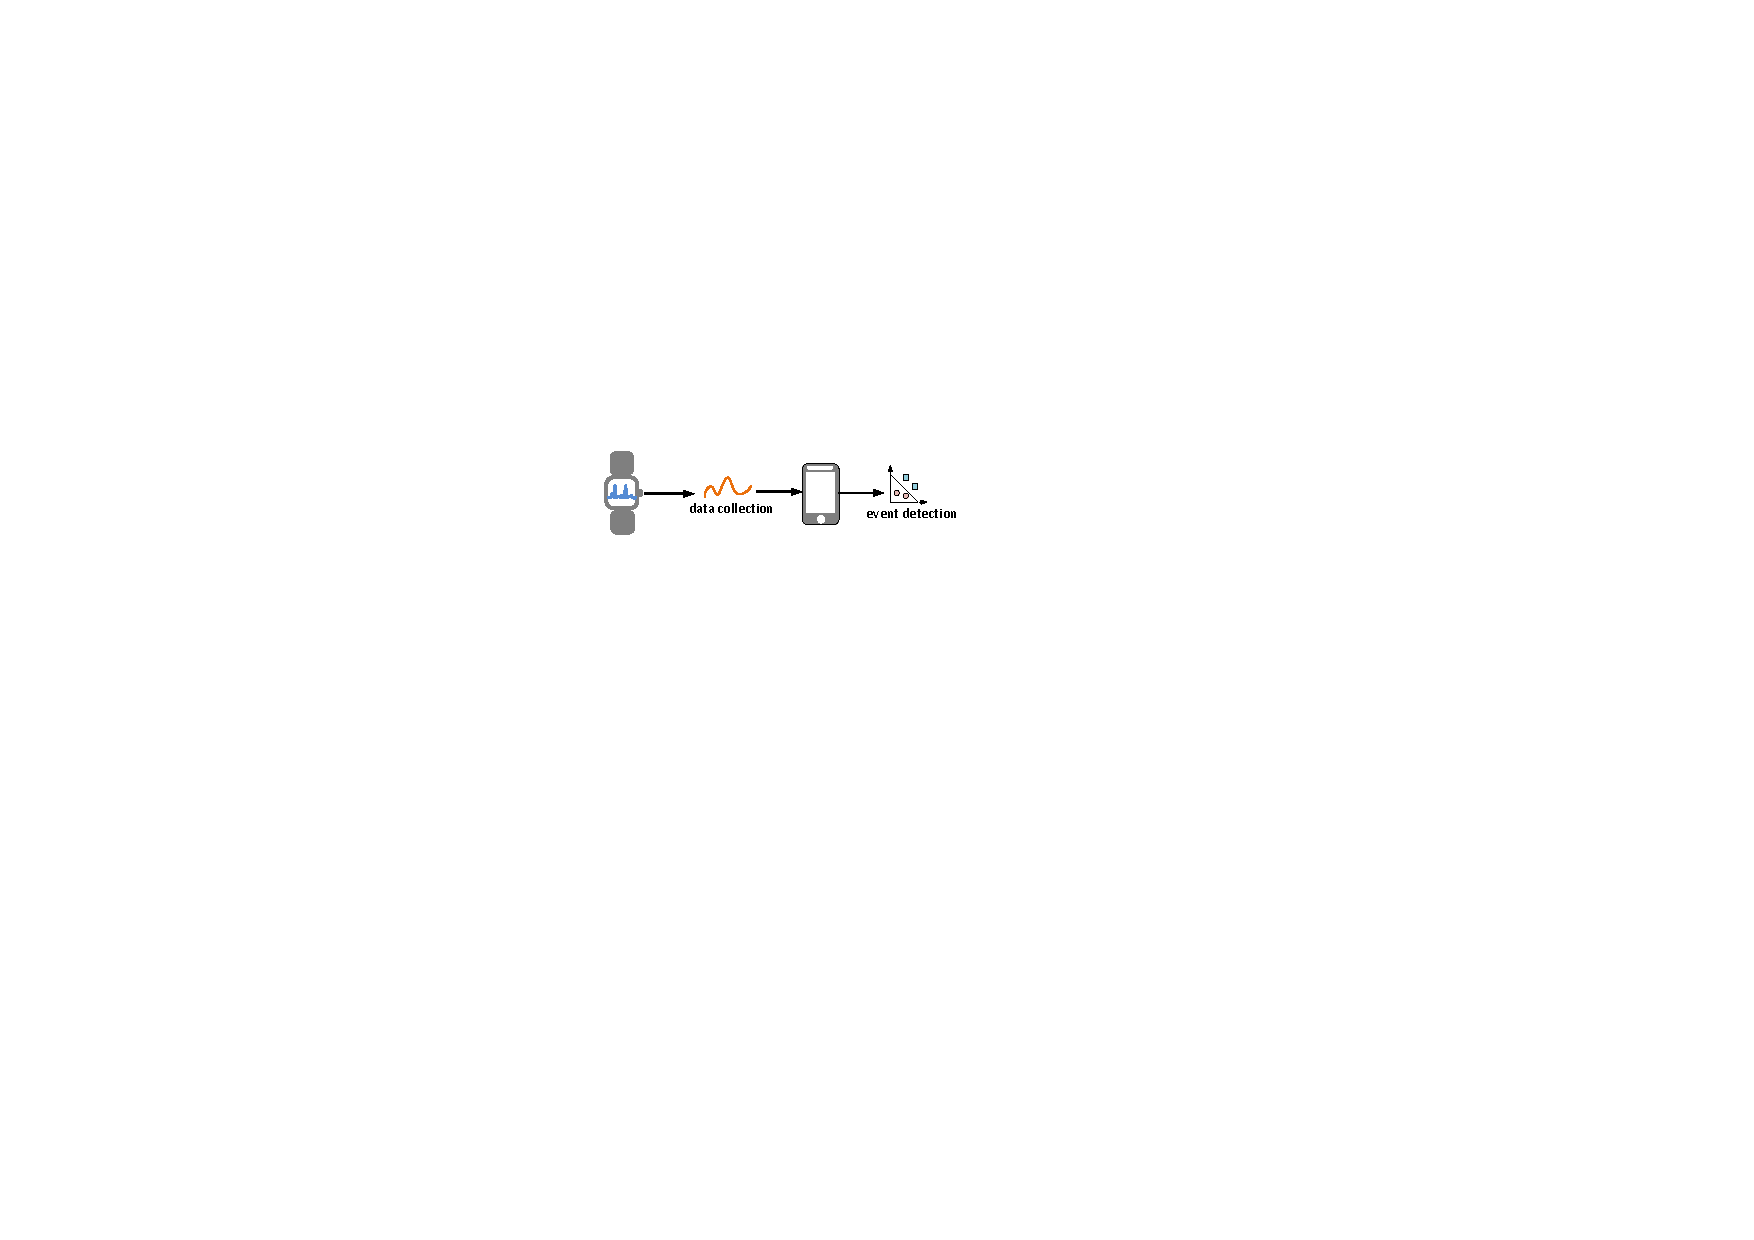
\includegraphics[width=0.7\textwidth]{figures/overviewd.pdf}\\
 %\caption{Overview of our 2-stage approach. Sleep data are collected through smartwatch sensors, which are then passed to be processedby a mobile app
%  to detect sleep events.}\label{fig:overview}
%\end{figure}

\systemname is a novel smartwatch-based sleep monitoring system that aims at estimating sleep quality and capturing rich information about
behaviours and events occurring during sleep. By capturing this information, \systemname can analyze potential reasons for sleep problems
and provide the user with suggestions on how to improve their sleep routine or sleep environment. To achieve its design goal, \systemname
exploits a wide range of sensors that are common on commercial off-the-shelf smarwatches: (i) accelerometer, gyroscope, and orientation
sensor are used to collect body and hand movements; (ii) microphone is used to measure level of ambient noise and to capture acoustic
events; and (iii) ambient light sensor is used to monitor illumination within the sleep environment. The different sensors and information
extracted from them are summarized in Table~\ref{tab:test}. In the following we discuss the different subcomponents of \systemname in
detail.

%acoustic data, the ambient light sensor for illumination conditions, the orientation sensor for calibration. The collected data are
%transmitted to a smartphone via Bluetooth. We propose a set of new analysis and algorithms to effectively detect sleep events from the
%collected data. Table~\ref{tab:test} lists the set of sleep events supported by \systemname.
%Figure~\ref{fig:overview} depicts our 2-stage approach that involves collecting data using a smartwatch and sleep event detection using a
%smartphone. Sleep data are collected using smartwatches sensors. Our work

\begin{table}[t!]
 \caption{\label{tab:test}Sleep events targeted in this work}
 \centering
 \begin{tabular}{ll}
  %\toprule
  \toprule
  \textbf{Event}& \textbf{Type} \\
  \midrule
\rowcolor{Gray}  Sleep postures & Supine, Left lateral, Left lateral, Prone\\
 Hand positions & Head, Chest, Abdomen\\
\rowcolor{Gray} Body rollover & Count\\
 Micro body movements& Hand moving, Arm raising, Body trembling \\
\rowcolor{Gray} Acoustic events & Snore, Cough, Somniloquy  \\
 Illumination condition & Strong, Weak  \\
  \bottomrule
 %\hline
 \end{tabular}
\end{table}

%\begin{figure}[!thbp]
%\centering
%%\setlength{\belowcaptionskip}{-9pt}
%      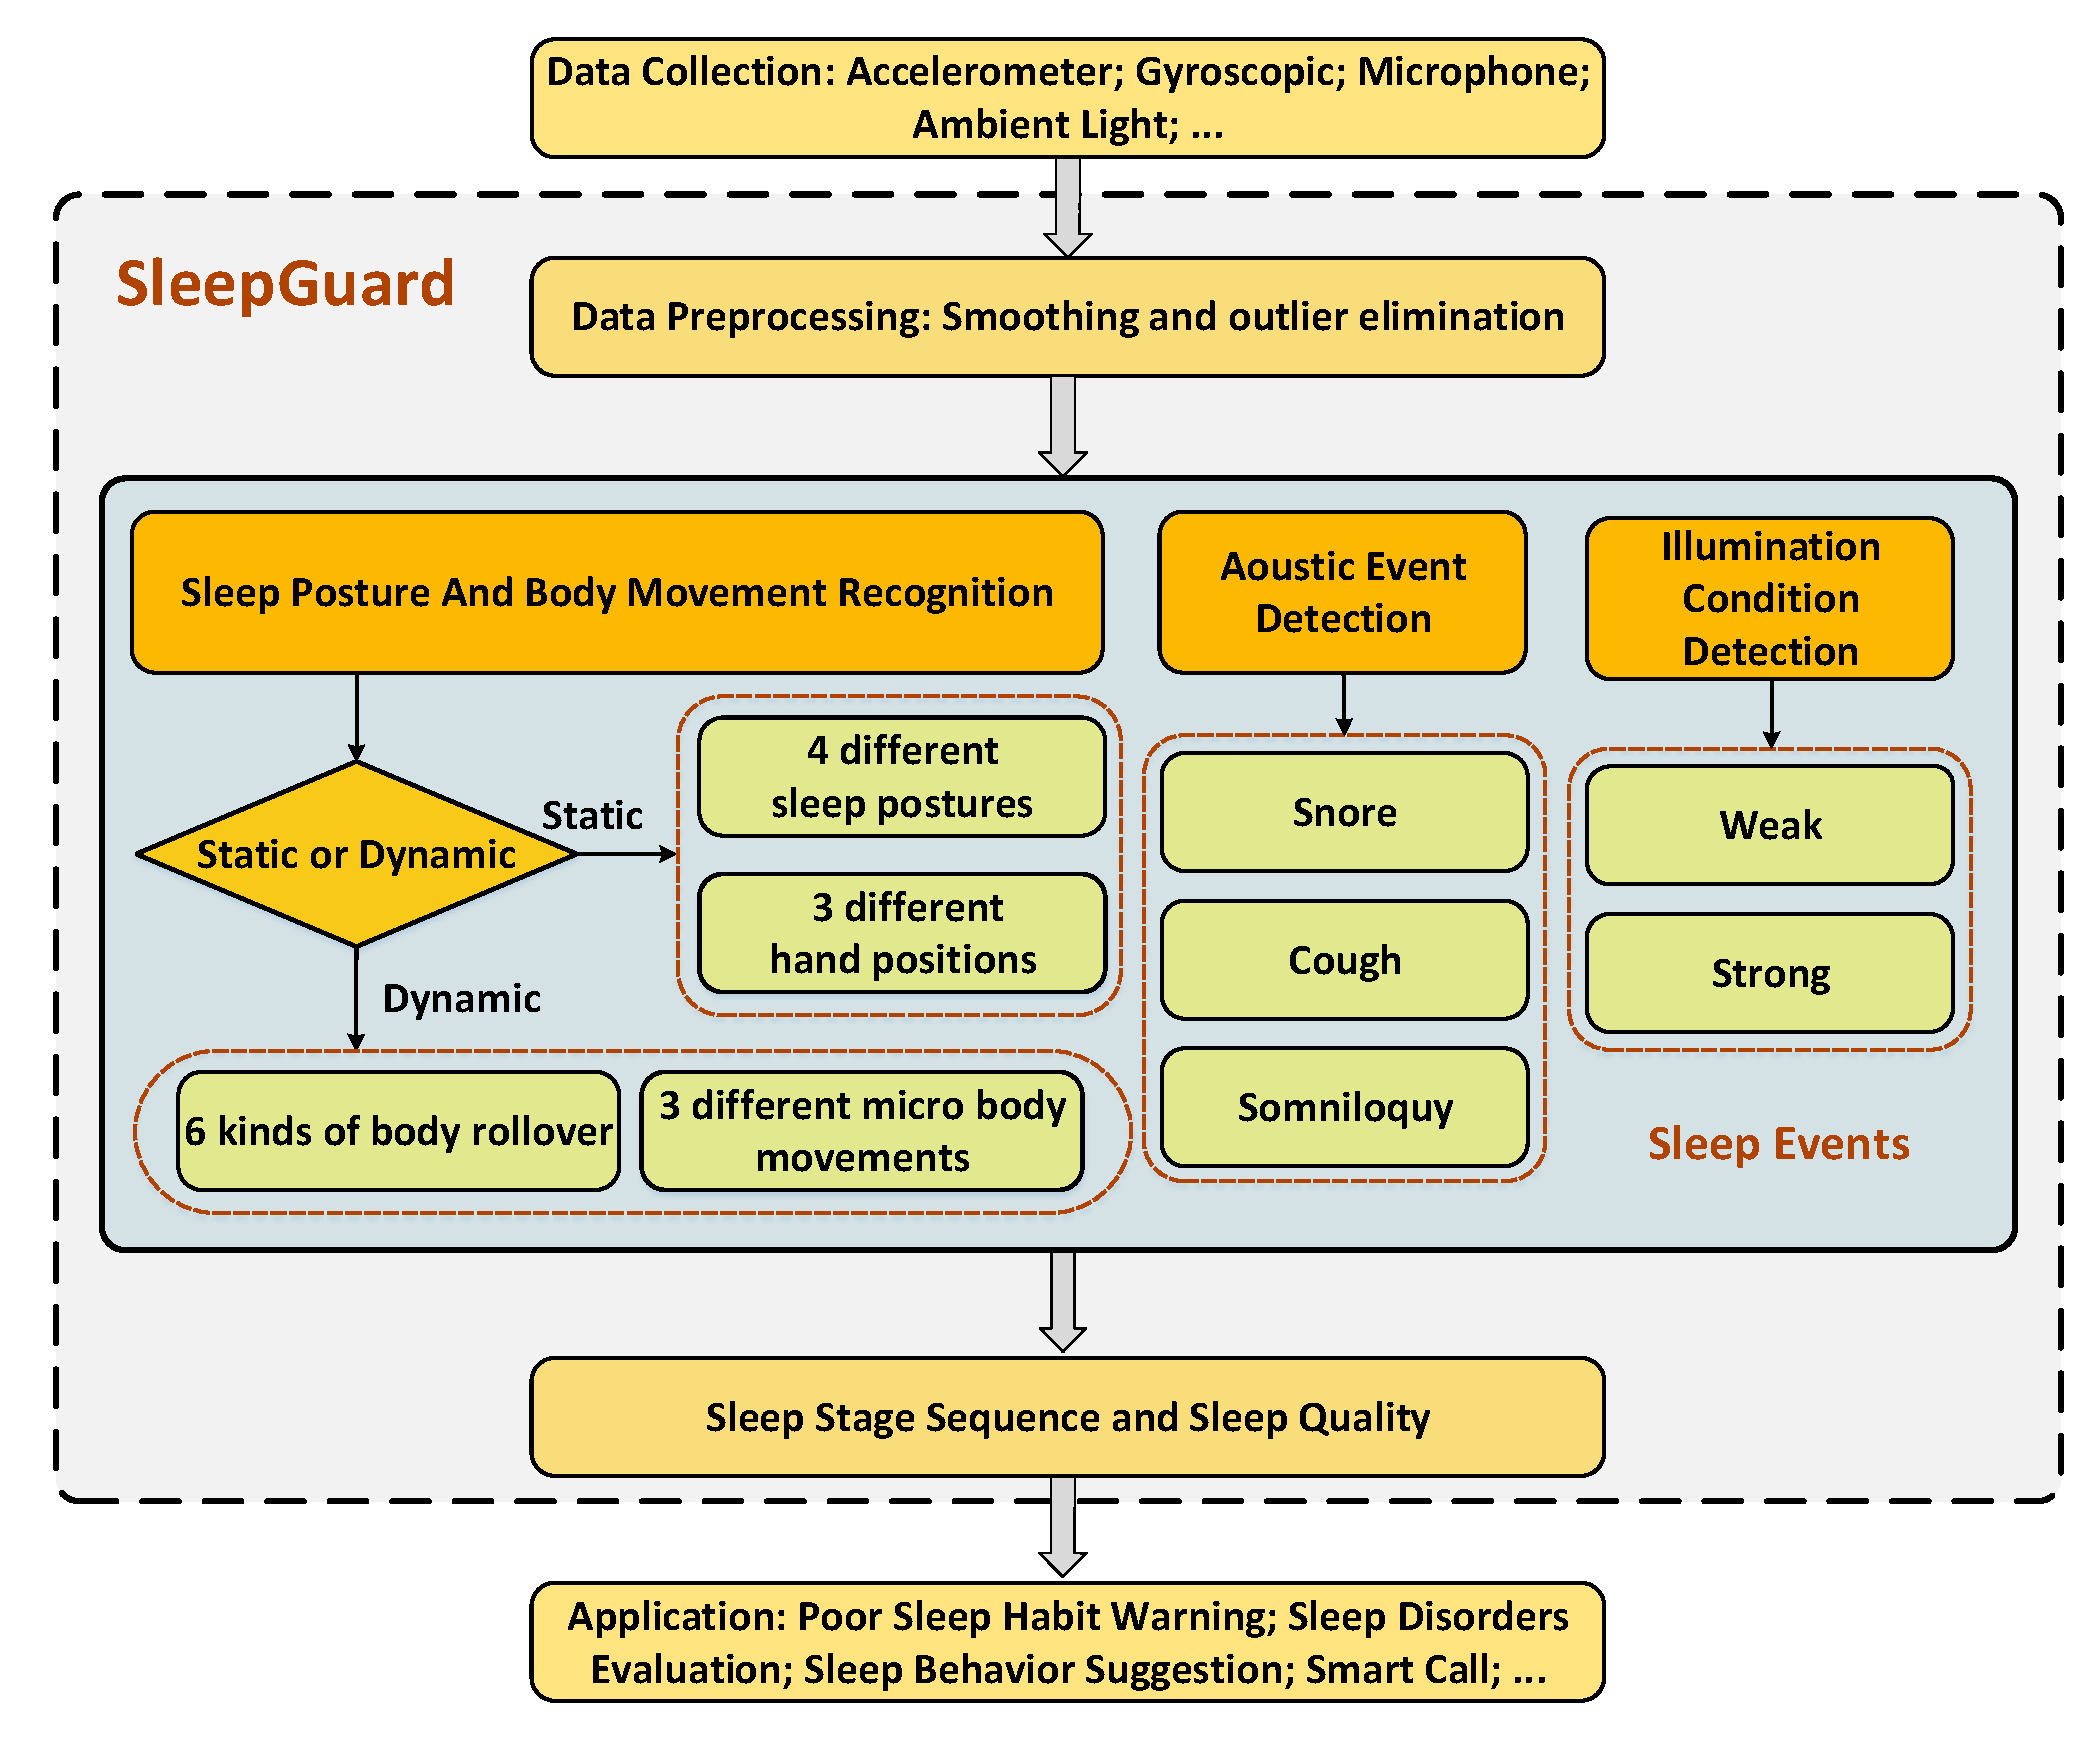
\includegraphics[width=0.97\linewidth]{Figures/SystemFlow.pdf}
%  \caption{System overview of {\systemname}.}\label{fig:overview}
%\end{figure}
%
%
%\begin{itemize}[itemsep=1mm,nolistsep]
%  \item {\textbf{Data Collection and Preprocessing.}} A variety of sensing data are related to sleep events include i) the accelerometer and the gyroscope about the body movement, ii) the microphone measured acoustic sound, iii) the ambient light sensor about the illumination condition, and iv) the orientation sensor with some auxiliary information. The data is collected every 30 ms on the smartwatch and transferred to the server (such as a smartphone) via Bluetooth. We use data smoothing and outlier elimination to reduce noise in the raw sensor readings.
%  \item \textbf{Sleep Event Detection.} A series of novel algorithms are developed to recognize different sleep events. In particular, some key insights are observed about different body postures, body rollovers, hand positions, micro body movements and acoustic events. Note that before identifying those events, {\systemname} first carries out a coarse-grained detection and judges whether the user is lying or not.  After that, we can estimate the user's bedtime. During the user is lying on the bed,  we regard that the user fell asleep if we do not detect a large movement within 20 minutes.
%  \item \textbf{{Sleep Pattern Report.}} Sleep Pattern Report. After we obtain the detected sleep events, we integrate them to the clock information, illumination condition, and then use the Hidden Markov Model to infer the sleep stages and evaluate sleep quality. Different from existing apps on the market, {\systemname} provides detailed procedure about the sleep report. The output of our system, for example, sleep postures and the position of user's hand could be used as input to build a broad range of sleeping quality and  heathy applications, such as poor sleep habit warning, the evaluation of insomnia, nightmare and sleep disorders. With the extensive experiments conducted, we conclude that {\systemname} exhibits a relatively high accuracy comparing to state-of-the-art systems.
%\end{itemize}


%\subsection{Feature Calculation and Selection}
%Appropriate  features  can  reflect  the  potential  information  underlying the  signals. The  features  used  in {\systemname} are shown in  Table \ref{Tab1}. To detect different sleep events, we use two main features. The first one is the movement related features, that are angle of inclination calculated by acceleration data and the angle of rotation calculated by gyroscopic data. Beyond that, to detect different sound events during sleep, we calculate the energy and zero-crossing rate of the sound signal.
%
%\begin{table}[!thbp]
%\centering
% \caption{Calculated Features}\label{Tab1}
%   \renewcommand\arraystretch{1.7}{\multirowsetup}{\centering}
%        \begin{tabular}{c|c|c}
%        \hline
%        {\bf{Data}}  &   {\bf{Feature}} &   {\bf{Formula}}\\
%         \hline
%        {$acc$} & {Tilt Angle}   & $ A_x =\arccos(\frac {acc_x}{acc}) $ \\
%        \hline
%        {$\omega$} &  {Rotation Angle}  & $ \theta = \int\omega $ \\
%        \hline
%        %\multirow{2} {0.1cm}
%        {Sound}  & Energy   &$ E=\sum\nolimits_{n=-\infty}^{\infty}|x^2(n)|$ \\
%         {$x(n)$}  & Zero-crossing  & $Z$ \\
%          \hline
%\end{tabular}
%\end{table}




\begin{figure*}
	\centering
	\begin{minipage}[t]{.33\textwidth}
		\centering
		  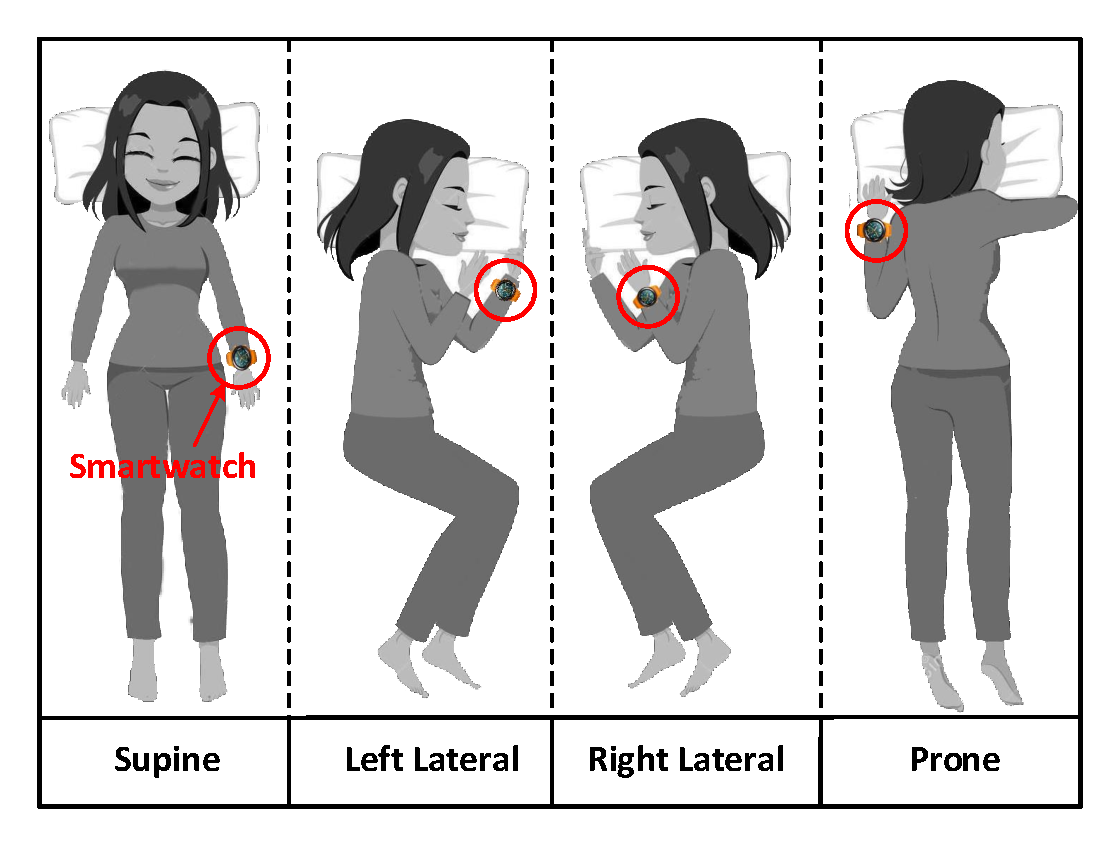
\includegraphics[width=4.7cm,height=3.7cm]{Figures/BodyPosture.pdf}
		\caption{Four sleep body postures.}
		\label{fig:BodyPosture}
	\end{minipage}%
	\begin{minipage}[t]{.33\textwidth}
		\centering
		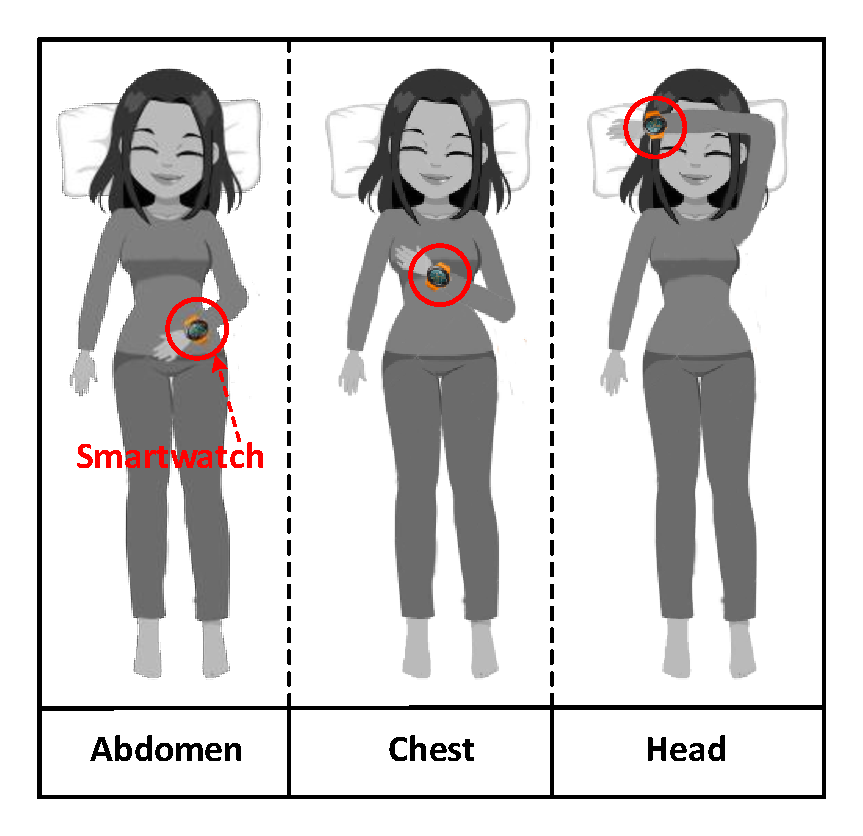
\includegraphics[width=4.1cm,height=3.4cm]{Figures/HandPosition.pdf}
		\caption{Three hand positions.}
		\label{fig:HandPosition}		
	\end{minipage}
\begin{minipage}[t]{.33\textwidth}
		\centering
	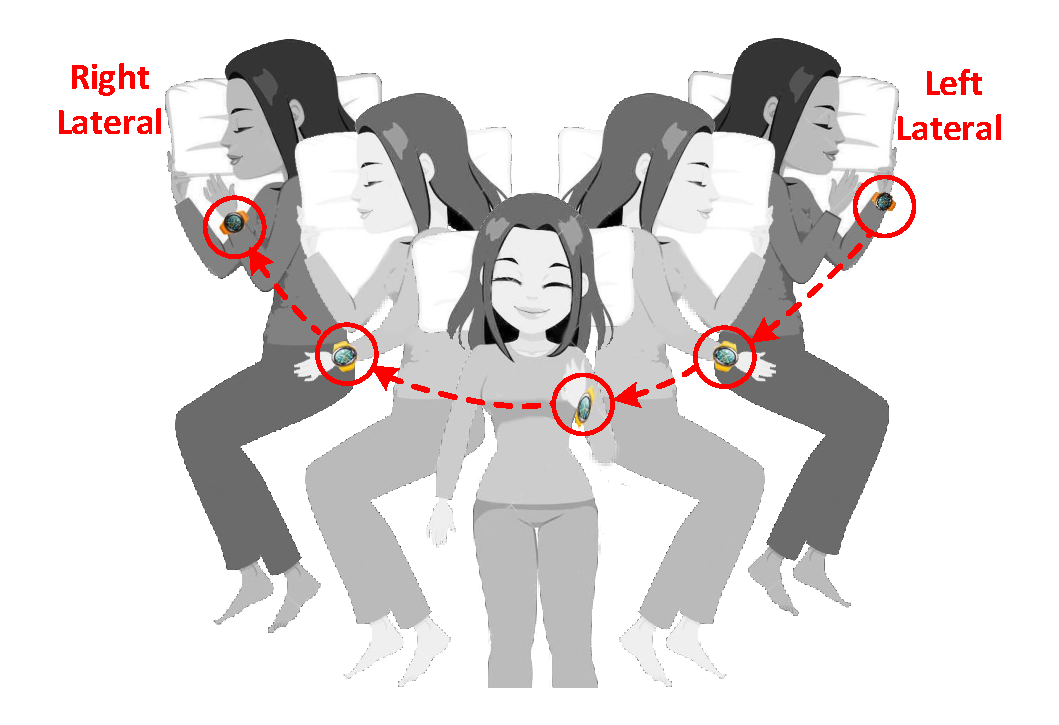
\includegraphics[width=4.7cm,height=3.7cm]{Figures/BodyRollover.pdf}
	\caption{Body rollover from the left side to the right side.}
	\label{fig:BodyRollover}
\end{minipage}
\end{figure*}


\subsection{Detecting Sleep Postures and Movements}

One's sleeping position, also referred to as {\em sleep posture}, and the extent of body movements are important factors in determining overall sleep quality. Suboptimal posture has been shown to affect the severity of sleep disorders and is widely used in medical diagnoses to analyse effects of sleep disorders~\cite{oksenberg1998effect,eiseman2012impact} while having a good sleep posture has been shown to correlate with subjective assessments of sleep quality~\cite{dekoninck83sleep}. Similarly, high degree of body movements during sleep likely reflects restlessness, which results in poor sleep quality. {\systemname} uses motion sensors (accelerometer, gyroscope, and orientation sensor) to capture user's sleep posture and habits. In the following we detail the techniques we use for capturing the body posture and movements.  {\systemname}, currently supports the 4 basic sleep postures (see Fig.~\ref{fig:BodyPosture}); 3 hand positions (see Fig.~\ref{fig:HandPosition}); 6 types of body rollovers (see Fig.~\ref{fig:BodyRollover} for an example); and 3 types of body micro movements. %These events comprehensively and highly relate to the sleep stages and quality.


\subsubsection{Sleep Posture Detection\label{sec:sleeppdet}}

Dreaming and sleep quality are associated with underlying brain functions, which in turn are affected by body posture~\cite{posture2004}.
Sleep posture also varies across individuals and should fit personal and physical needs of the individual~\cite{posture2016,posture2017}.
For example, sleeping in a prone position is unsuitable for people with ailments, such as heart disease or high blood pressure. On the
other hand, people can consciously avoid postures that would be beneficial for health and sleep quality~\cite{posture2015}. Having an
effective way to detect the current posture and track changes in it would thus be essential for estimating overall sleep quality, and
avoiding potential harm. \systemname captures the four basic sleep postures, which are supine, left lateral, right lateral, and prone. This
is illustrated in Fig.~\ref{fig:BodyPosture}. However, detecting these postures using a single wrist sensor is non-trivial because the
sensor cannot accurately track the entire body movement. We observe that the arm position strongly correlates to the sleep postures, i.e.,
the arm is typically located in a specific, stable location for a given sleep posture. This observation suggests that we can first identify
the user's arm position and the duration of a specific arm location, and then map the information to a sleep posture. Later in this paper
(\FIXME{Section xx}), we show that our approach can achieve a high accuracy in identifying sleep postures.




%\textcolor{blue}{As we all know, it is very difficult to use only a smartwatch to describe
%the posture of the entire body, but we found a key basis for sleeping posture detection through observation and a pilot (see Sec. 3.1).}
%The key intuition for distinguishing between these postures is that arms have common and (reasonably) stable positions in each posture.
%\textcolor{blue}{Thus, we can build a mapping between the user's arms position and sleeping postures and identify the user's posture by
%identifying periods where the hand is in a position that correlates with a specific posture.} The basic idea is similar to the posture
%recognition used in~\cite{sleepmonitor}, but we use an additional step to improve the accuracy of distinguishing between supine and prone
%positions.

To separate sleep postures, {\systemname} considers a set of feasible hand positions for each posture. In the supine position, we assume the user's hand to be on the left side of the body, on the abdomen, on the chest or on the head; in the left and right lateral positions, we assume the user's hand is close to the pillow, on the chest or on the waist. Finally, in the prone position we assume the user's hand is on the side of the head or above his/her head. These positions were selected based on a pilot carried out in our test environment (see Sec.~\ref{sec:expsetup}). Fig.~\ref{fig:BodyPosture} shows one possible hand position for each of the postures.

\begin{figure}
	\centering
	\subfigure[Supine]{
		\label{fig:Supine}
		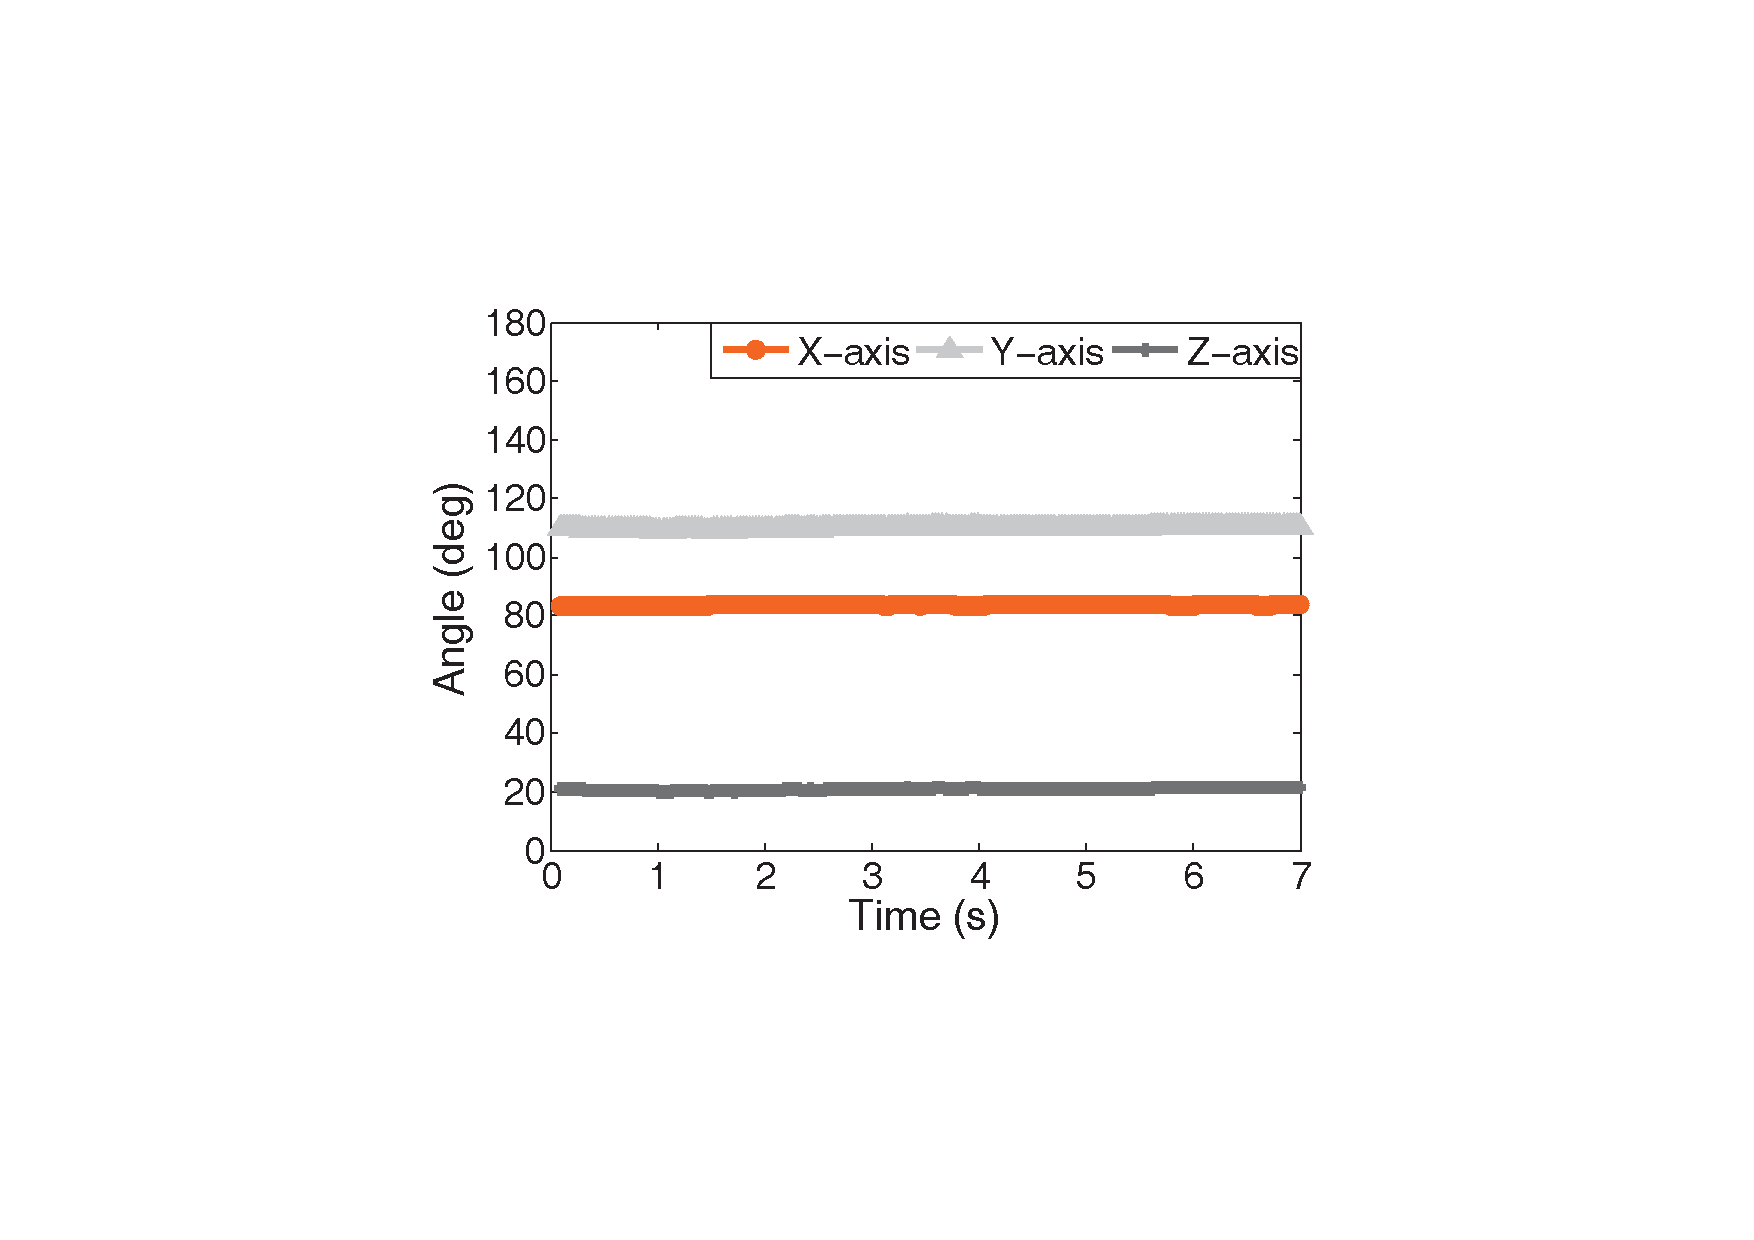
\includegraphics[width=0.24\linewidth]{Figures/Supine.pdf}}
	\hfill
	\subfigure[Left Lateral]{
		\label{fig:LeftLateral}
		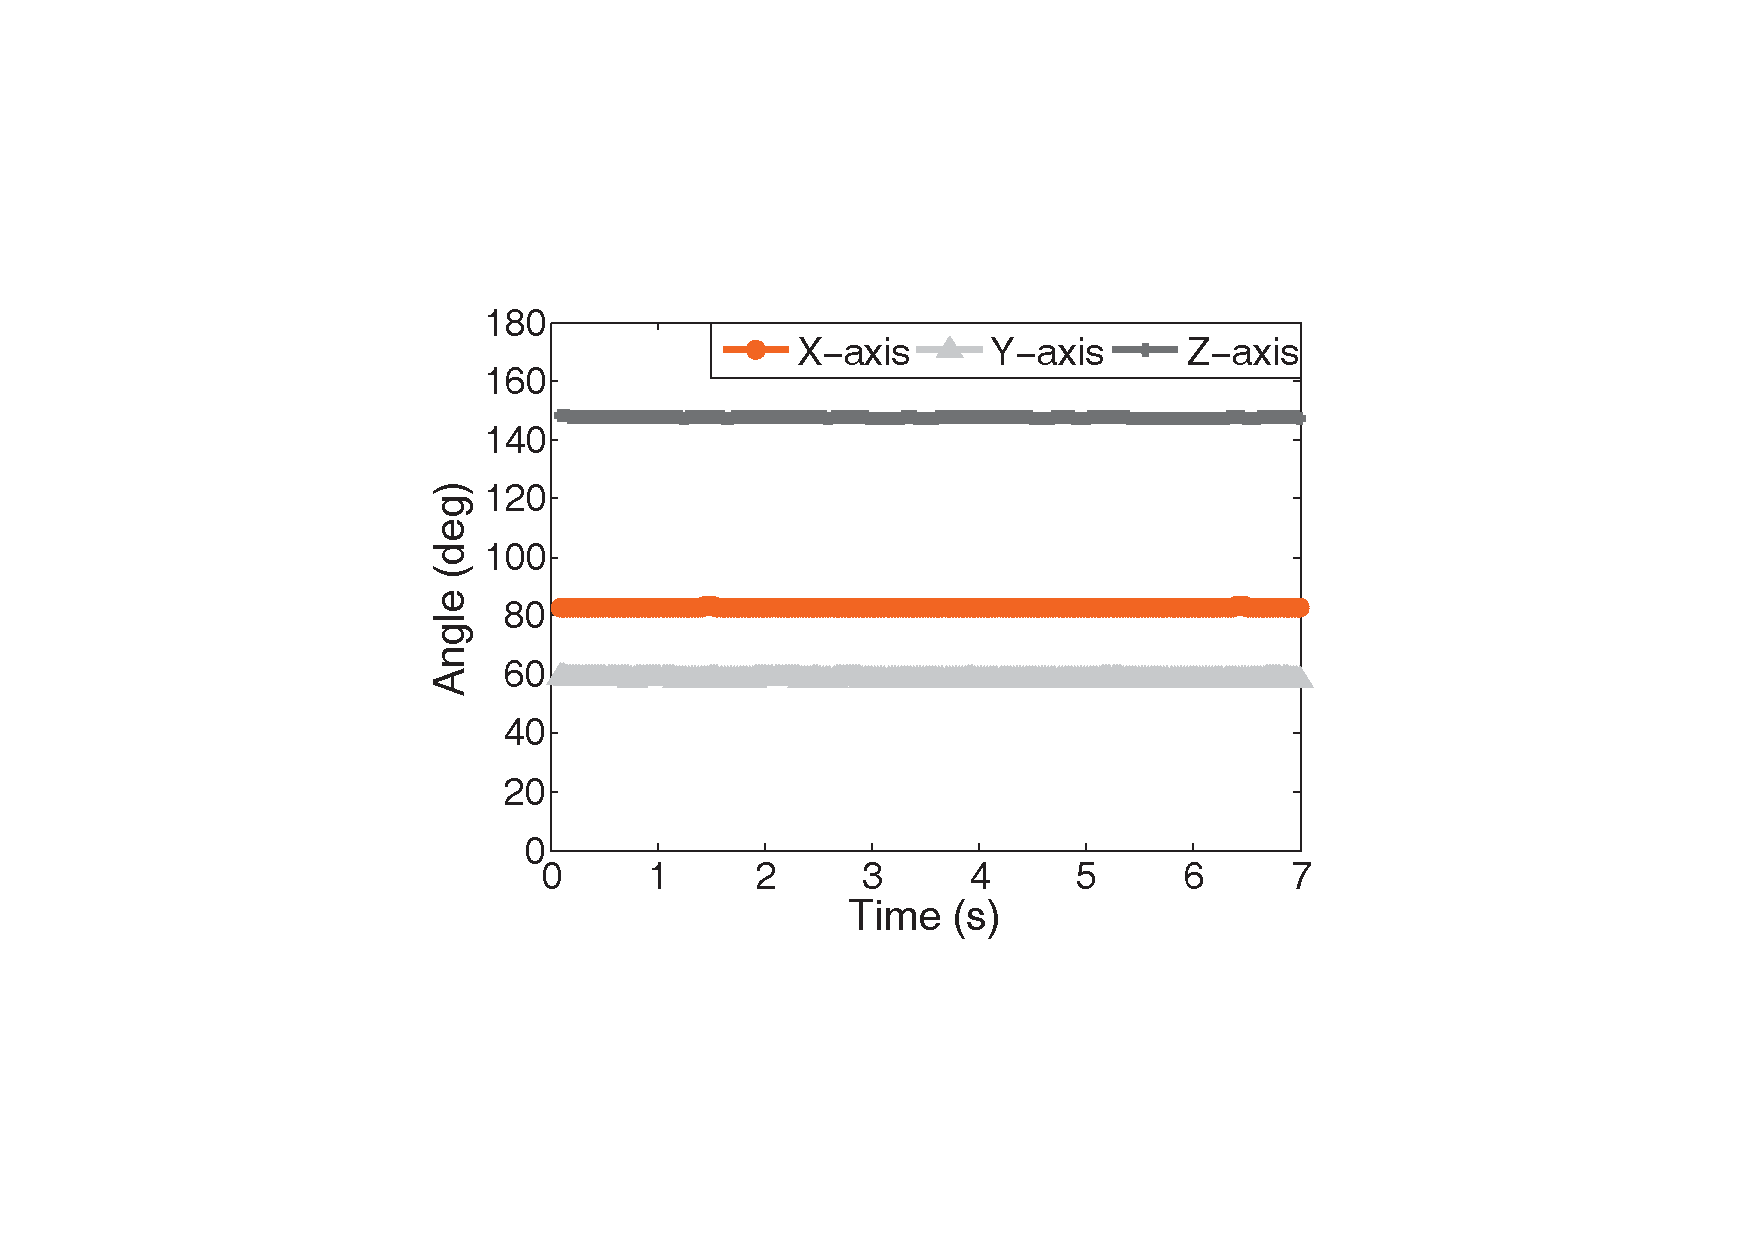
\includegraphics[width=0.24\linewidth]{Figures/LeftLateral.pdf}}
	\subfigure[Right Lateral]{
		\label{fig:RightLateral}
		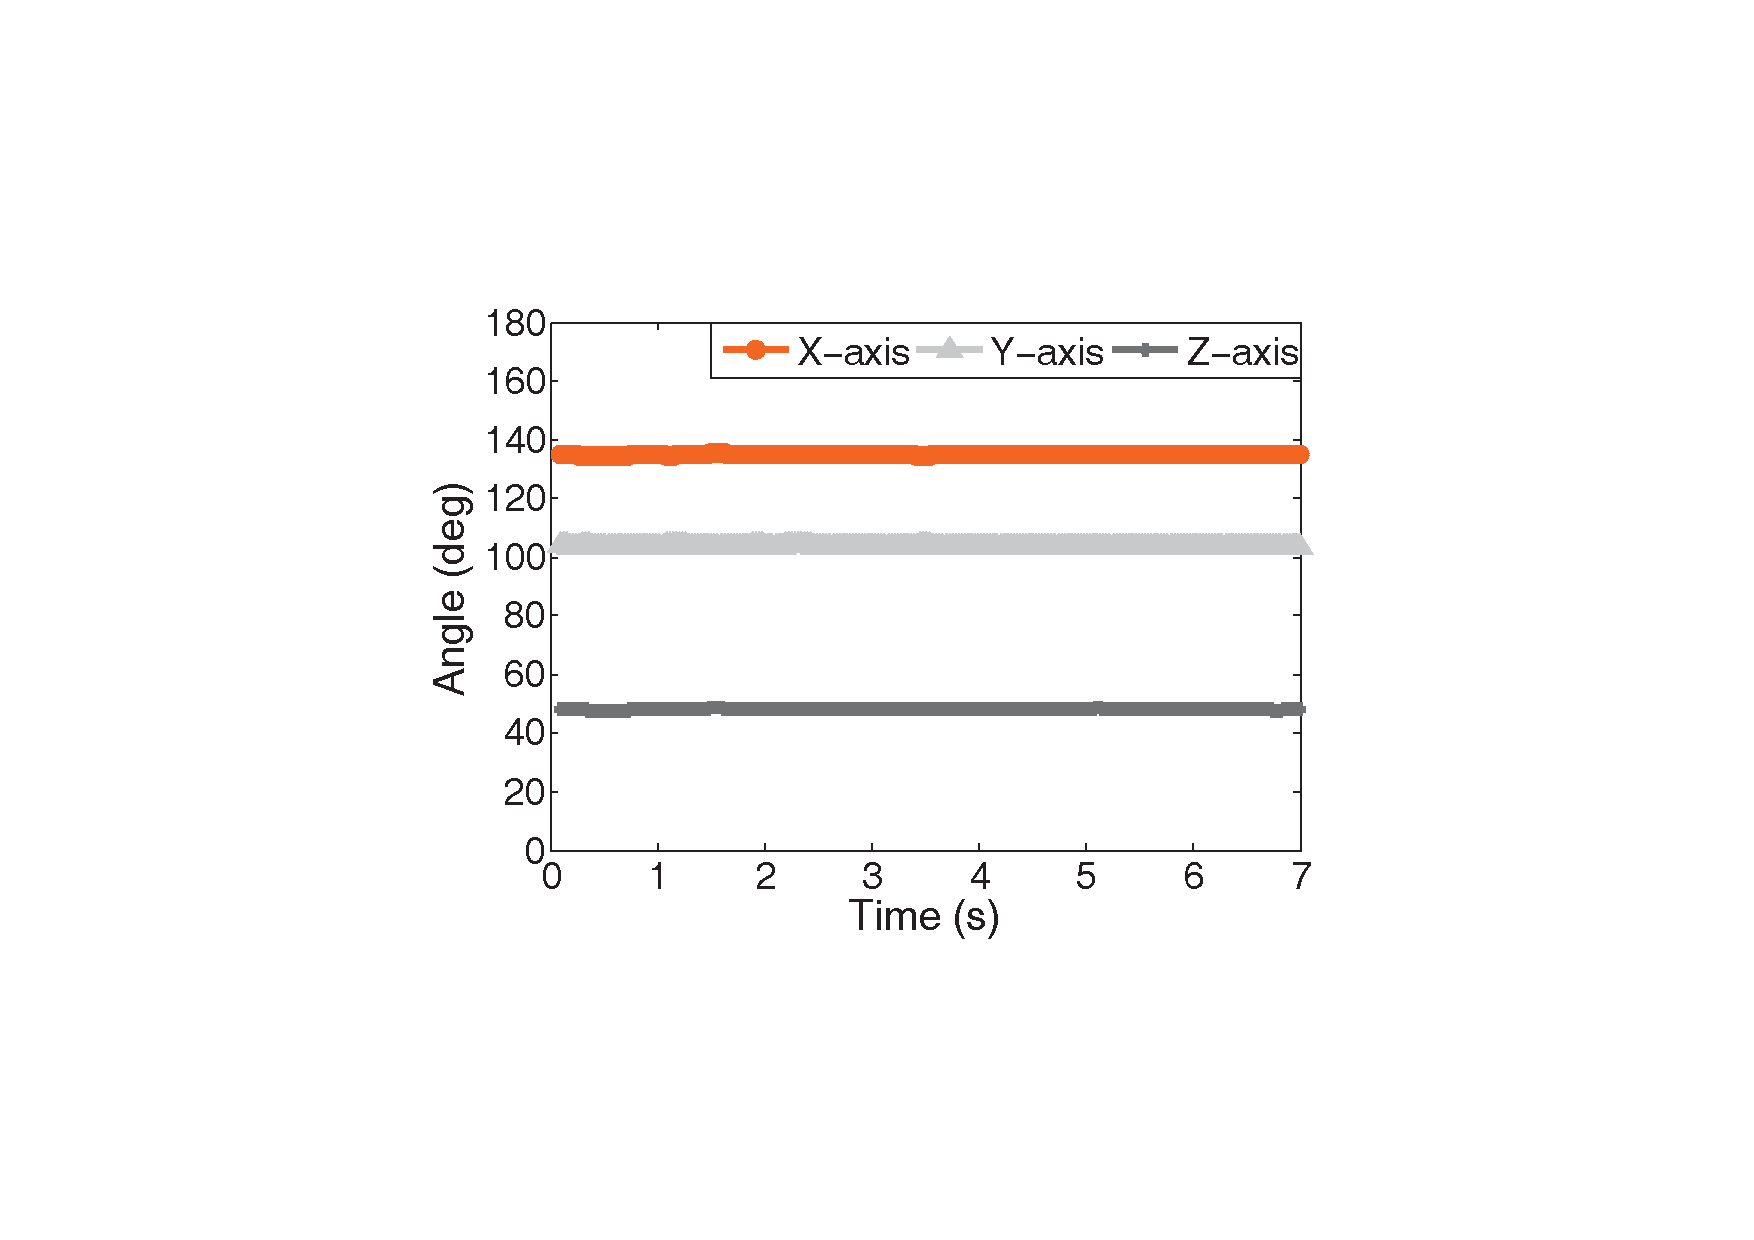
\includegraphics[width=0.24\linewidth]{Figures/RightLateral.pdf}}
	%\hspace{1in}
	\hfill
	\subfigure[Prone]{
		\label{fig:Prone}
		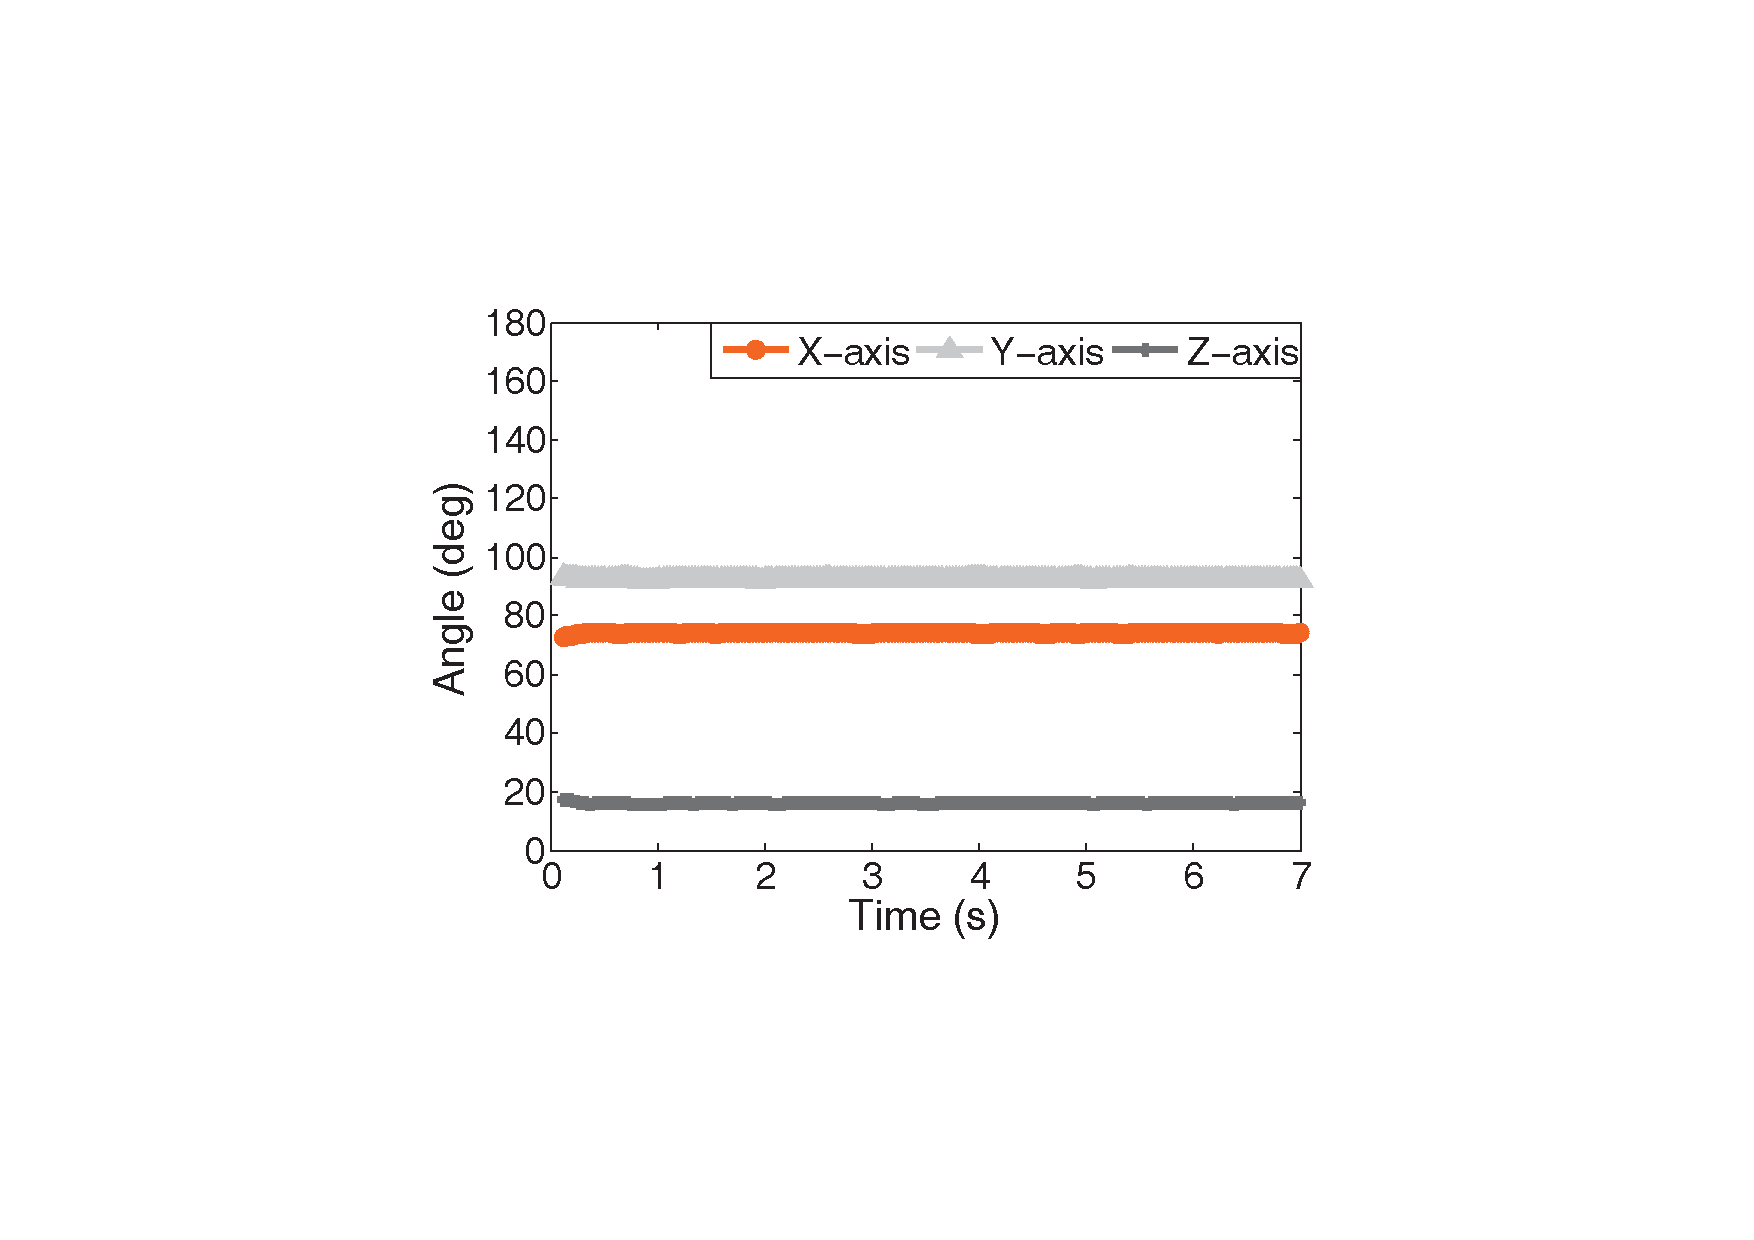
\includegraphics[width=0.24\linewidth]{Figures/Prone.pdf}}
	\caption{The tilt angle characteristics of four body postures.}
	\label{fig:posture}
\end{figure}

%e use a supervised classifier to  And then we use a supervised learning method to create a sleep posture profile. Specifically, we collect training data to create a mapping (i.e., angle mapping) between the angles and the arm under different positions.

Similarly to SleepMonitor~\cite{sleepmonitor}, we use tilt angles readings from three dimensions to detecte postures. We use a K-nearest
neighbour (with $k$ set to 1) classifier to determine which of the targeting postures that a input feature vector corresponds to. To
determine which posture an input feature corresponds to, we find which of the four posture profiles (i.e., a tilt angle value) is closest
to the input data. The posture profiles used for this task are collected from our pilot study involved 10 users who are different from the
ones took part in our evaluation. To identify which of the postures the data collected within a time window corresponds to, we average all
the calculate tilt angle values of that window. To determine which posture an input feature corresponds to, we find which of the four
posture profiles (i.e., tilt angle values in three dimensions) is closest to the input data. The posture profiles used for this task are
collected from our pilot study involved 10 users who are different from the ones took part in our evaluation. To identify which of the
postures the data collected within a time window corresponds to, we average all the calculate tilt angle values of that window in each
dimension. We then calculate the Euclidean distance of the input values to each of the profiles across the three dimensional to find which
profile is closest to the input values. We then use the body posture associated with the nearest neighbor as the detection outcome.




Fig. \ref{fig:posture} shows the angle values of the four sleep postures targeted in this work. This diagram suggests that the tilt angles
of three axes have obvious differences. The sleep posture thus can be inferred based on the position of the smartwatch and the created
angle mapping. However, a limitation of this approach is that the hand positions during supine and prone postures are similar when the hand
is located on the side of the head (Fig. \ref{fig:Supine} and \ref{fig:Prone}), thus the classification accuracy will be affected.

To improve detection accuracy between supine posture and prone postures, \systemname integrates orientation data as auxiliary feature. This is based on the observation that hand directions in the supine and prone positions are different. When the result of the previous step is prone or supine, and the hand is detected to be located next to the body, we combine the tilt angle with three axes data obtained from the direction sensor as a new feature, and classify these postures using a template-based distance matching approach. Specifically, we return the position corresponding to the template with minimum Euclidean distance with current sensor measurements as the user's posture. %Note that when we use the direction sensor, we must limit the pillow orientation remaining unchanged (in the experiment our pillow is placed on the north). In fact, this assumption can be easily satisfied since most people usually have fixed sleep directions.


\subsubsection{Hand Position Recognition\label{sec:handpr}}

The hand position during sleep can disclose potential health problems, and an improper hand position can even result in health issues~
\cite{position2014}. For instance, placing the hand on the abdomen may indicate discomfort whereas placing the hand on the chest can
increase the likelihood of nightmares due to long-term pressure on the heart. Similarly, placing the hand on the head can put excess
pressure on shoulder nerves and cause arm pain as blood flow is restricted. This can lead to eventual nerve damage, with symptoms including
a tingling sensation and numbness \cite{position2014}.


{\systemname} is designed to recognize three common hand positions -- if the hand is placed on the abdomen, chest or head when the user is
in the supine posture, as shown in Fig. \ref{fig:HandPosition}. We have chosen these three hand positions because there are found to be the
most common and representative positions in our pilot study (Section~\ref{sec:implementation}). Our hand position recognition algorithm is
based on sensor data of rotation angles, tilt angles, and respiratory events. It works by first using the rotation and tile angles to
detect if the hand was placed on the head. If the hand was detected to be not put on the head, it then uses the respiratory events and
rotation angles to distinguish the abdomen position from the chest position. We now describe how to detect each of the three positions in
more details.




%\textcolor{blue}{The reason why we choose these three hand positions is that they are found to be the most common and representative
%positions during our pilot study (see Sec. 3.1), and they are really related to sleep and health.} Note that as the hand is mostly on the
%bed in prone and lateral positions, the main benefits of hand position recognition are for detecting the supine posture.

\paragraph{Detect the head position.}
Fig.~\ref{Bodyhand} show the rotation angle values gathered from the x, y, and z dimensions using the gyroscope for one of our pilot study
users when his hand next to the body was moved to his head, abdomen, and chest. It is to note that we also observe similar behaviors for
our other participants. As can be seen from the figure, when the hand is moved to the head, the changes in the rotation angles are
significantly different from the readings given by moving the hand to the abdomen and the chest. This is largely due to the different
direction that the palm is facing when the hand is placed on the head compared to the other positions.  \systemname exploits this
observation to detect if the hand is placed on the head by inspecting the changes of the rotation angles and the hand trajectory.
Specifically, ....

%We have designed a novel algorithm to map hand trajectories to  hand positions. The key intuition behinds our algorithm is that any change
%in hand position results in a movement trajectory that is uniquely determined by the start and end position of the hand. By comparing
%motion measurements with such hand trajectory profiles, we can identify the most likely position. Like posture detection, we also use a
%K-nearest neighbor classifier to recognize the hand position. In \systemname we consider nine different types of hand trajectories,
%corresponding to motions from the side of body to the chest, head or abdomen, and those between head, chest and abdomen. Note that we do
%not consider the case where the hand moves from head, chest, or abdomen to the side of the body as this is established as part of the
%posture classification.

\begin{figure}[!t]
	\centering
	%\begin{minipage}[t]{0.325\linewidth}
    	\subfigure[moving to the head]{\label{BodytoHead}
		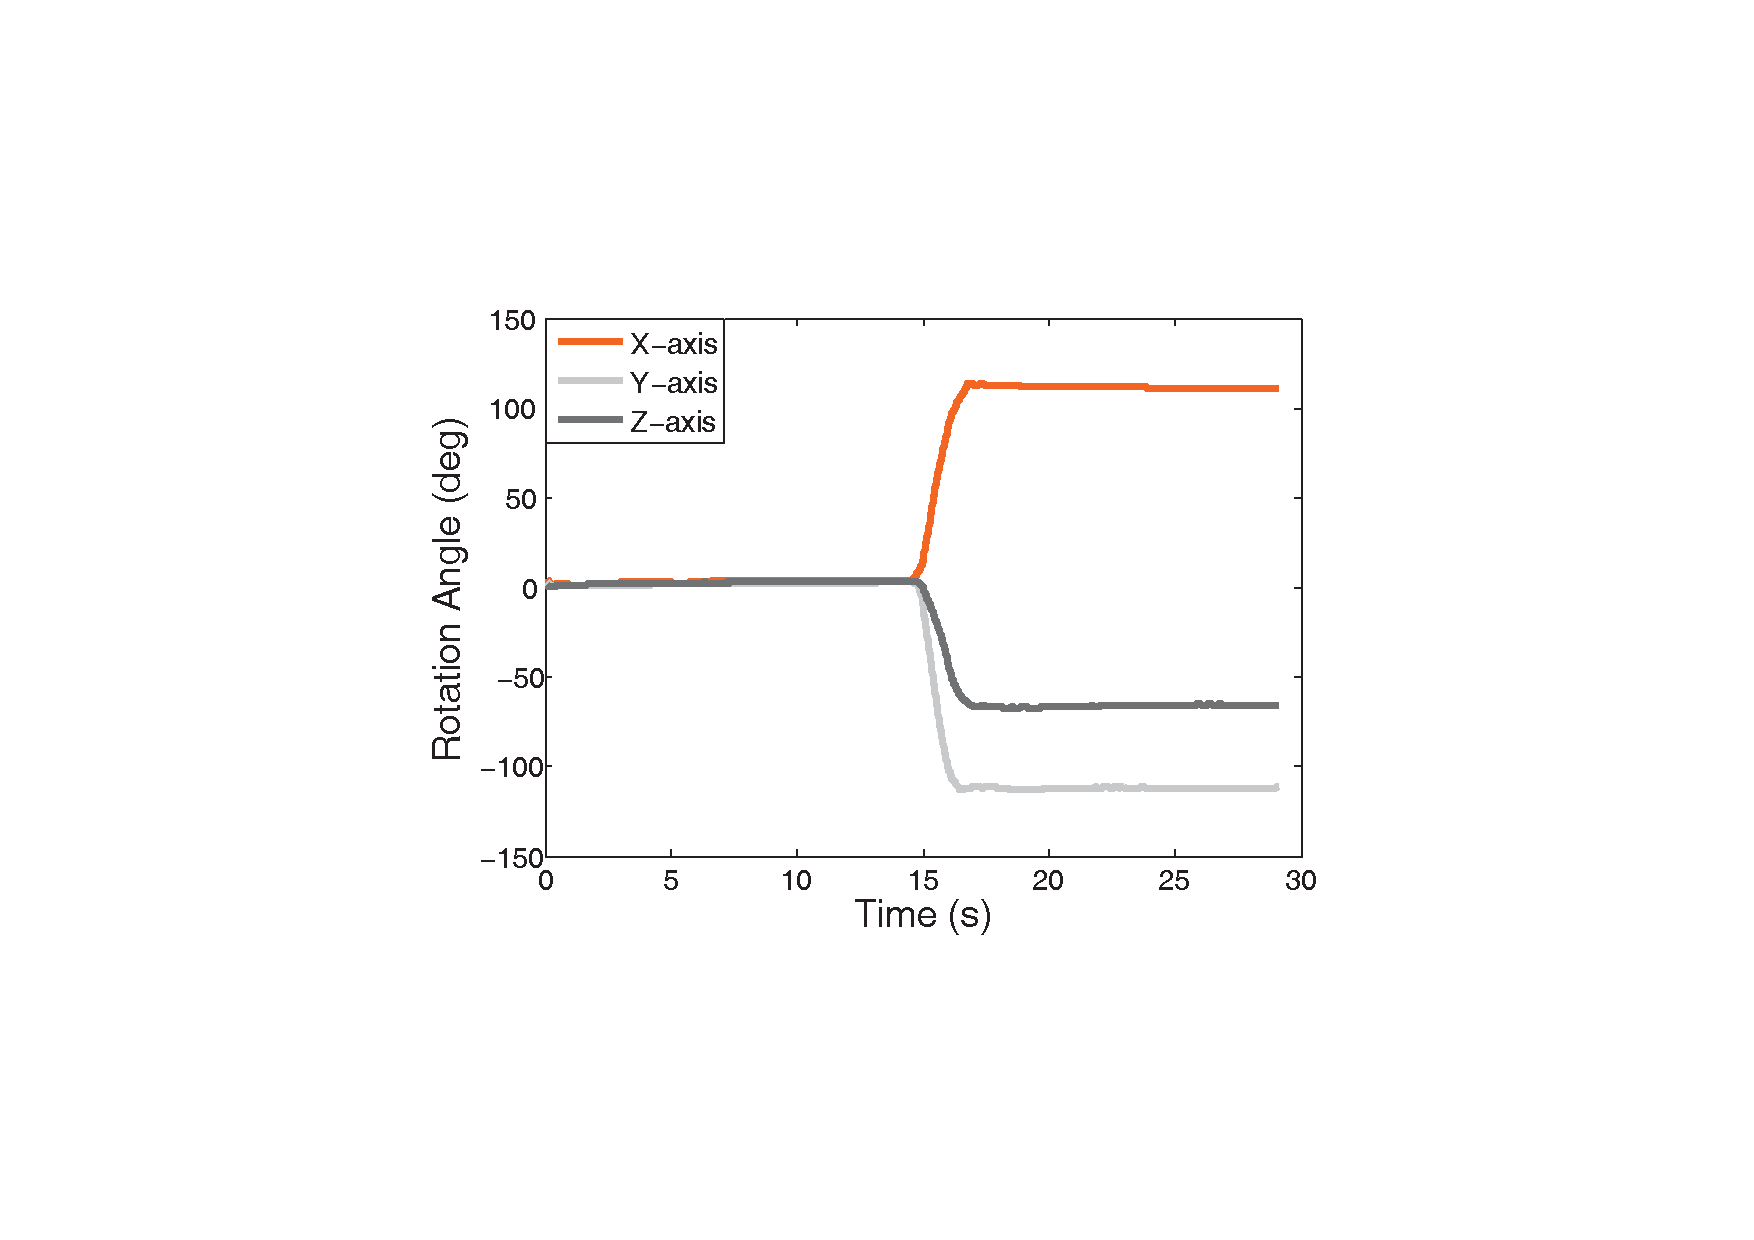
\includegraphics[width=0.32\linewidth]{Figures/BodytoHead.pdf}}
	\subfigure[moving to the abdomen]{\label{BodytoAbdomen}
		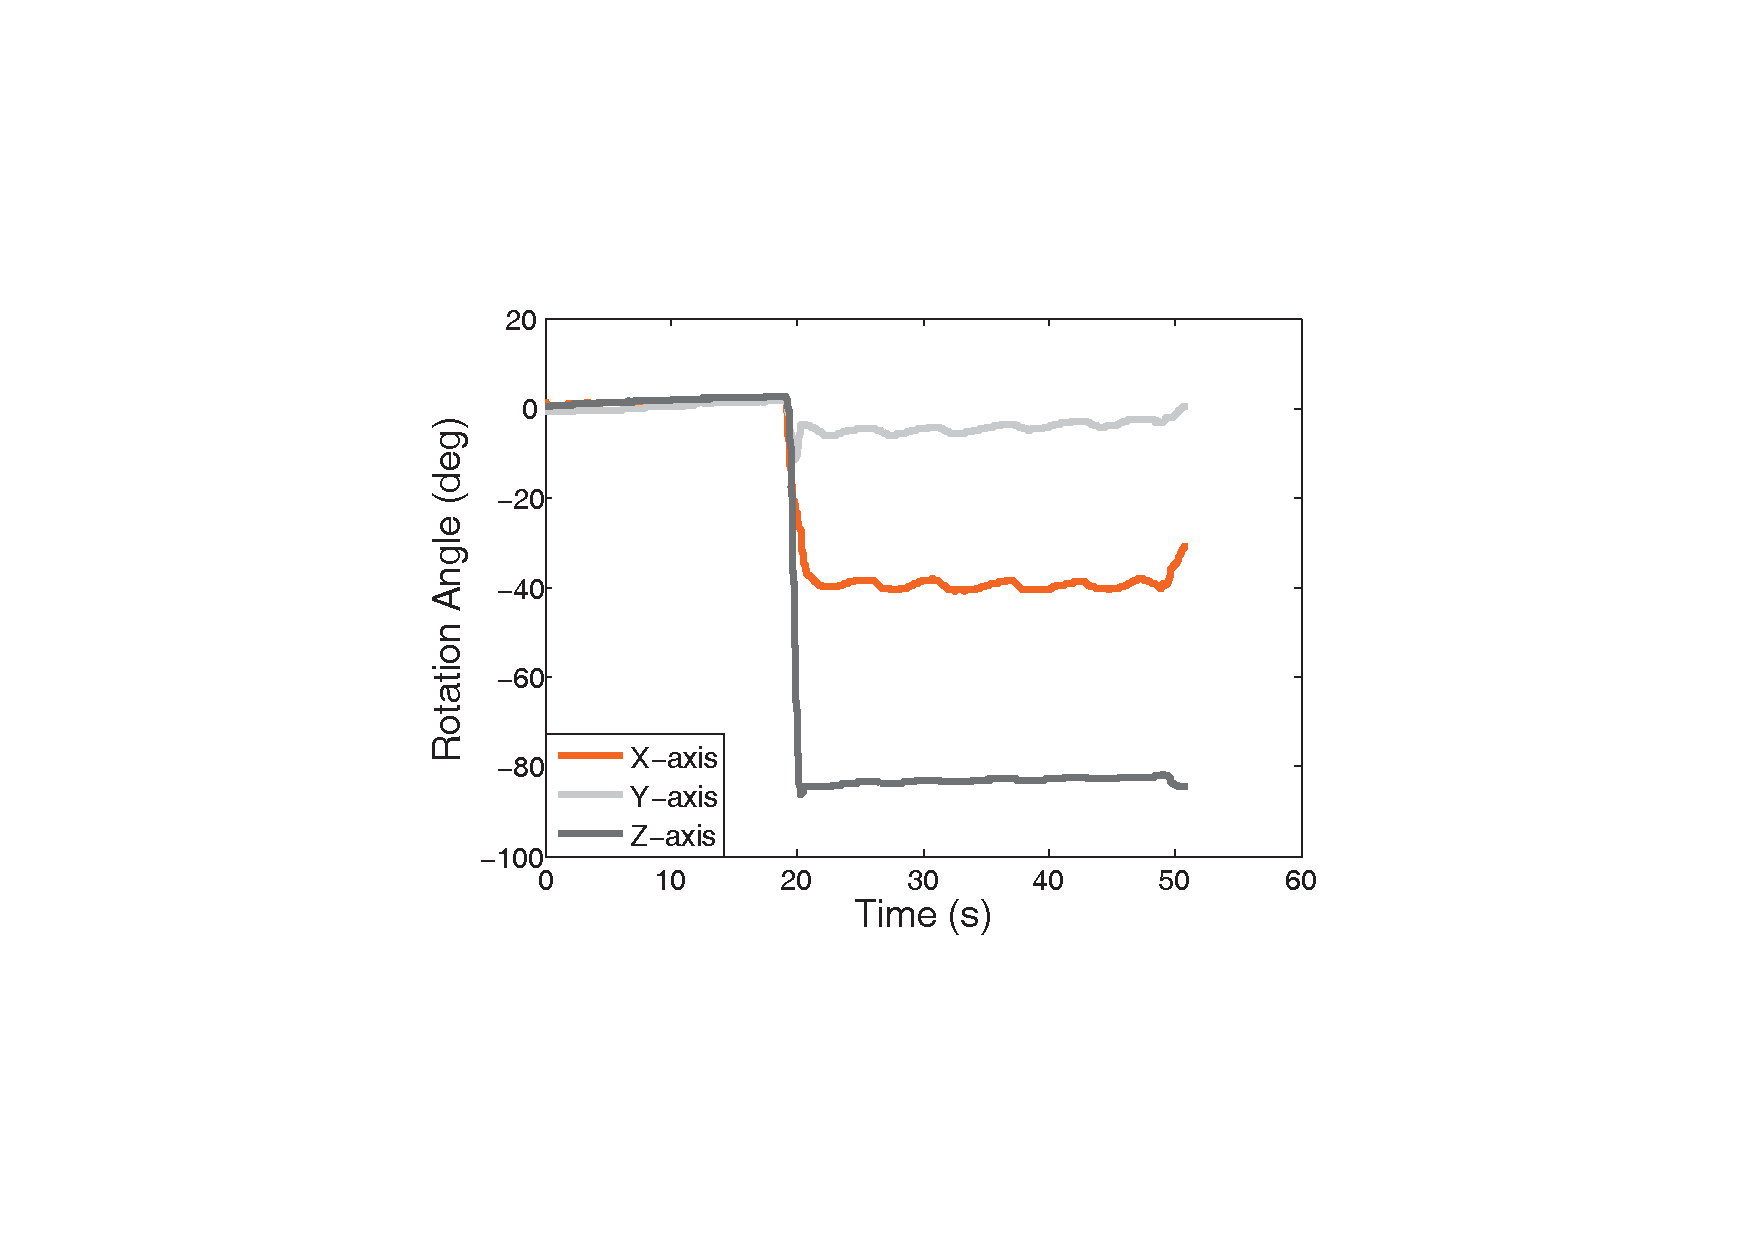
\includegraphics[width=0.32\linewidth]{Figures/BodytoAbdomen.pdf}}
	%  \hfill
	\subfigure[moving to the chest]{\label{BodytoChest}
		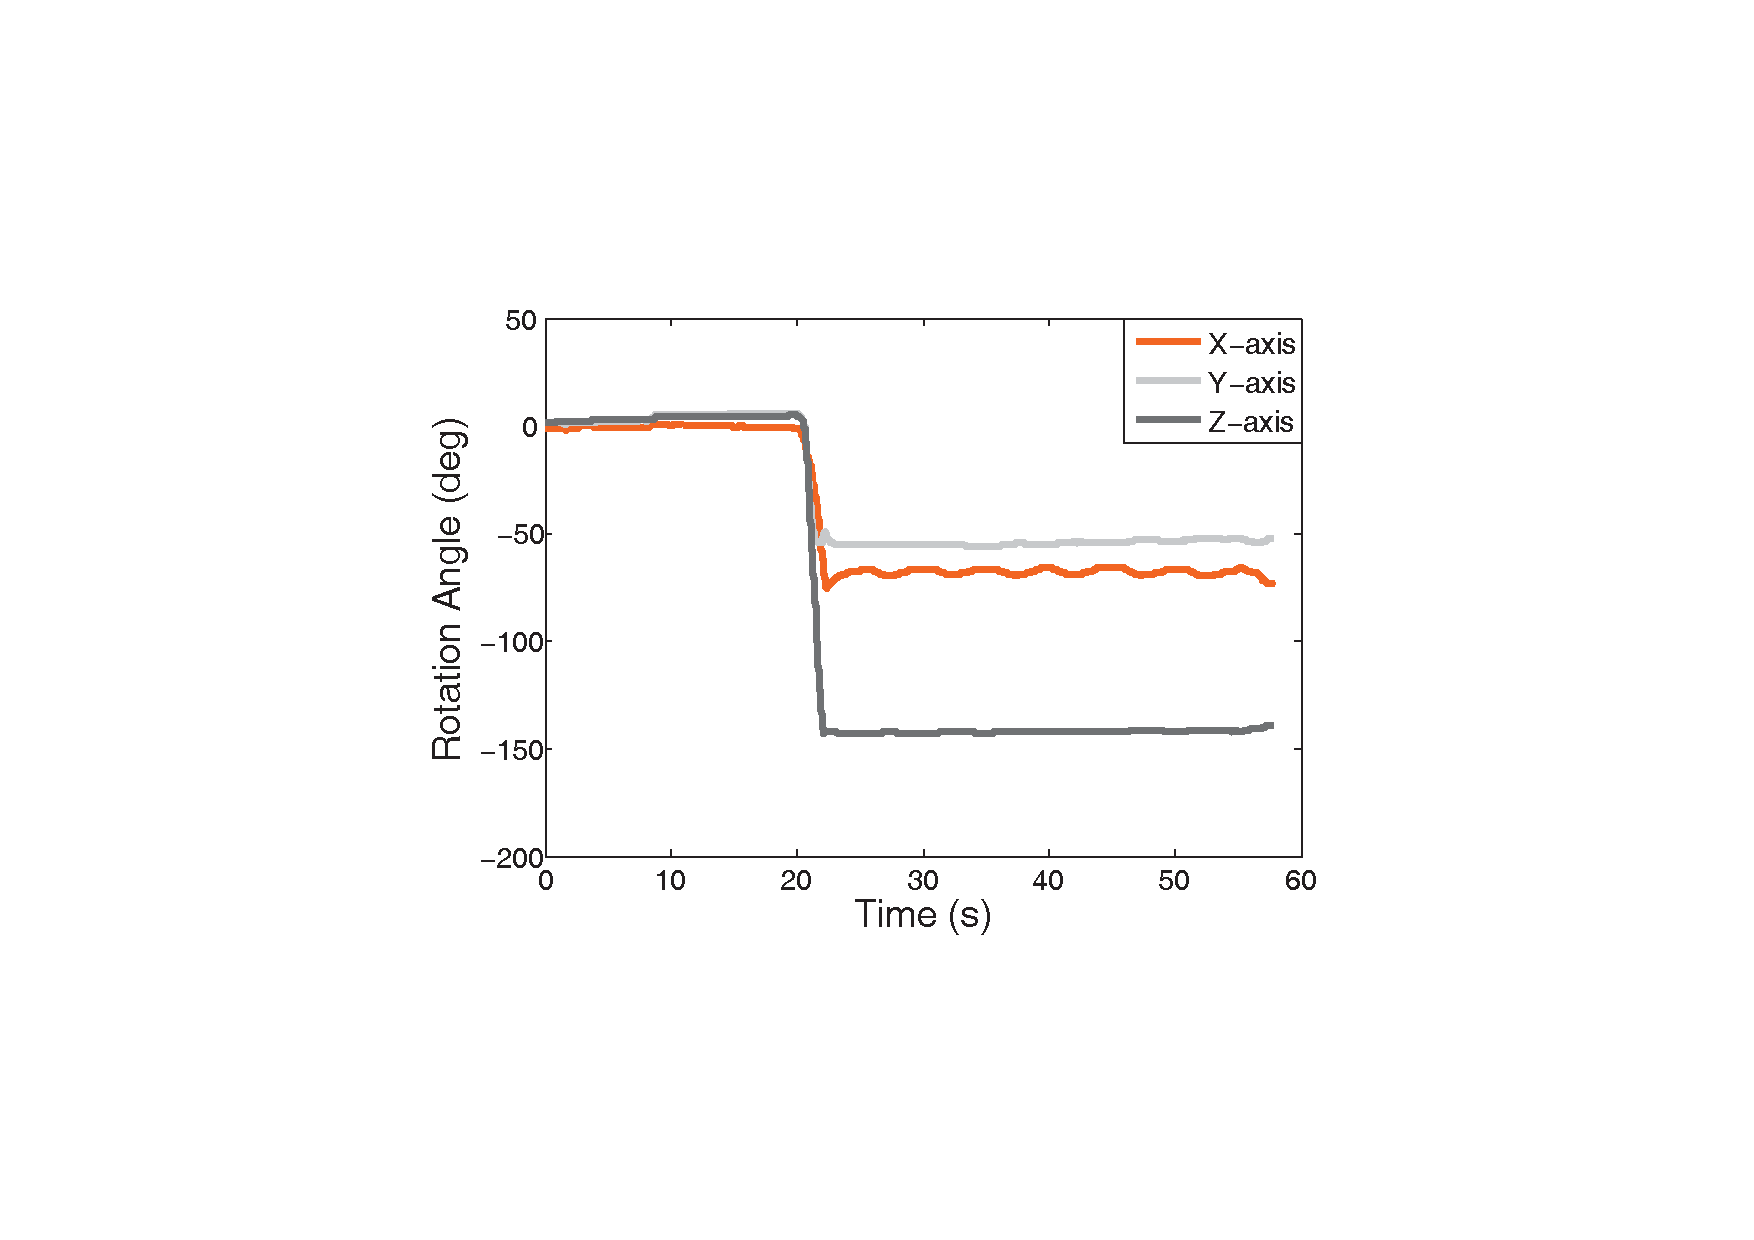
\includegraphics[width=0.32\linewidth]{Figures/BodytoChest.pdf}}
	%  \hfill
  %  \subfigure[moving to the shoulder]{\label{BodytoShoulder}
%		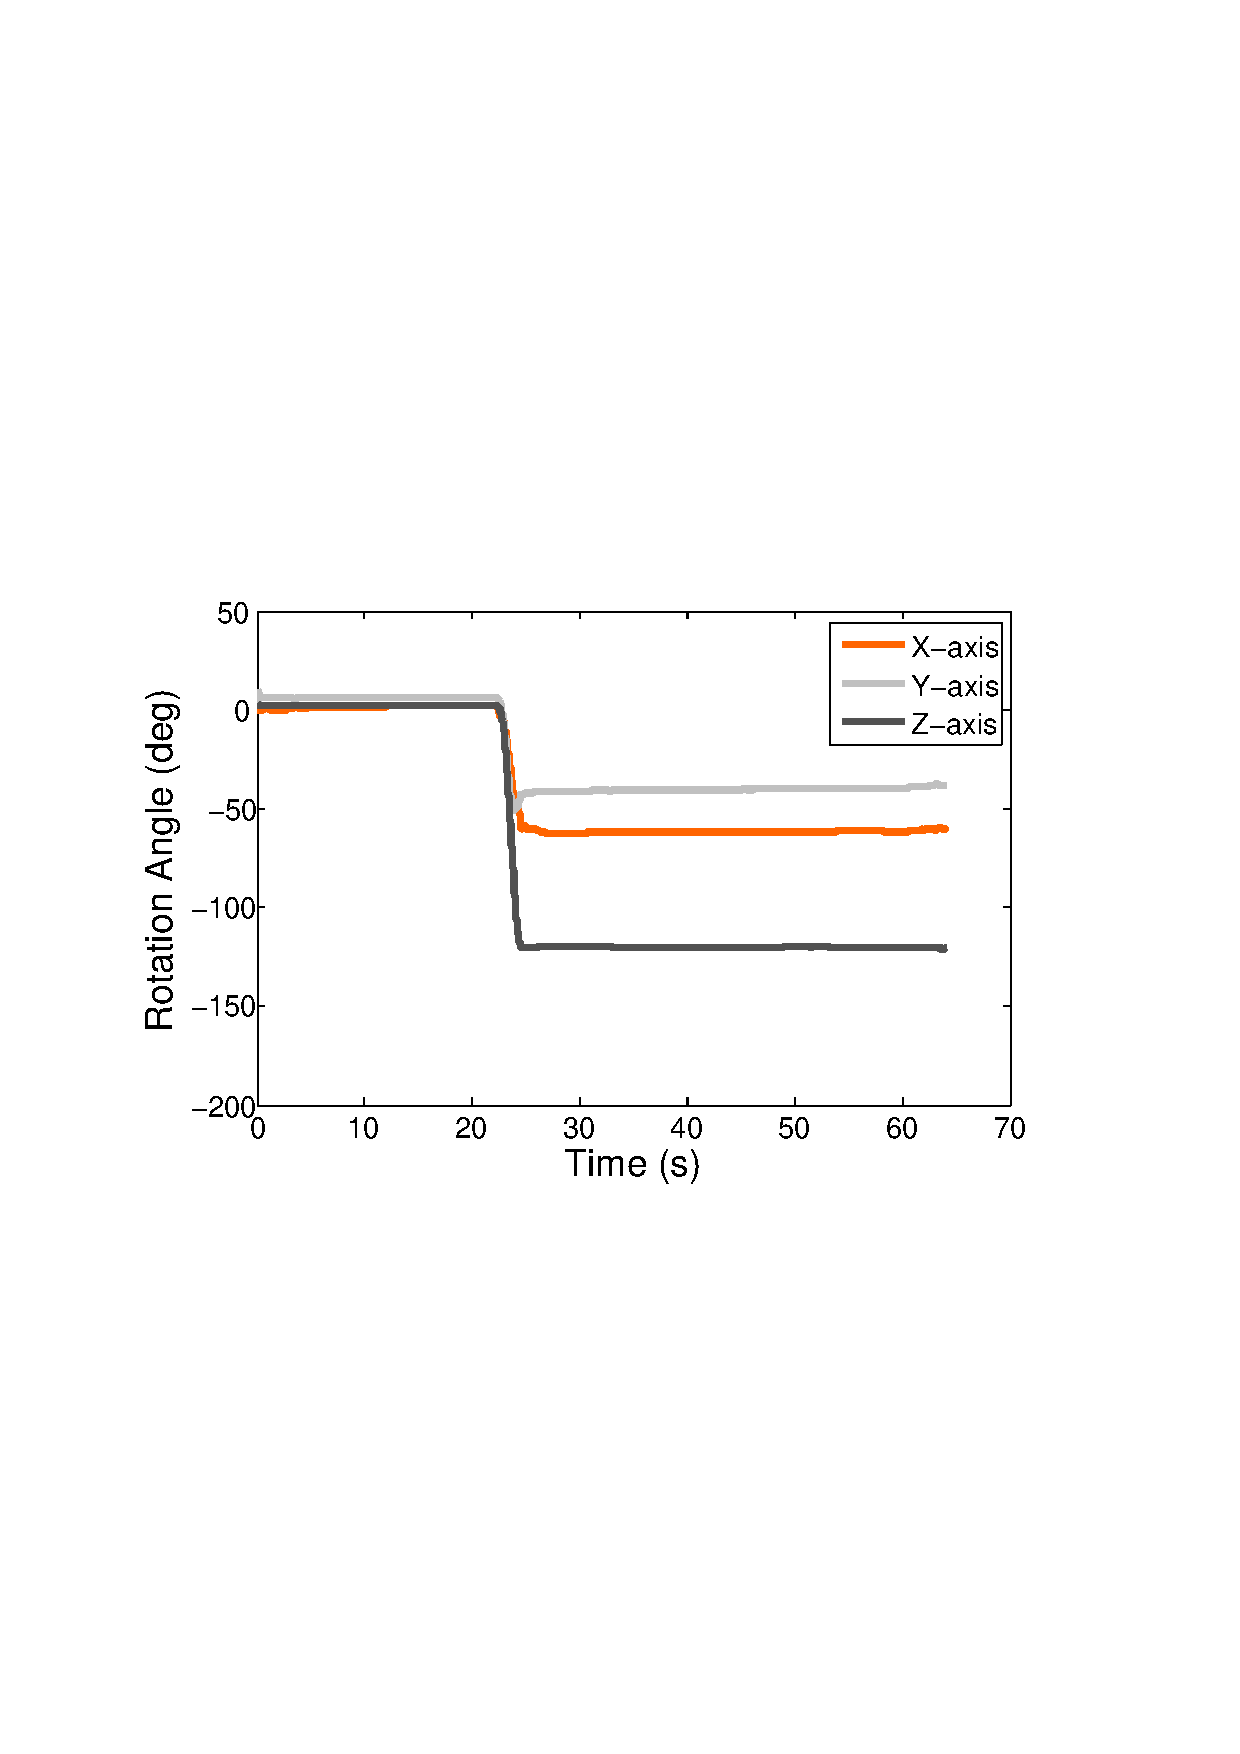
\includegraphics[width=0.34\linewidth]{Figures/BodytoShoulder.pdf}}
	\caption{Rotation angle values when a hand of one of our users, placed next to the subject's body, is moved to his head (a), abdomen (b), and chest (c). }\label{Bodyhand}
\end{figure}

\begin{figure}
	\centering
	\begin{minipage}[t]{.475\textwidth}
	\centering
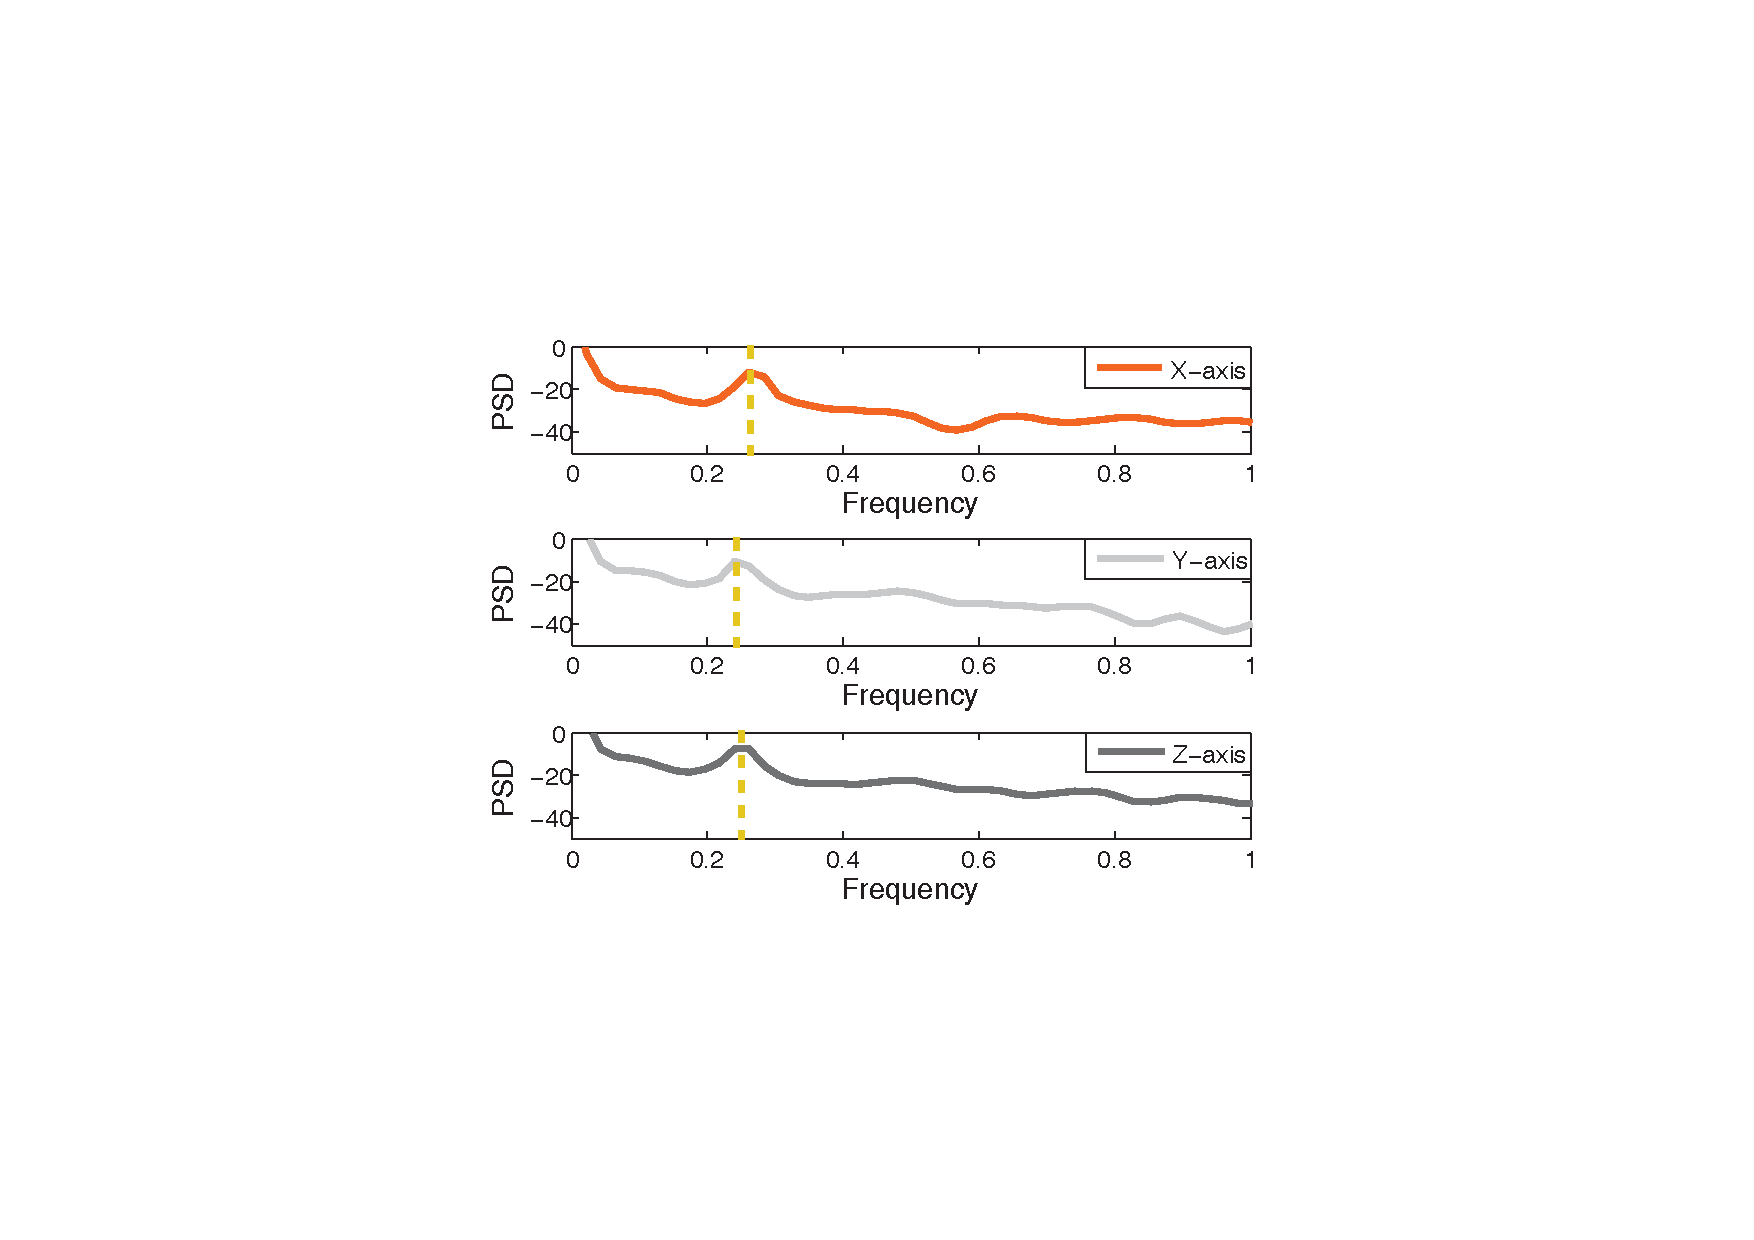
\includegraphics[width=7cm,height=5cm]{Figures/PSD.pdf}
\caption{The power spectral density (PSD) of the acceleration signal.}\label{fig:PSD}
	\end{minipage}%
\hfill
	\begin{minipage}[t]{.475\textwidth}
	\centering
	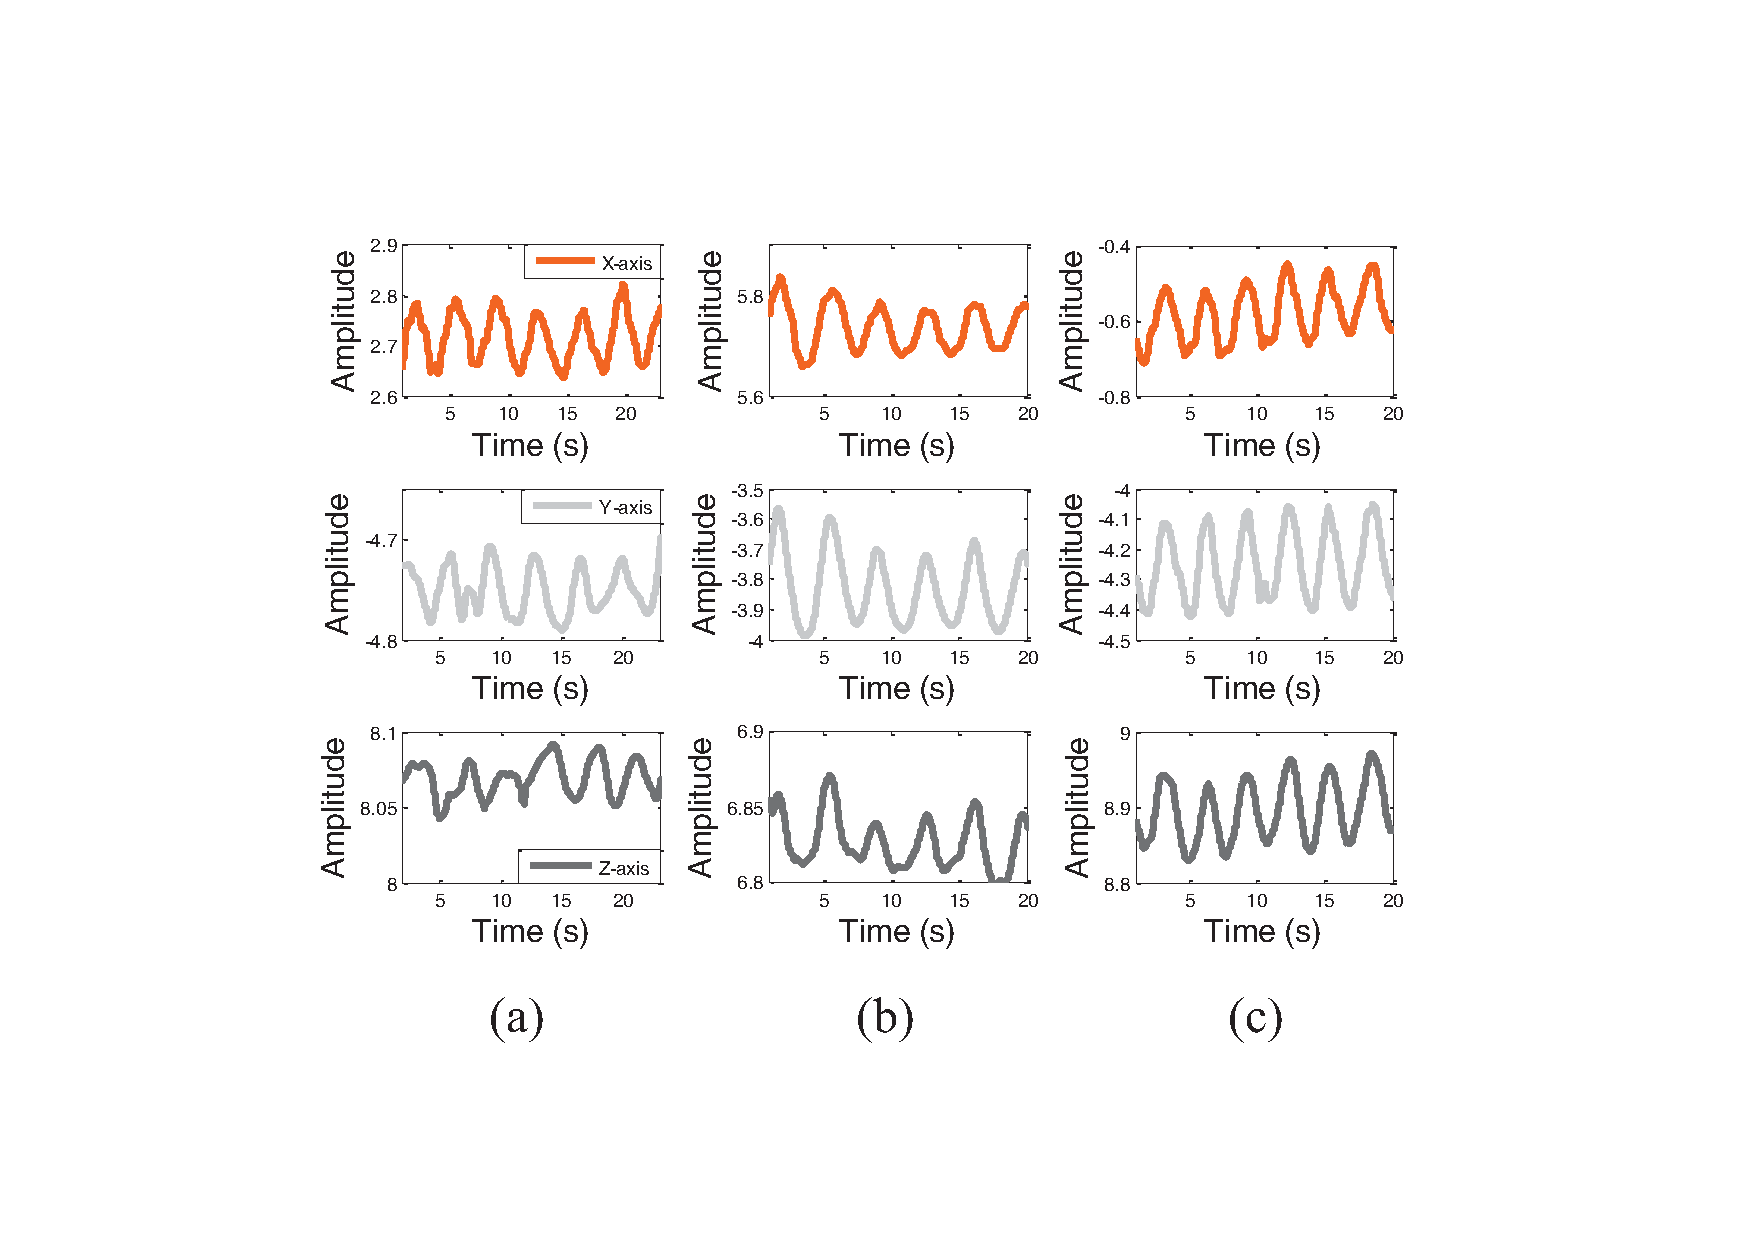
\includegraphics[width=7cm,height=5cm]{Figures/breath_ok1.pdf}
	\caption{The periodic change of the acceleration signal. (a) REM--Location 1. (b) REM--Location 2.  (c) NREM--Location 1.}\label{fig:breath_ok1}
	\end{minipage}
\end{figure}

%result in uniquely identifiable trajectories that are specified by the start and end point of the hand. By comparing information about the latest trajectory against movement templates (analogously to

%that we can identify current hand position by analysing the latest hand trajectory which caused the hand position to change. we have developed a novel algorithm that is based on the key intuition that, before the hand is placed on the body, it experiences a movement from side of the body to the end position, and after that the hand always experiences a movement from one position to the other. Thus we can further integrate the hand movement trajectory to determine the hand position at current time. In {\systemname}, We consider nine kinds of the trajectories of hand, from the side of the body to the abdomen, to the chest, to the head; from the chest to the abdomen, to the head; from the abdomen to the chest, to the head; from the head to the abdomen, to the chest.
Fig.~\ref{Bodyhand} shows the rotation angle changes in three dimensions (x, y and z), when the hand next to the body is moved to different
parts of the body. The data are collected using the gyroscope. To aid clarity, we present the data collected from one of the users
participated in our pilot study, similar behaviors are observed for all other participants. \textcolor{blue}{In the picture, we only show
the signals from a single subject. This is because after experiments we found that the three hand trajectories of the hand are roughly the
same in different people. We only show the approximate relative trend to indicate that the difference in the hand trajectory. So we can use
the three-axis rotation angle calculated by the gyroscope as a feature to establish a sample library, and use the template distance
matching classifier to identify the final position of the hand. However, if we only use the hand's movement trajectory to determine the
position of the hand, then we only get the movement relative to a certain known starting position, not the final absolute position of the
hand. That is, only when we know that each time the starting position of the hand before movement, we can judge the final hand position
based on different trajectories. However, in practical applications, it is difficult for us to obtain the starting position of the hand
every time. Therefore, we only cannot rely on the hand movement trajectory to achieve the purpose of detection. However, we found that when
the hand is placed on the head, the hand placement is clearly different from that of the hand on the chest or abdomen, which makes it
easier to detect by the angle characteristics calculated by the acceleration when placed on the head. When the hand is on the chest or
abdomen, the angle characteristics are very similar and difficult to distinguish. Hence, we need an additional verification step to ensure
the hand is on the chest or abdomen. We can based on key intuition is that we can observe acceleration signals to exhibit a distinctly
periodic fluctuation, as shown in Fig. \ref{Bodyhand}. This is due to the movement of the abdomen and chest caused by breathing. Therefore,
we can use the occurrence of respiratory events to determine if the hand is indeed on the body (abdomen or chest). Through the detection of
respiratory events, we can not only determine the initial position of the hand before movement but also filter out some areas near the
chest or abdomen, such as the shoulders or hips. This is because when the hand move to the shoulder or hip and some other areas close to
the chest or abdomen, the resulting hand trajectories are very similar, but we can not observe significant respiratory events, as shown in
Fig. \ref{BodytoChest} and Fig. \ref{BodytoShoulder}. So we can combine with the hand's
movement trajectory to accurately determine the hand position.}%This results in a rough classification that determines situations where the
hand is in the vicinity of one of the targeted positions. However, depending on the trajectory, we cannot be sure that the hand is exactly
in the chest or abdomen. This is because when the hand move to the shoulder or hip and some other areas close to the chest or abdomen, the
resulting hand trajectories are very similar. Hence, we need an additional verification step to ensure the hand is on the chest or abdomen.
The key intuition for separating these cases is that we can observe acceleration signals to exhibit a distinctly periodic fluctuation, as
shown in Fig. \ref{Bodyhand}. This is due to the movement of the abdomen and chest caused by breathing.Therefore, we can use the occurrence
of respiratory events to determine if the hand is indeed on the body (abdomen or chest).
 Specifically, we calculate the power spectral density (PSD) of the acceleration signal, where the highest peak frequency is the signal's frequency. From Fig. \ref{fig:PSD}, we can see that there is a large peak located at around 0.25 Hz, which corresponds the respiratory frequency. \textcolor{blue}{So if the signal's frequency falls within the reasonable breathing frequency range, it indicates the occurrence of respiration events, that is, the hand is put on the chest or abdomen. According to our survey\cite{Breath_frequence}, an adult's normal breathing frequency averages about 15 times per minute. As the age decreases or increases, the frequency of breathing increases. So we detect the occurrence of respiratory events using a threshold range of 12 times (0.2 Hz) per minute to 28 times (0.47 Hz) per minute. This is a reasonable range based on some prior research work and our observation. }

In addition, we found that the extent of body movements can be used to judge the amplitude of respiration. What's more, we know that when people sleep in the REM stage, their respiratory amplitude is smaller than in the other stages~\cite{respiratory1982}. Hence, we can roughly determine the user's current sleep stage based on the respiratory amplitude. Respiratory amplitude is only an indicator of the division of the sleep stage and we can not regard it as a basis for final judgement, but it serves as an early reference that helps later phases of the sleep stage detection. Under normal circumstances, the chest movement amplitude is smaller than abdominal movement amplitude. However, in different sleep stages, the respiration amplitudes are different~\cite{respiratory}. It is likely that there is a situation: the chest movement amplitude in the NREM stages is close to the abdominal movement amplitude in the REM sleep stage. As a result, the threshold based method cannot work. At this time, we need to combine it with the position of the hand we detected with the trajectory before. Through the above steps, we have been able to determine whether the hands are on the chest or abdomen, and then we can go further to determine the extent of breathing according to the degree of body ups and downs, and we can roughly infer the sleep stage. Now we take the case of hands on the abdomen as an example.



Even when the hand is placed on the abdomen, due to minor changes in the exact location of the user's hand, the location of intensity of accelerometer fluctuations caused by respiration varies. Hence, we cannot use the amplitude information to determine true respiratory amplitude directly. This problem is illustrated in Fig.~\ref{fig:breath_ok1}, where (a) and (b) contain triaxial acceleration measurements at different locations of the abdomen during REM sleep stage, and in (c) which consists of acceleration data for NREM stages at the same approximate position as in (a). We can see that when hand on the abdomen, but the location is different, even in the same location, we can not directly judge the respiration amplitude using only the amplitude of the three axes of the acceleration.

\begin{figure}[!t]
\centering
      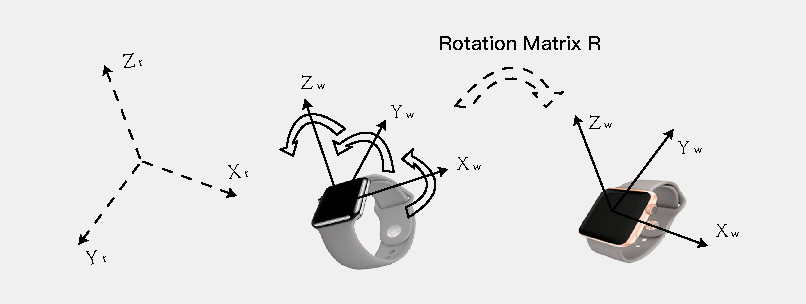
\includegraphics[width=0.67\linewidth]{Figures/watch.pdf}
  \caption{The first figure on the left is the torso coordinate system, and $Y_t$ points north. The middle figure shows the watch coordinate system when the watch an arbitrary position, and the right of the figure shows that the  watch coordinate system after we completed the coordinate system conversion.}\label{fig:watch}
\end{figure}

To solve this problem, we convert the acceleration data from the wristwatch coordinate system into the data in the torso coordinate system. Because we can know that when the person is in the supine position, the abdomen and the chest will move up and down due to breathing, that is, move along the z-axis direction of the torso coordinate system. We express the triaxial acceleration data as $Acc_w$ = [$X_w$, $Y_w$, $Z_w$] in the wristwatch coordinate system and $Acc_t$ = [$X_t$, $Y_t$, $Z_t$] in the torso coordinate system, as shown in Fig. \ref{fig:watch}. And the watch coordinate system ({[$X_w$, $Y_w$, $Z_w$]}) is determined by the position of the watch. Our coordinate alignment aims to find a rotation matrix R to align the watch's coordinate system to the torso coordinate system ({[$X_t$, $Y_t$, $Z_t$]}) and R can be obtained by the three-axis direction information in the orientation sensor. After the coordinate system is aligned, the angle between the y-axis of the wristwatch coordinate system and the y-axis of the torso coordinate system is 180 degrees.
\begin{equation}
      X_t  = (X_w {\cos\gamma} + Y_w{\sin\gamma}){\cos\theta} + (Y_w\cos\sigma + Y_w\sin\sigma)\sin\theta,
\end{equation}
\begin{equation}
      Y_t = -((Y_w\cos\sigma + Y_w\sin\sigma)\cos\theta - (X_w\cos\gamma + Y_w\sin\gamma)\sin\theta),
\end{equation}
\begin{equation}
      Z_t = (Z_w\cos\gamma - Z_w\sin\gamma)\cos\sigma - (Z_w\cos\gamma - Z_w\sin\gamma)\sin\sigma,
\end{equation}

$\theta$, $\sigma$ and $\gamma$ are the x, y and z axis data of the orientation sensor respectively, representing the direction angle, the tilt angle and the roll angle collected from the orientation sensor. After the alignment of the coordinate system, we can see from Fig.~\ref{fig:cordi} that the z-axis shows a periodic signal with significant fluctuations, while the x- and y-axis data undergo smaller changes around zero, which is consistent with the actual situation that when the person is in the supine posture with the abdomen up and down caused by respiratory.

 \begin{figure}[!t]
\centering
      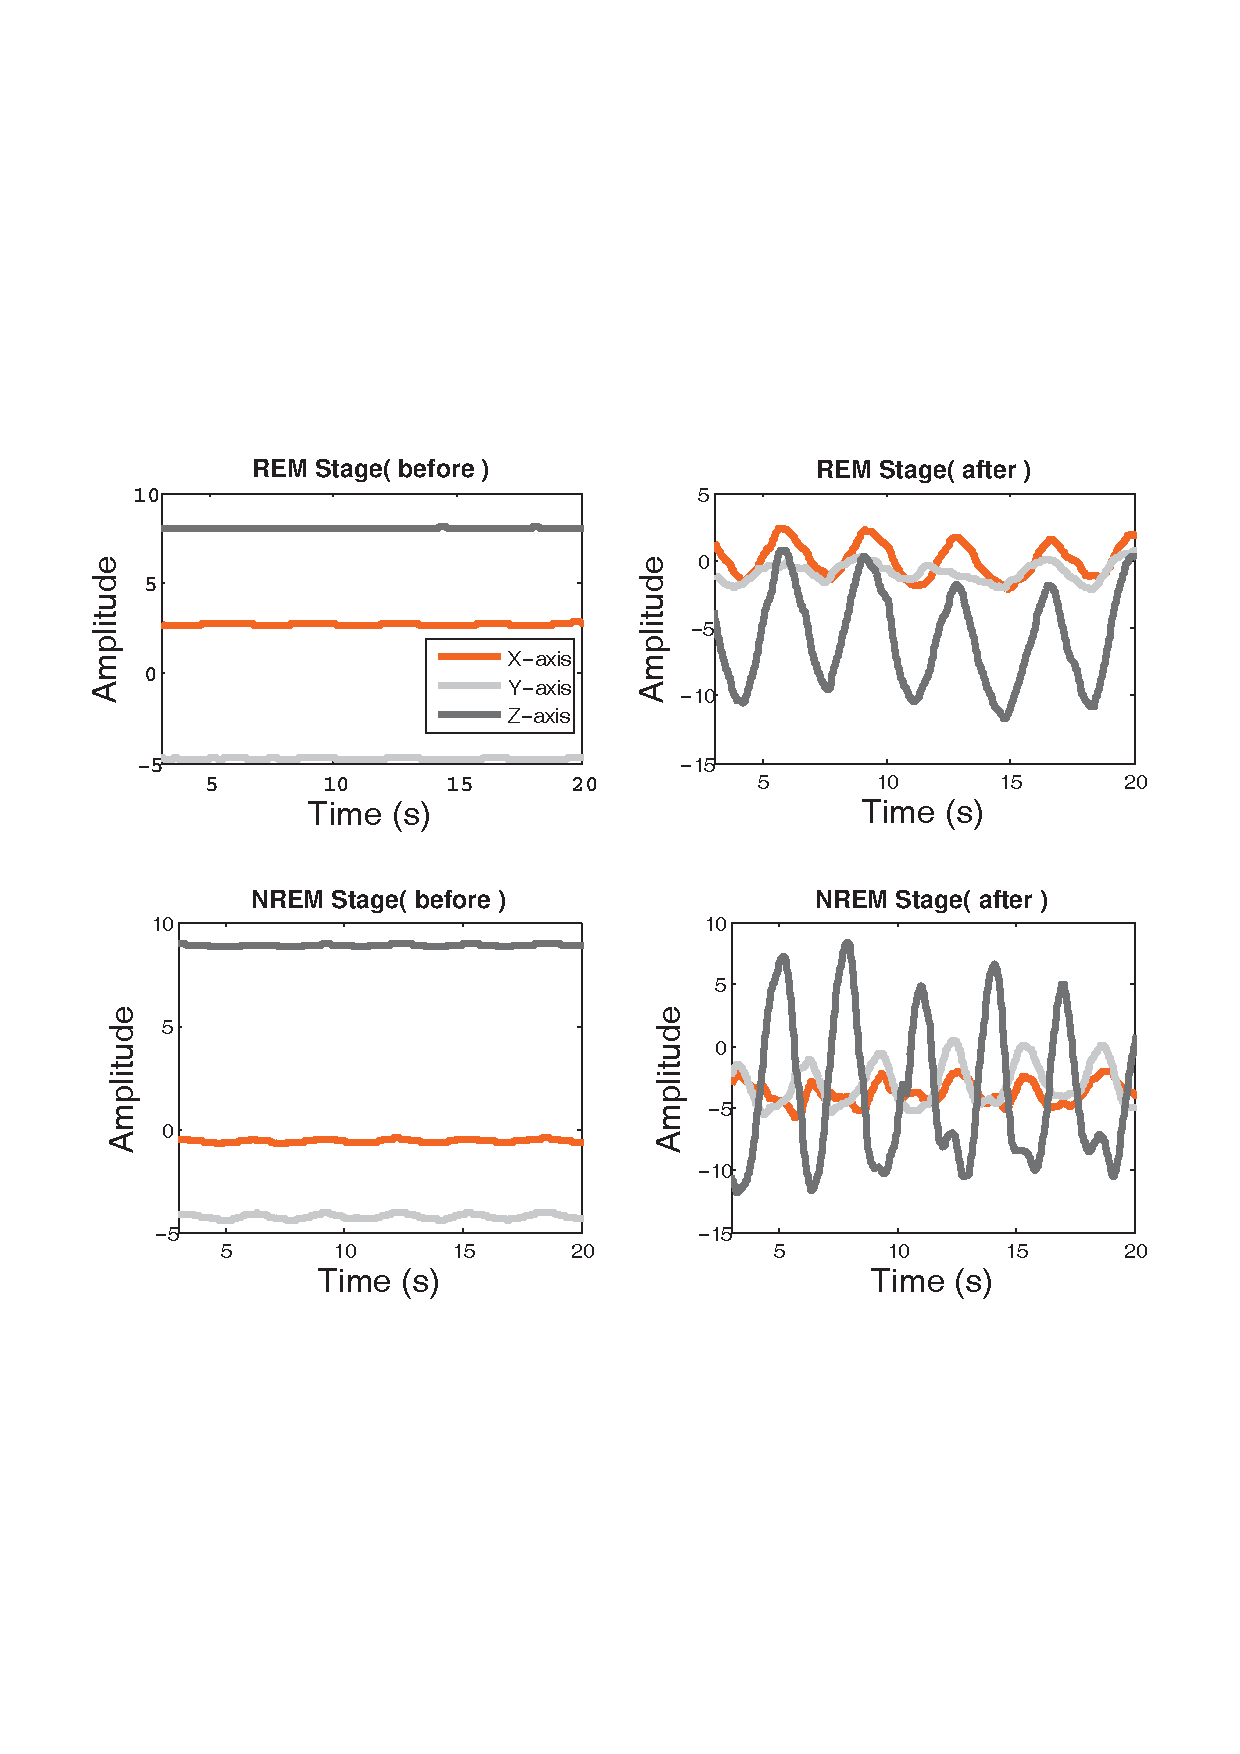
\includegraphics[width=0.75\linewidth]{Figures/cordi.pdf}
  \caption{Acceleration data for different sleep stages.}\label{fig:cordi}
\end{figure}

The two graphs on the left of Fig.~\ref{fig:cordi} show the same acceleration data as has been used in (a) and (c) of Fig.~\ref{fig:breath_ok1}, respectively, whereas the two right-most graphs correspond to the data after coordinate system alignment.  We can see that prior to align the measurements, we cannot effectively distinguish respiratory amplitude of REM and NREM stages from the acceleration amplitude. After coordinate alignment, the respiratory amplitudes are clearly visible from the z-axis data. We then calculate the variance of z-axis acceleration and use it as a feature to measure the intensity of the fluctuation in a signal, with larger variance corresponding to greater breath amplitude. Note that we cannot use the sum or magnitude of the z-axis as a measure of intensity as the measurements remain affected by gravity. \textcolor{blue}{We then trained a classifier based k-nearest neighbor model (with k = 1) using this feature when the hand is placed on the abdomen and on the chest under both REM stage and NREM stages to determine a mapping from current respiratory amplitude to placement. Here, we define the respiratory amplitude in the NREM stage as large respiratory amplitude, and the respiratory amplitude in the REM stage as normal respiratory amplitude. As for the acquisition of sleep stage, we confirm the label of it when both Fitbit and {\systemname} reach a consensus. At the same time, We also take into account video recorded by the camera to manually label part of the respiratory. The combination of these three kinds of equipment can enable us to obtain real and accurate data as much as possible.  As classifier we used a decision stump which was trained on 200 sets of acceleration data (100 sets of these from the larger respiratory amplitude and the rest of sets from the normal respiratory amplitude ) from 10 volunteers, who are randomly recruited by us aged 16 to 60 years old. They are asked to wear a smartwatch to sleep so that we can collect sensor data during sleep. Every volunteer contributes 10 nocturnal sleep data. And we also use these 100 sets of nocturnal sleep-related data as training data for the parameters in our other detection algorithms to enable us get these parameters. The resulting threshold for the acceleration variance is around 15 when the hand on the abdomen, and around 4 when the hand is placed on the chest.}



\subsubsection{Body rollover counts \label{sec:bodyrollover}}

Under normal circumstances, people usually rollover their body around 20-45 times a night. The main function of body rollovers is simply to maintain a comfortable sleeping position as maintaining the same position for prolonged period will result in muscular tension due to hindered blood supply, which can also lead to local numbness~\cite{rollover2014}. So body rollover is another key indicator about the sleep quality. {\systemname} can detect the number of body rollovers, which can get some reflections of sleep status and the roll-over frequency can also help us to classify the sleep stage~\cite{rollover2007}. In general, there are six cases: four posture transition cases between the supine posture and lateral (left or right) posture, and two posture transitions between the left lateral posture and right lateral posture. Fig. \ref{fig:BodyRollover} shows the case when the body moves from the left side to the right side. \textcolor{blue}{The most intuitive way to detect the body rollover events is to detect the direction of rotation of the arm (the rotation angle measured by the gyroscope). However, there is a big drawback to this method. In the actual sleep process, the trajectory of the arm is very difficult to be predicted, especially for different users, and even if there is a slight difference in the starting position of the same sleeping position, it will cause the rotation angle to change and it is easy to cause misjudgment, so this method is not feasible. Therefore, we need to find a feature that is more representative of the body rollover events. And  we observe different change patterns about the tilt angle values, when the rollover occurs.} Specifically, the angle values of three different axes are on the falling edge or rising edge simultaneously during a very short time period. Fig. \ref{fig:LeftToRight} -- Fig. \ref{fig:RightToLeft} shows the value changes under different body rollover cases. To this end, a naive method to detect rollovers would be to rely on changes in angle measurements. However, this method suffers a very large error since other hand movements will also induce a similar change.

\begin{figure*}[!t]
%\centering
%   \setlength{\abovecaptionskip}{-2pt}
% \setlength{\belowcaptionskip}{-9pt}
\begin{minipage}[t]{0.31\linewidth}\centering
    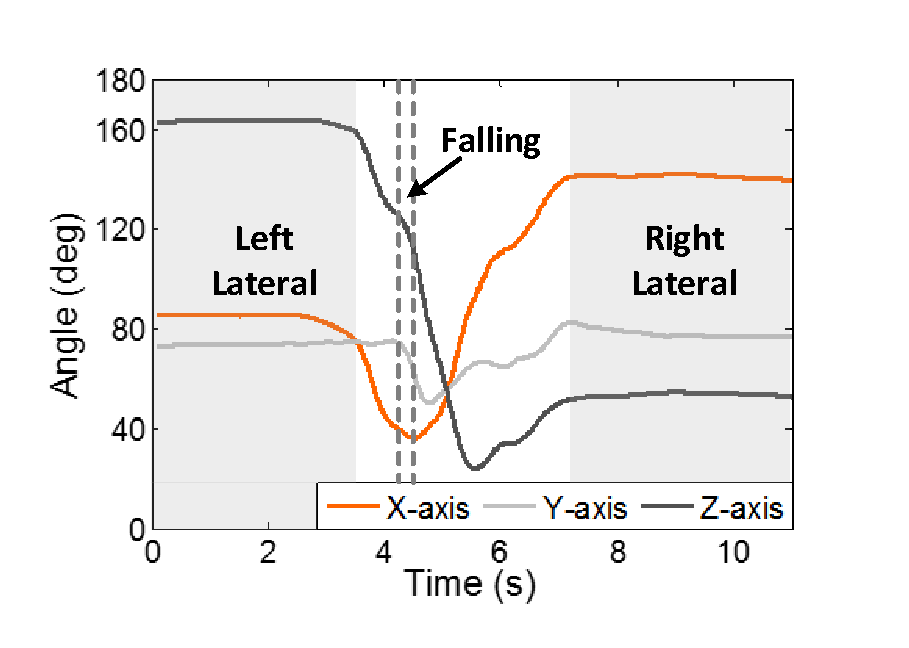
\includegraphics[width=0.97\linewidth]{Figures/LeftToRight.pdf}\centering
  \caption{From left lateral posture to right lateral posture.}\label{fig:LeftToRight}
\end{minipage}
\hspace{2pt}
\begin{minipage}[t]{0.31\linewidth}\centering
    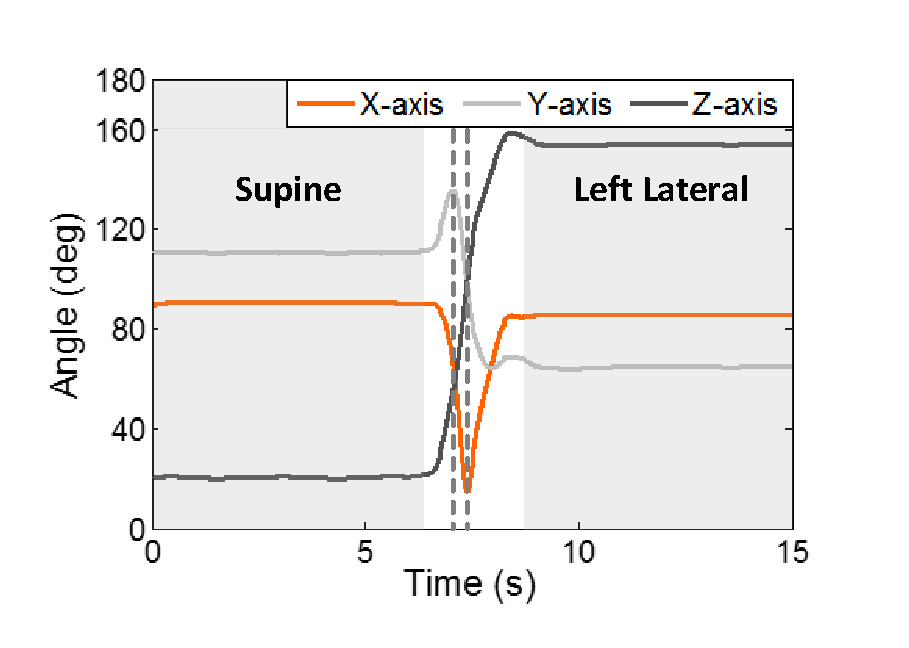
\includegraphics[width=0.97\linewidth]{Figures/SupineToLeft.pdf}\centering
  \caption{From supine posture to left lateral posture.}\label{fig:SupineToLeft}
\end{minipage}
\hspace{2pt}
\begin{minipage}[t]{0.31\linewidth}\centering
    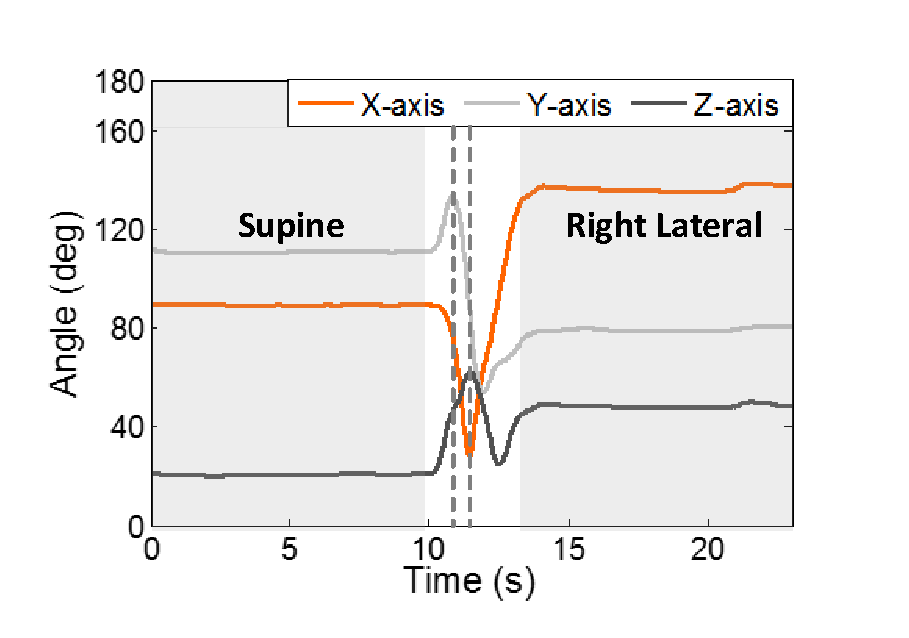
\includegraphics[width=0.97\linewidth]{Figures/SupineToRight.pdf}
  \caption{From supine posture to right lateral posture.}\label{fig:SupineToRight}
\end{minipage}
\end{figure*}

\begin{figure*}[!t]
\begin{minipage}[t]{0.31\linewidth}\centering
    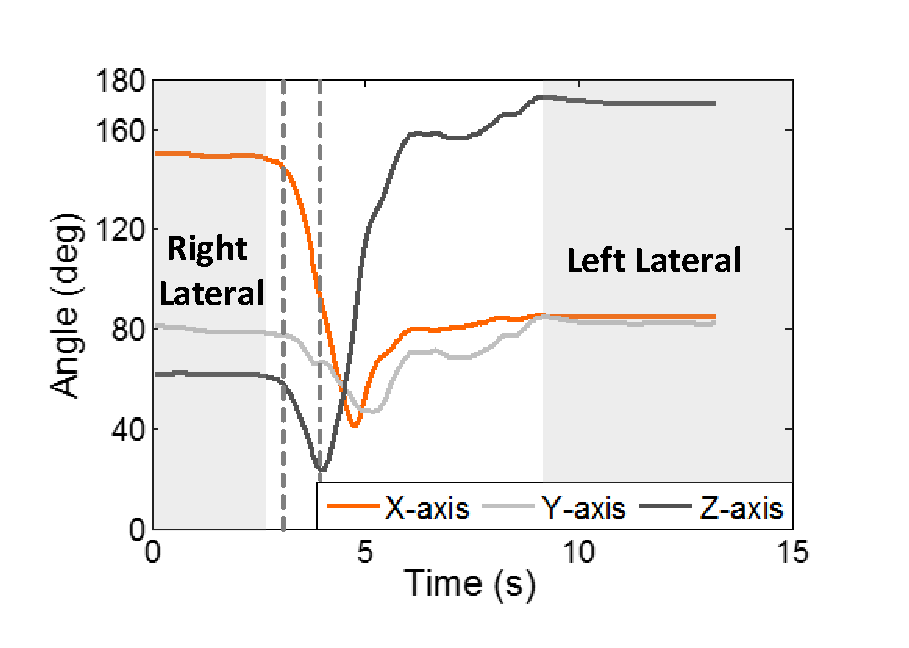
\includegraphics[width=0.97\linewidth]{Figures/RightToLeft.pdf}
  \caption{From right lateral posture to left lateral posture.}\label{fig:RightToLeft}
\end{minipage}
\hspace{2pt}
\begin{minipage}[t]{0.31\linewidth}\centering
    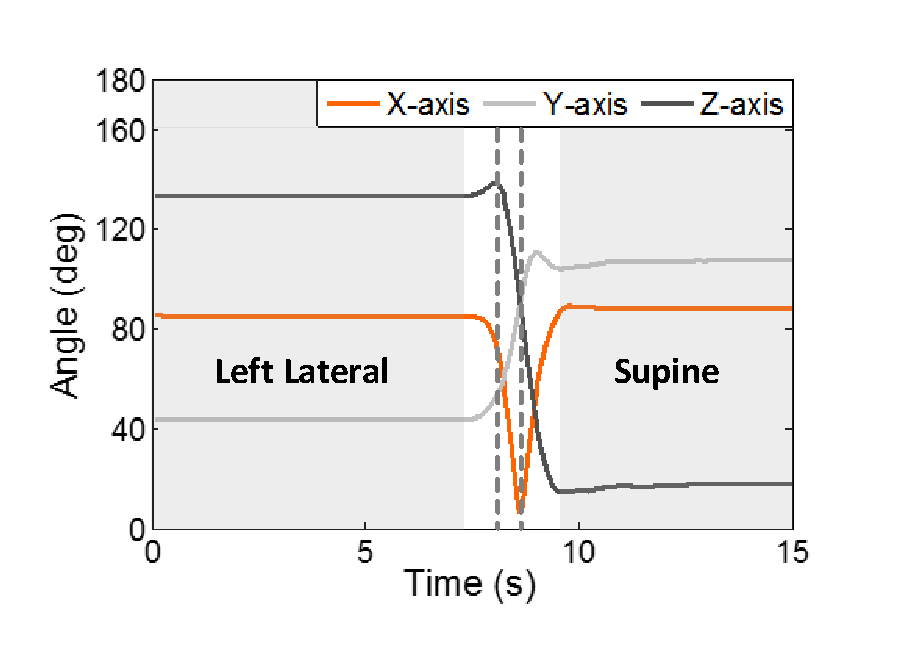
\includegraphics[width=0.97\linewidth]{Figures/LeftToSupine.pdf}
  \caption{From  left lateral posture to supine posture.}\label{fig:LeftToSupine}
\end{minipage}
\hspace{2pt}
\begin{minipage}[t]{0.31\linewidth}\centering
    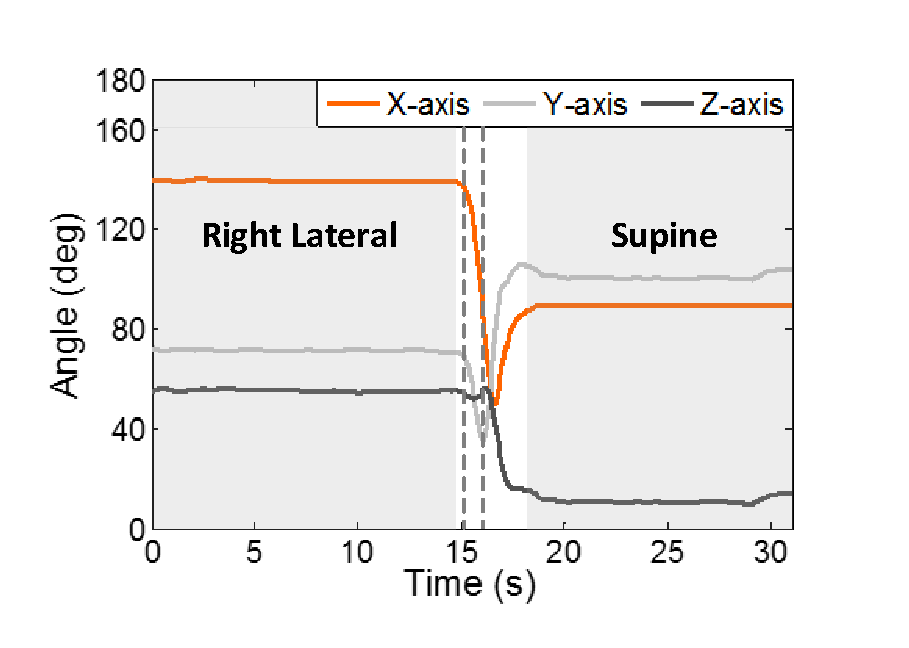
\includegraphics[width=0.97\linewidth]{Figures/RightToSupine.pdf}\centering
  \caption{From right lateral posture to supine posture.}\label{fig:RightToLeft}
\end{minipage}
\end{figure*}

To deal with this challenge, we incorporate the body postures to improve the detection accuracy. As shown in Fig. \ref{fig:BodyRollover}, the body postures are different before and after the rollover. Therefore, after we detect the time when the angle values changes, we term the time as a possible rollover time point. Then we use the sleep posture classification algorithm to determine whether the body postures are the same or not over a period of time before and after this point. \textcolor{blue}{If the postures are same, we exclude this time point, otherwise the system detects a body rollover event. In other words, a body rollover event is recorded when the posture changes
are detected between two time points.} Note that {\systemname} not only counts the number of rollovers, but also reports the exact nature of the rollover event.


\subsubsection{Micro body movement \label{sec:microbo}}

Besides major body movement, such as rollovers, there often are involuntary body movements that can affect sleep quality. With the deepening of sleep, limbs are extremely relaxed, and a little stimulus will produce trembling and micro beating. Such behavior is most likely to occur during the deep sleep stage and the REM stage~\cite{ancoli2003role,Jean2000Sleep}. Therefore, by detecting such micro body movements and distinguish them from large body movements can help us to further analyze the user's sleep stage. In this paper, we are interested in the sleep-related body movements including hand moving, arm raising, and body trembling.

The way of detecting micro movement is different from the method of detecting the body rollover as we first need to consider the influence of inherent accelerometer's noise. In addition to the appropriate data preprocessing, we need to set an appropriate threshold to classify the accelerations of micro body movements and noises. \textcolor{blue}{To set an effective threshold, we conduct extensive experiments on the 10 volunteers who participated in the training of various parameters mentioned above and ensure the accelerometer embedded in smartwatch to calculate the corresponding acceleration variance trace of the micro body movement. We use Moving Average filter with a moving window length of 35 to smooth the acceleration along the three axes,} and calculate Root Sum Square (RSS) to merge them.
\begin{equation}
      Rss(t) =\sqrt{(acc_x(t))^{2}+(acc_y(t))^{2}+(acc_z(t))^{2}},
\end{equation}
$acc_x(t)$, $acc_y(t)$ and $acc_z(t)$ represent the accelerometer sample value of x-axis, y-axis and z-axis at time stamp t respectively. \textcolor{blue}{And then we can obtain the first-order derivative of the merged acceleration.}
\begin{equation}
      V(t)=Rss(t)-Rss(t-1).
\end{equation}

Eventually, we set the threshold to be 0.03, which can achieve a satisfactory detection performance. We also observe that the micro movement duration is very short, which lasts less than 2 s. However, in our body rollover experiments, we find that the average movement duration is 3 s, as shown in Fig. \ref{fig:LeftToRight} - Fig. \ref{fig:RightToLeft}. Therefore, we can first divide the body movement events into large movement and micro movement by detecting the signal duration time. \textcolor{blue}{In order to distinguish micro-body movements, including hand movement, arm raising and body trembling, it is very intuitive to detect based on the duration of the movement, because we find that the durations of these movements are significantly different. So we try to use the duration of these movements to perform detection. However, we find that the average duration of the arm rising is 1.8 s, but the duration of the other two types of movement is around 1 s, so it is difficult to set a suitable threshold to accurately detect them. Therefore, only through the duration of the movement we can only detect the arm rising with obvious feature. For the hand movement, and body trembling is not effective. However, we have found that body  trembling is a sudden movement event, which leads to a more pronounced change in acceleration, so we can use acceleration changes to distinguish them based on such an observed fact. Specifically,  as we can see from the figure,  acceleration of body trembling has a more pronounced peak when compared to the hand movement. So we perform peak detection on the first-order derivative of the acceleration.} So we perform peak detection on the acceleration variance. For the detected peak, we calculate the difference $d$ between this peak and the average of the peaks in the reference data set. %Then for the micro body movement events including hand movement, arm raising and body trembling, we first find that the durations of these movements are significantly different. The average duration of arm rising is 1.8 s, but the duration of hand movement is only 1 s, while body tremors lasts less than 1s, as shown in Fig.~\ref{fig:micro-move}. The large difference in temporal duration makes it possible to easily distinguish raising an arm from the other types of movements. To further classify hand movement and body trembling, we observe the corresponding acceleration variance. As we can see from the figure,  acceleration of body trembling has a more pronounced peak when compared to the hand movement. So we perform peak detection on the acceleration variance. For the detected peak, we calculate the difference $d$ between this peak and the average of the peaks in the reference data set.
\begin{equation}
      d=\mid(peak-average(oi))\mid,
\end{equation}
$oi$ indicates the type of micro-movement, when $oi$ is 1, it indicates the hand movement and 2 represent body trembling.


\begin{figure}[!t]
\centering
      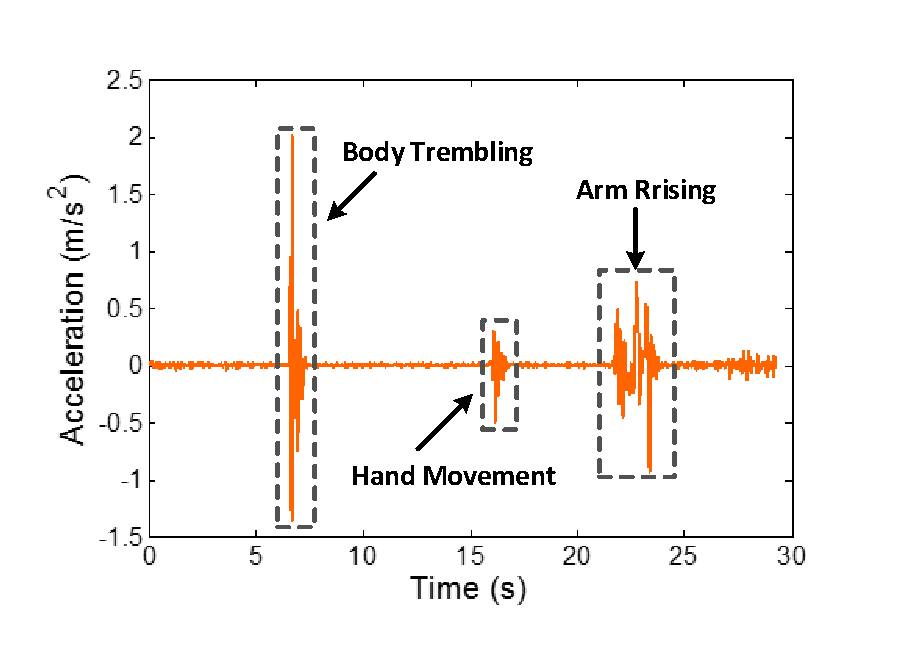
\includegraphics[width=0.43\linewidth]{Figures/Micromovement.pdf}
  \caption{Acceleration reading for micro body movements.}\label{fig:micro-move}
\end{figure}

For the two types of potential micro-movements to be classified, we calculate variances for 100 sets of micro-movement data for these 10 volunteers and perform peak detection, as well as make these peaks as features for a particular type of movement to establish a reference data set. In order to classify the micro-movement more accurately, we further obtain the average of the peak features ($average(oi)$) in the reference data set. And then we determine the type of micro-movement with the smallest value of d as the final detection result.


\subsection{Detecting Acoustic Events \label{sec:acoustic}}
Acoustic events during sleep, such as snore, cough and somniloquy, can reflect and affect user's sleep quality and physical health. For example, snore is one of the possible symptoms of cerebral infarction patients.  And long-term snoring can also have a serious impact on health and sleep. It can cause behind sleep apnea or narcolepsy, a sleeping disorder~\cite{snoring2016,snoring2013}. And when there is a cough, the human cerebral cortex cells are always in an excited state, limiting the depth of sleep, allowing only short sleep between wakefulness, like many other sleep disruptions. {\systemname} can detect these different acoustic events, including snore, cough and somniloquy.
\textcolor{blue}{Different from traditional parameters based on acoustic classification algorithm~\cite{gu2016sleep}, which is based on multi-dimensional signal feature extraction methods to detect, which will lead to high complexity of the algorithm. To avoid this problem, we directly perform physical signals detection and recognition by mining the essential characteristics of events. In other words, we exploit the inherent characteristics of different acoustic events and design a lightweight algorithm for effective classification.}%Different from traditional parameters based acoustic classification algorithm~\cite{gu2016sleep}, we exploit the inherent characteristics of different acoustic events and design a lightweight algorithm for effective classification.

\begin{figure*}[!t]
\centering
%   \setlength{\abovecaptionskip}{-2pt}
% \setlength{\belowcaptionskip}{-9pt}
%\begin{minipage}[t]{0.32\linewidth}\centering
 \subfigure[Snore of six times.]{\label{snore}
   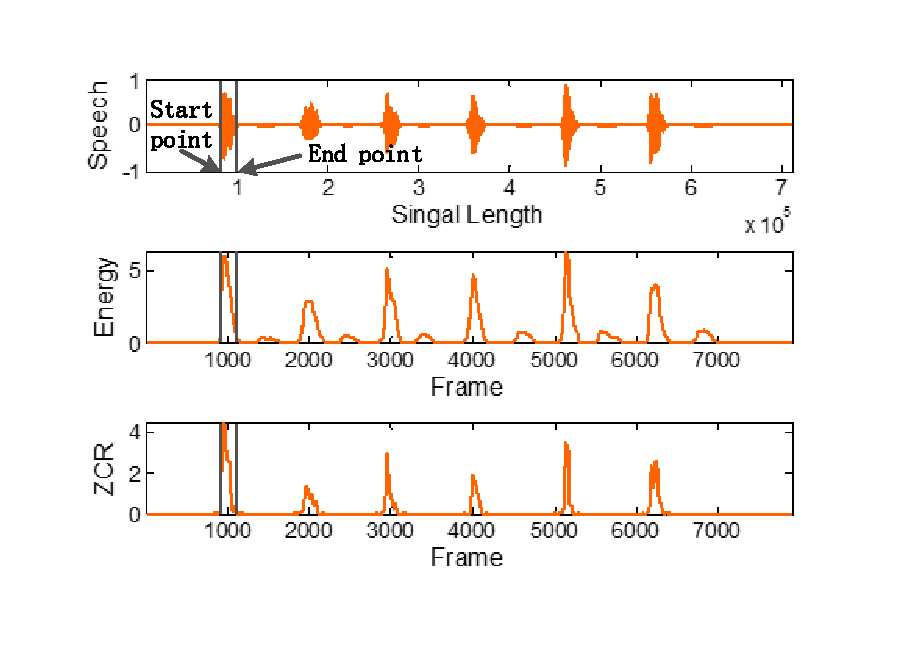
\includegraphics[width=0.32\linewidth]{Figures/snore.pdf}}
 \subfigure[Two consecutive cough.]{\label{cough}
   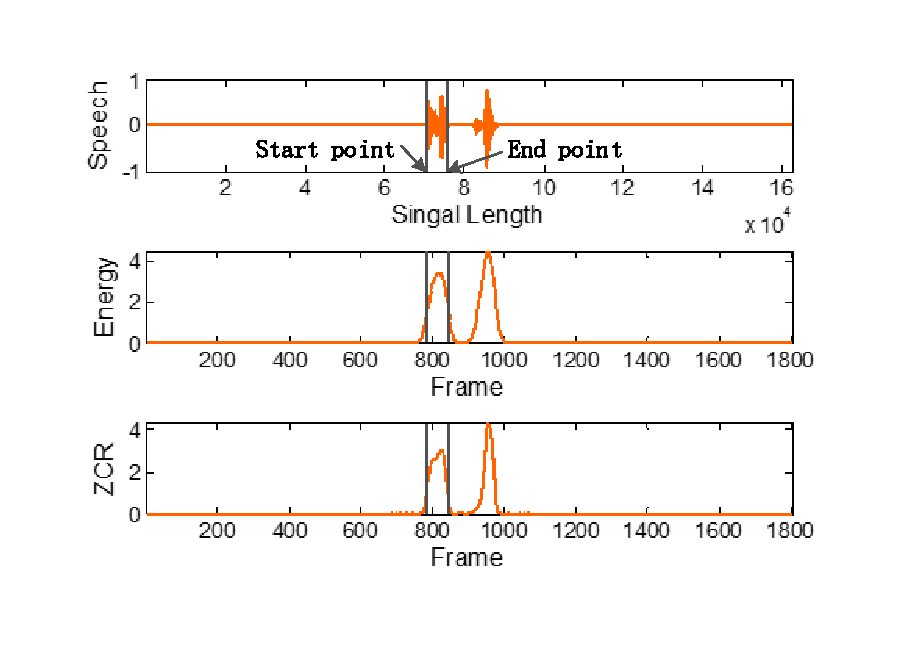
\includegraphics[width=0.32\linewidth]{Figures/cough.pdf}}
\subfigure[Somniloquy.]{\label{somniloquy}
     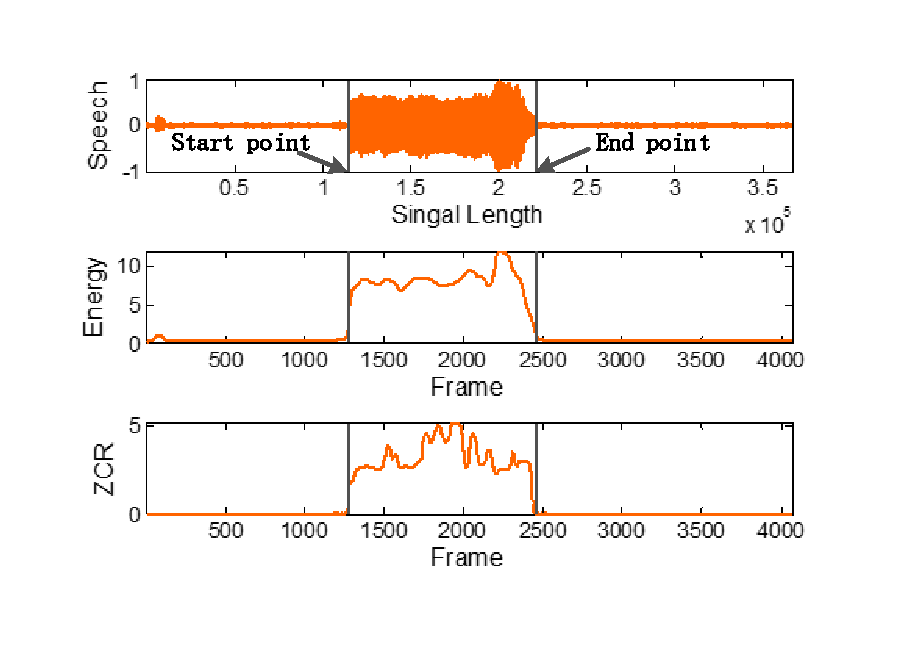
\includegraphics[width=0.32\linewidth]{Figures/somniloquy.pdf}}
\caption{The characteristics of different acoustic events.}\label{acoustic}
\end{figure*}


\subsubsection*{Acoustic feature calculation}
In order to identify different acoustic events accurately, we select the short-term average energy and the zero-crossing rate as two features. The short-term average energy of acoustic signal is computed as:
\begin{equation}
  E_i=\sum\nolimits_{j=-\infty}^{\infty}[x(j)\omega(i-j)]^2=\sum\nolimits_{j=i-(N-1)}^{i}[x(j)\omega(i-j)]^2,
\end{equation}
$N$ is the window length, $x$ is the signal and $\omega$ is the impulse response. As we can see that the short-term energy is the weighted
sum of squared frame sample. The short-term energy can be used to distinguish the segment of unvoiced and voiced sound. It also can be used
to differentiate speech segment and noise segment  in  case of relatively high signal to noise ratio (SNR). The zero-crossing rate is
computed as:
\begin{equation}
  Z_i = \frac{1}{2}\sum\nolimits_{j=0}^{N}|sgn[x_i(j)]-sgn[x_i(j-1)]|.
\end{equation}
It indicates the number of times, which the acoustic signal waveform passes through the horizontal axis (zero level). We carry out an interesting recognition experiment using the microphone built in smartwatch to detect the sound of people during sleep and effectively identify different acoustic events. We focus on three common acoustic events: snore, cough and somniloquy. Ten volunteers worn the smartwatches during sleep to record the acoustic data. We manually label the data with different acoustic events. Fig. \ref{acoustic} shows the acoustic characteristics of  three events. There are six times snore event, two consecutive cough event and somniloquy event.
%The sample rate is 22050 Hz.


\subsubsection*{Acoustic event recognition}
 At beginning, the algorithm  divides the audio stream into frames with equal durations. Each frame is composed of 256 samples, and its duration is 12 ms. To identify the  three common acoustic events, we introduce an acoustic recognition algorithm based on the following key observations:

 \begin{itemize}[itemsep=1mm,nolistsep]
\item The time interval between two signals for different acoustic events are quite different from each other. As shown in Fig.~\ref{snore}, there is a long time interval between two snores. While, the time interval between two coughs is very short.  In contrast, the  somniloquy signal is irregular and without periodic property.
    %Besides, the snore event produces periodic signals and their intervals  are similar.
 \item The duration of one signal for different acoustic events are different from each other. Fig. \ref{acoustic} shows that the duration of a snore is shorter than the duration of a cough and somniloquy. And in general, the duration of a cough is shorter than the duration of a somniloquy signal.
\item The frequencies for different acoustic events are quite different from each other. Snore event has a continuous signal, while the  cough and somniloquy are sudden events, thus the number of consecutive occurrences is very small.
\end{itemize}
In conclusion, the ``interval'', ``duration'' and ``frequency'' of acoustic events can be used as three unique features. Based on the above three observations, our acoustic event recognition algorithm involves the following two steps. First, in order to estimate the interval and frequency of an acoustic event, we perform the peak detection. We use the short-term average energy to calculate the peak value of the acoustic signal. When the peak exceeds a certain threshold, such as 3 dB in this paper, we record the position of each peak and calculate the interval between two consecutive peaks. Next, we can estimate the frequency of an acoustic event by counting the number of peaks over a time window. Second, to estimate the duration of the acoustic event, we perform the start-point and end-point detection.

Traditional end-point detection algorithm \cite{stowell2015detection}, however, uses a fixed double threshold and must be obtained by a large number of data samples, which has two drawbacks. First, the fixed double threshold may cause error detection at the beginning of acoustic event. Second, the requirement of a large number of data samples would lead to large system latency. \textcolor{blue}{To deal with those problems, we introduce an improved end-point detection method, which does not require pre-sampling learning to obtain the threshold parameters. Instead, it utilizes the information of each signal to be detected to perform threshold estimation, which not only reduces the number of data samples and the costs of learning but also leads to higher detection accuracy.} The proposed method has a adaptive threshold, in detail, Since the first few frames and the last few frames are mostly mute or background noise, we select the first five frames and the last five frames to calculate their short-term energy, which are denoted as $E_s$ and $E_e$, respectively. And then the two are combined to obtain the mean $E_n$ as the estimated energy value of the noise segment.Let the maximum value of the short-term energy over all frames denoted as $\max (E)$. Then, the average short-term energy $DE$ is given as:
\begin{eqnarray}
      &E_n = \frac{(E_s+E_e)}{2}, \\
      &DE = \max (E)-E_n.\label{eq:DE}
\end{eqnarray}

So we can use $EH$ and $EL$ to represent the high and low threshold of short-term energy, which are given as:
\begin{equation}
      EH=\alpha \times DE+E_n,
\end{equation}
\begin{equation}
    EL=\beta \times DE+E_n,
\end{equation}

 \textcolor{blue}{$\alpha$ and $\beta$ are the multiplier factor of the energy value DE. In order to set the energy threshold for detecting the start and end points of the speech signal, we first need to consider that this threshold must be greater than the energy of the noise signal ($E_n$) to ensure that the noise is filtered out. And then we need to get select the appropriate $\alpha$ and $\beta$ to ensure that we get the proper double threshold to accurately detect the start and end points. Specifically, we used the nighttime sound data of 10 volunteers who participated in training to train the multiplier factor of the energy value DE of the speech signal throughout the frame. We vary $\alpha$ from 0.1 to 0.5 and $\beta$ from 0.01 to 0.09, eventually set $\alpha$ to be 0.1 and $\beta$ to be 0.06, which achieves the best detection performance.}

 Moreover, in order to avoid the interference of sudden noise, we set the minimum length of the signal segment and count the length of the signal during the search for the start and end point. Finally, if the signal length is less than the set minimum, it is considered as a noise segment. The results of the start-point and end-point detection are shown in Fig. \ref{acoustic}, we calculate the length of each speech segment and calculate their averages as the duration of the acoustic event. Last, we count the number of peak points to determine whether it meets the third key observation or not.



%Algorithm 1 provides the detailed  process of the start-point  and end-point detections.


%$A_x$, $A_y$ and $A_z$ are the tilt angle of the three axes, and $\omega_x$, $\omega_y$ and $\omega_z$ are the rotation speed of the three axes. So $\phi$, $\theta$ and $\psi$ are the rotation angle of the three axes. \textcolor[rgb]{1.00,0.00,0.00}{(Those symbols do not present in Algorithm 1)}


%\begin{table}[!thbp]
%\begin{tabular}{l}
%  \hline
%  \textbf{Algorithm 1} The Endpoint Detection \\
%  \hline
%  \textbf{Input}: A sound signal recorded by the microphone:$x$
%  \\\quad \quad \quad The threshold of zero-crossing rate:$ZT$
%  \\\quad \quad \quad The minimum length of speech:$minlen$\\
%  \textbf{Output}:The start-point  and end-point :$p_s,p_e$\\
%  1: Split  $x$ using the framing algorithm \\
%  2: Calculate each frame of energy and zero-crossing rate:$E_i,Z_i$ \\
%  3: Calculate the threshold for short-time energy:$EH,EL$  \\
%  4:$count=0$,$silence=0$\\
%  \textbf{the start point}\\
%  5:\textbf{for}i=1$\rightarrow \frac{length(x)}{frame~length}$  do\\
%  6: \textbf{if} $ E_i>EH $ \textbf{then}\\
%  7: $count=count+1$,$silence = 0$,$max(n-count-1,1)=p_s$\\
%  8: \textbf{else if} $E_i>El || z_i>ZT $\textbf{then}\\
%  9: $count=count+1$ \\
%  10: \textbf{else}\\
%  11:$count=0 $ \\
%  12: \textbf{end if}\\
%  \textbf{the end point}\\
%  13:\textbf{if} $E_i>El || z_i>ZT $\textbf{then}\\
%  14:$count=count+1$ \\
%  15:\textbf{else}\\
%  16:$silence = silence+1 $ \\
%  17:\textbf{if} $count < minlen$\textbf{then}\\
%  18:$count=0 $, $silence=0$ \\
%  19:\textbf{end if}\\
%  20:$count1 = count-\frac{silence}{2}$\\
%  21:$ p_e = p_s + count1 -1$ \\
%  \hline
%\end{tabular}
%\end{table}


\subsection{Tracking Illumination Conditions \label{sec:illumination}}
Studies have shown that there is a significant interaction between illuminance level and the mental state of the individual \cite{light77}.
For example, the bright light can counteract subjective fatigue during daytime, but at night it will seriously affecting the sleep quality.
Too much light exposure can shift our biological clock, which makes restful sleep difficult to achieve, it affects our sleep and wake cycle
\cite{light2007}.  Besides, we also note that the dim light will affect our sleep too. According to the study \cite{light2016}, it can be
learned that the dim artificial light during sleep is significantly associated with the general increase in fatigue, and the proper light
can be used to increase the sense of exhaustion and promote sleep. So illumination condition in a sleeping environment has a significant
influence on sleep. {\systemname} use the ambient light sensor to detect the illumination condition during sleep. We visit 10 volunteers'
bedroom at night and the use of the ambient light sensor to test the lighting conditions in the bedroom, \textcolor{blue}{and we find that
in the absence of light in the bedroom, the reading of the light sensor is basically maintained at 1Lux to 4Lux. In some cases, the watch's
screen is awakened and lighted up to cause the light to rise to 4Lux; when the bedroom is in a faint light, such as a table lamp light, the
light sensor's average readings are also maintained below 10Lux. So ultimately we will divide the illumination intensity into two
conditions: bedroom without light (Weak illumination condition, $\leq$ 10Lux);  bedroom with strong lights (Strong illumination condition,
$>$ 10Lux).} Therefore, we can learn the light conditions in the sleeping environment according to the two types of illumination
conditions.

However, the light sensor may be obscured, which leads to large errors in measuring the illumination level. For example, a user's smartwatch may be covered under quilt when he/she turned over unconsciously, and thus the illumination readings on the smartwatch may not reflect the real lighting situation. \textcolor{blue}{Previous work has used the smartphone to detect the illumination conditions and also encountered the situation where the light sensor was blocked. To deal with this problem, they chose to introduce another sensor in the smartphone, the proximity sensor,  to detect whether the light sensor is blocked or not. However, it does not apply in smartwatch because there is no proximity sensor.} To deal with this practical challenge, the key is that the illumination would drop suddenly when the smartwatch is covered by other objects. There are two possibilities for the sudden drop in light intensity. For most smartwatches, the light sensors are usually installed in the front face of it. The first case is the indoor lighting facilities are closed. The second case is the wrist turned so that the back of the hand become downward, thus blocking the light sensor in front of the smartwatch. \textcolor{blue}{In fact, this situation can easily occur. For example, when a user change sleeping posture to the left side, the user's hand may be close to the pillow with the palm facing up. Or there is a micro body movement like the hand movement so that the back of the hand become downward.} To avoid this erroneous illumination condition measurement, we detect whether the user is performing a wrist flip over a period of time during the intensity plummeting. We detect the wrist flip based on two aspects: (i) the rotation angle of smartwatch; (ii) whether the light intensity maintains stable after the sharp drop. If the wrist flips, we use the average of the previous light intensity as the intensity of the time period. It should be noted that, because the illumination condition detection algorithm is relatively simple, it is not explained in the experimental part.

\subsection{Sleep stage and quality}
\textcolor{blue}{Physiological communities often regard sleep as a cyclical process composed of three stages: rapid eye movement (REM) stage, light sleep stage and deep sleep stage. REM is an active period of sleep marked by intense brain activities and dream occurrence. Light sleep stage is a period of relaxation, when the heartbeat, breathing rate and muscle activity slow down. Deep sleep stage triggers hormones to promote body growth, as well as the repair and restoration of energy.  The biological characteristics of different sleep stages exhibit distinguishingly. In clinical sleep study, the sleep stages are mainly identified by simultaneously evaluating three fundamental measurement modalities including brain activities, eye movements, and muscle contractions. The EEG measure using electrodes placed around the scalp interpret various sleep/wake states of the brain. And, EMG and EOG using electrodes placed on the skin near the eyes and on the muscles, respectively, measures in deeply differentiating REM stage from all the other stages. But, apart from the implicit physiological activities, sleepers usually exhibit distinguishable physical activities in different sleep stages. For example, there are somniloquy and body trembles caused by frequent dreams generally appear in REM, large body movements such as body rollovers and arm raising happen in light sleep and micro body movements such as body trembling and snoring occur in deep sleep.  In the meanwhile, the breathing amplitude in NREM stage is larger compared with the REM stage. Moreover, sleep cycle usually repeats four to six times over a night. The sleeper usually experiences a transition from light sleep to deep sleep and then enters REM, but sometimes there is also possible a phenomenon of skipping some certain sleep stages occurs during sleep. However, despite this, dependence between two successive sleep stages still exists and different sleep stages have potential conversion probabilities, which also mentioned in Sleep Hunter \cite{gu2016sleep}. }

\textcolor{blue}{Thus, based on these features, we build a Hidden Markov Model \cite{johnson2010hidden}. And we use a series of sleep events as the observed sequence and the sleep stage as the implicit stage sequence. $obs_t={NB(t),NB_M(t),BA(t),NA(t)}$ represents the feature vector at detection phase t. The explanation of each item, which is the input of HMM, is listed as follows. $NB(t)$: the number of occurrences of body rollover during the detection phase t. $NB_M(t)$: the number of occurrences of micro body movement. $BA(t)$: the measurement of  respiratory amplitude. $NA(t)$:the number of occurrences acoustic events. And $states_t$ =$\{$light sleep; deep sleep; REM$\}$ is an output of our model, which represents the sleep stage in the detection phase t. In the training of the HMM model, we used nocturnal sleep data from 10 volunteers who participated in the training parameters of each algorithm and make their sleep-related events as observation sequences and the corresponding sleep stages detected by Fitbit as hidden state sequences, to generate HMM models. Specifically, we first use maximum likelihood estimation method for parameter estimation, the state transition matrix and the confusion matrix, and then use the Viterbi algorithm [38] to acquire a series of implicit state sequences corresponding to observed sequence.} As a result, we can estimate the sleep stage during a time window. Finally, we can get the durations of all sleep stages over the whole sleep process.

Further, to quantize the quality of a sleep, we use the Sleep Quality Report model introduced in \cite{gu2016sleep}. Let $SQ$ be the value of the sleep quality, then $SQ$ is given as follow:
 \begin{equation}
SQ=\frac{(REM \times 0.5+Light \times 0.75+Deep) \times 100}{REM+Light+Deep}
 \end{equation}
where, REM, Deep and Light represents the duration time in a sleep process. The range of $SQ$ is from 50 to 100. A high value of $SQ$ shows a good  sleep quality.

\section{Evaluation Methodology}
\label{sec:expsetup}

\subsection{Implementation \label{sec:implementation}}
We prototype and evaluate \systemname on a Huawei Smartwatch 2 wearable device. The smartwatch is equipped with a Quad-core Cortex-A7
processor at 1.1 GHz.  It runs the Android Wear 2.0 operating system. We use five sensors of the smartwatch: the accelerometer, gyroscope,
microphone, light sensor and orientation sensor. To reduce energy consumption of the smartwatch, in our experiments we analyse the sensor data on a a XiaoMI Note2 Android smartphone to which the smartwach sends sensor measurements over Bluetooth, \textcolor{blue}{and the data is collected every 30 ms on the smartwatch. Although our sampling rate is not very high, it is sufficient for detecting the sleep-related events and this can save energy consumption of the watch compared to a high sampling rate.} %The collected sensor data are sent via Bluetooth to a XiaoMI Note2 Android smartphone for post-processing and
%event detection.

\systemname starts tracking sleep events when it detects that the light is off and there has been no body movement for 30 minutes. As part of an initialization process, \systemname estimates the initial body posture and hand position. It then uses these as a starting point to monitor sleep events like the body posture, rollovers, hand positions and body movements.

\textcolor{blue}{And in order to improve the effectiveness of {\systemname} in detecting sleep posture, we need to consider as many arm positions as possible in different sleep postures, and ensure that the positions we choose are suitable for most people. So we randomly selected 100 volunteers. The ages ranged from 16 to 60 years old, and questionnaires were used to discuss their sleep posture during their daily. The main content of the questionnaire was about their common arm position in 4 different sleeping postures. Based on this investigation and some study of previous related works\cite{position2014,HandPosition2}, we finally selected those positions to be our the basis for the study of sleep position detection. And we also found that the positions of these arms are effective during the training and testing of the algorithm.}



\begin{figure}[!t]
	\centering
	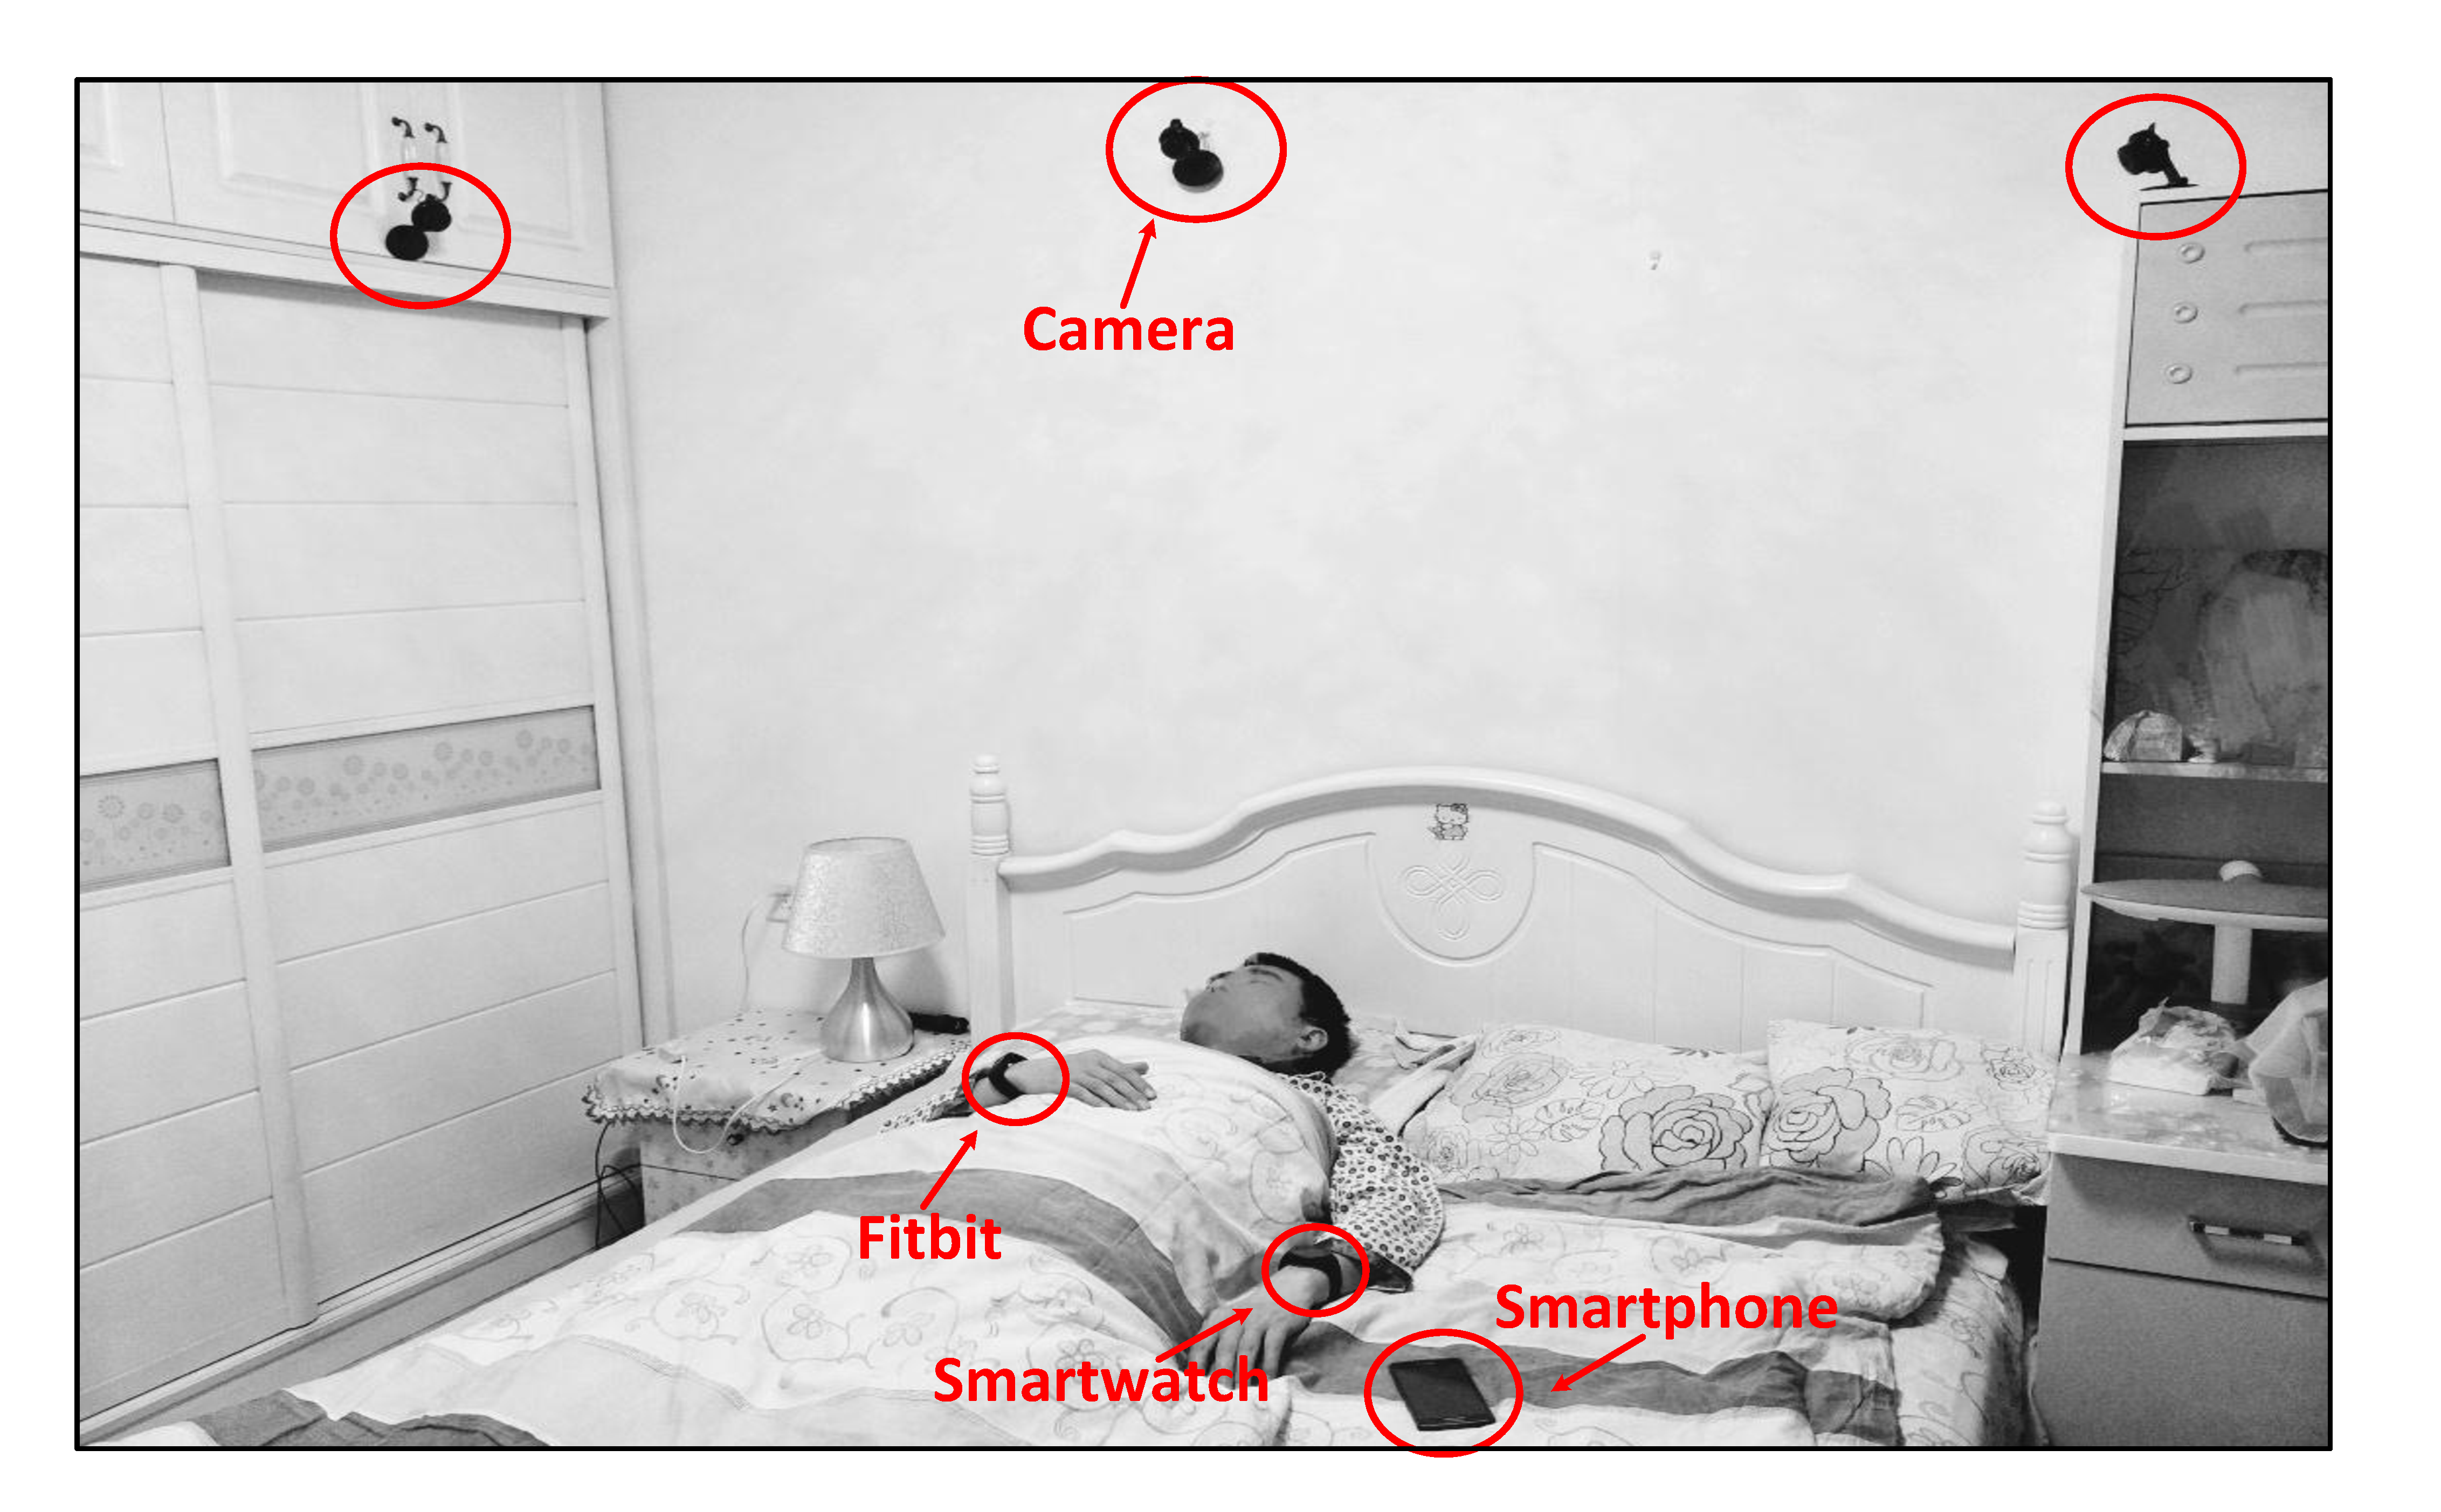
\includegraphics[width=0.75\linewidth]{Figures/setup.pdf}
	\caption{Experimental setup in one of our participants' home. }\label{fig:setup}
\end{figure}



%\section{Experimental Setup} {\systemname} is implemented on the HuaWei Smartwatch 2. The programming platform is JAVA. For simplification,
%we implement the event detection on a laptop and the collected data is processed by MATLAB. \textcolor{blue}{In our experiments, we recruit
%15 volunteers (6 males and 9 females) from 15 years old to 60 years old,  of whom 5 people are between the ages of 15 and 25, and 5 are
%between the ages of 25 and 40, and 6 people between 40 and 60 years old. According to our preliminary survey of participants, two of 40 to
%60 year old are found to have long-term sleep disorders,  one with difficulty falling asleep and having a light sleep with more dreams, and
%another participant with the symptoms of awaking at night and early awakening, and there is a 53-year-old participant have been troubled by
%snoring, they are the focus of our attention. In addition, other participants occasionally suffer some sleep problems such as insomnia,
%snore and so on.} The experiments are conducted over two weeks, and during experiments, these volunteers sleep alone in a quiet room and
%each of them sleeps at least 6 hours. Moreover, each participant is asked to wear a smartwatch and Fitbit Charge2 \cite{fitbit} on his/her
%wrist simultaneously during sleep. And the smartphone with Sleep As Android \cite{SleepAndroid} is placed beside the participant's body.
%Considering that there is no absolute ground truth to detect sleep stage and the operations of other professional medical equipment are
%complicated, we leverage the result of Fitbit Charge2, a comfortable and effortless bracelet, as the ground truth. Sleep As Android, a
%widely used app for sleep detection, run the whole sleep process for comparing with our system. At the same time, to test the reliability
%of our methods, we use the video camera to monitor the sleep, and those recorded data by camera are set as groundtruth during the
%experiment. \textcolor{red}{Fig.00000} illustrates the experimental scene for our system.



\subsection{User Participation} We have recruited 15 volunteers to participate in our experiments. Our
participants include 6 males and 9 females, whose age spans 15 to 60 years. \textcolor{blue}{And the 15 participants are different from the 10 participants who participated in the parametric training.} Two of our participants have been diagnosed with long-term,
on-going sleep-related disorders, and one participant has described that his sleep is significantly affected by snoring. The rest of our
participants report their sleep quality as up and down and they could have poor sleeps from time to time.

\subsection{Experimental Setup}
After obtaining IRB approval and consents of our participants, we have conducted our experiments at 15 homes over a two-week period. We
collected 210 sets of nocturnal sleep data from our participants. During the experiment, our volunteers slept alone in a bedroom at
home, and they slept for at least 6 hours per day.


Our participants are asked to wear a smartwatch on their wrists. Fig.~\ref{fig:setup} shows the experimental setup where we placed three
video cameras on the ceiling to monitor the user's sleep activities. The cameras have night vision and thus can record high-quality videos
at nights. We inspect the video footage to manually label the user's sleep activities and use these as the ground truth to evaluate \systemname. \textcolor{blue}{We use the sleep stages reported by Fitbit Charge2 which is proven to have a good association of movement measurements and to be comparable to PSG in adults ~\cite{evenson2015systematic,fitbit01,fitbit02,fitbit03}, especially in estimating REM and light sleep stage. As we know, Fitbit is a commercial state-of-the-art and a popular sleep monitoring wristband. It has less interference with the subject's normal sleep process, making easier for subjects to relax and maintain normal sleep. However, even if PSG has high accuracy in monitoring sleep, it may have some impact on their psychological and normal sleep processes (as it requires the user to wear many instruments) , so as not to reflect the actual sleep conditions. Moreover, Fitbit is inexpensive and easy to deploy, so it is very convenient to apply to our large number of home-style experimental scenarios.} Therefore, our participants are asked to wear two smartwatches on their wrists: a Fitbit Charge2 that runs the Fitbit app and a Huawei Smartwatch 2 that runs \systemname.

We compare our approach against Sleep Hunter~\cite{gu2016sleep}, a state-of-the-art mobile-based sleep monitoring approach, and a
smartphone-based sleep monitoring app named Sleep as Android~\cite{SleepAndroid}. To provide a fair comparison, we also place a smartphone
next to the user's body on the bed to collect the data for Sleep Hunter and Sleep as Android.

\section{RESULTS}\label{sec:4experiment}
In this section, we detail the evaluation results for our system.

\subsection{Evaluation of Subcomponents}
We focus on the detection accuracy about five events, that are body posture, the body rollover, the hand position, the micro body movement and the acoustic events.
%, the classification of micro body movement

\subsubsection{Sleep Posture Classification Performance}
\label{subsub:bodyposture}

We test the overall classification performance of different body postures. The groundtruth of body postures are recorded by the cameras. \textcolor{blue}{We use a modified cross-validation approach, which is different from the traditional leave-one-out cross-validation approach. We train the classifier by using only a single user's data, and tested the rest fourteen users.} The motivation for using data from a single user as training data is to highlight the capability of \systemname to accurately characterize body posture with very little training data, while at the same time being able to generalize across users. \textcolor{blue}{Using our method can not only achieve the purpose of cross-validation, that is, the results are more fair and reliable, but also get results in a shorter time, reduce the time cost.} The final performance is then calculated as the averaged accuracy across the 15 folds; as shown in Fig.~\ref{fig:posture_zhu}. We can observe that the posture detection accuracy is consistently high across all users, and does not show major variations across users. This good performance benefits from the distinct characteristics of arm position under different sleeping postures. Compared to results reported for SleepMonitor~\cite{sleepmonitor}, \systemname consistently improves performance which is mainly due to the template-based classifier that we use to verify classifications of the prone and supine states. In particular, \systemname achieves around $5$ percentage units higher performance on the prone state than SleepMonitor and overall has a lower false positive rate.

\begin{figure}
	\centering
	\begin{minipage}{.5\textwidth}
	 \centering
	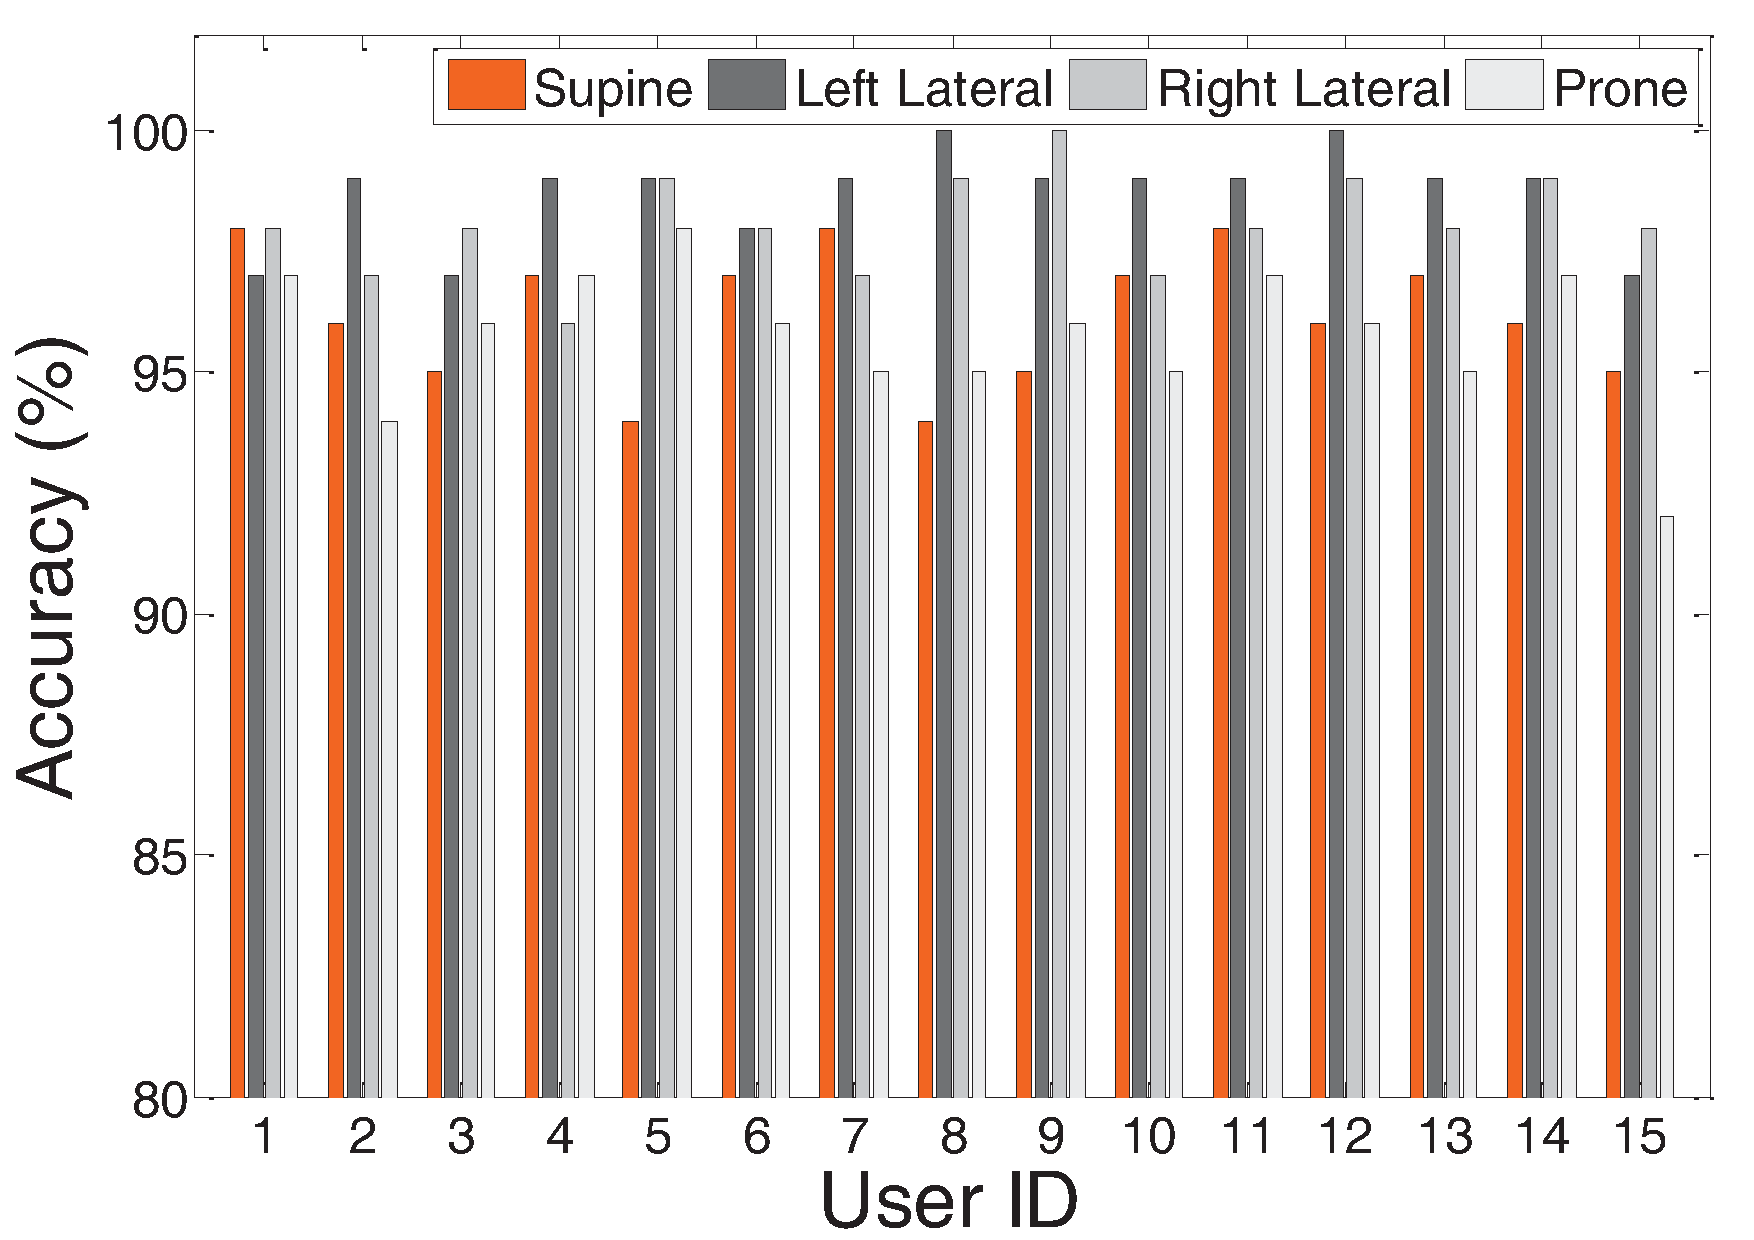
\includegraphics[width=0.95\linewidth]{Figures/posture_zhu.pdf}
	\caption{Detection accuracy of body postures.}\label{fig:posture_zhu}
	\end{minipage}%
	\begin{minipage}{.5\textwidth}
			\centering
		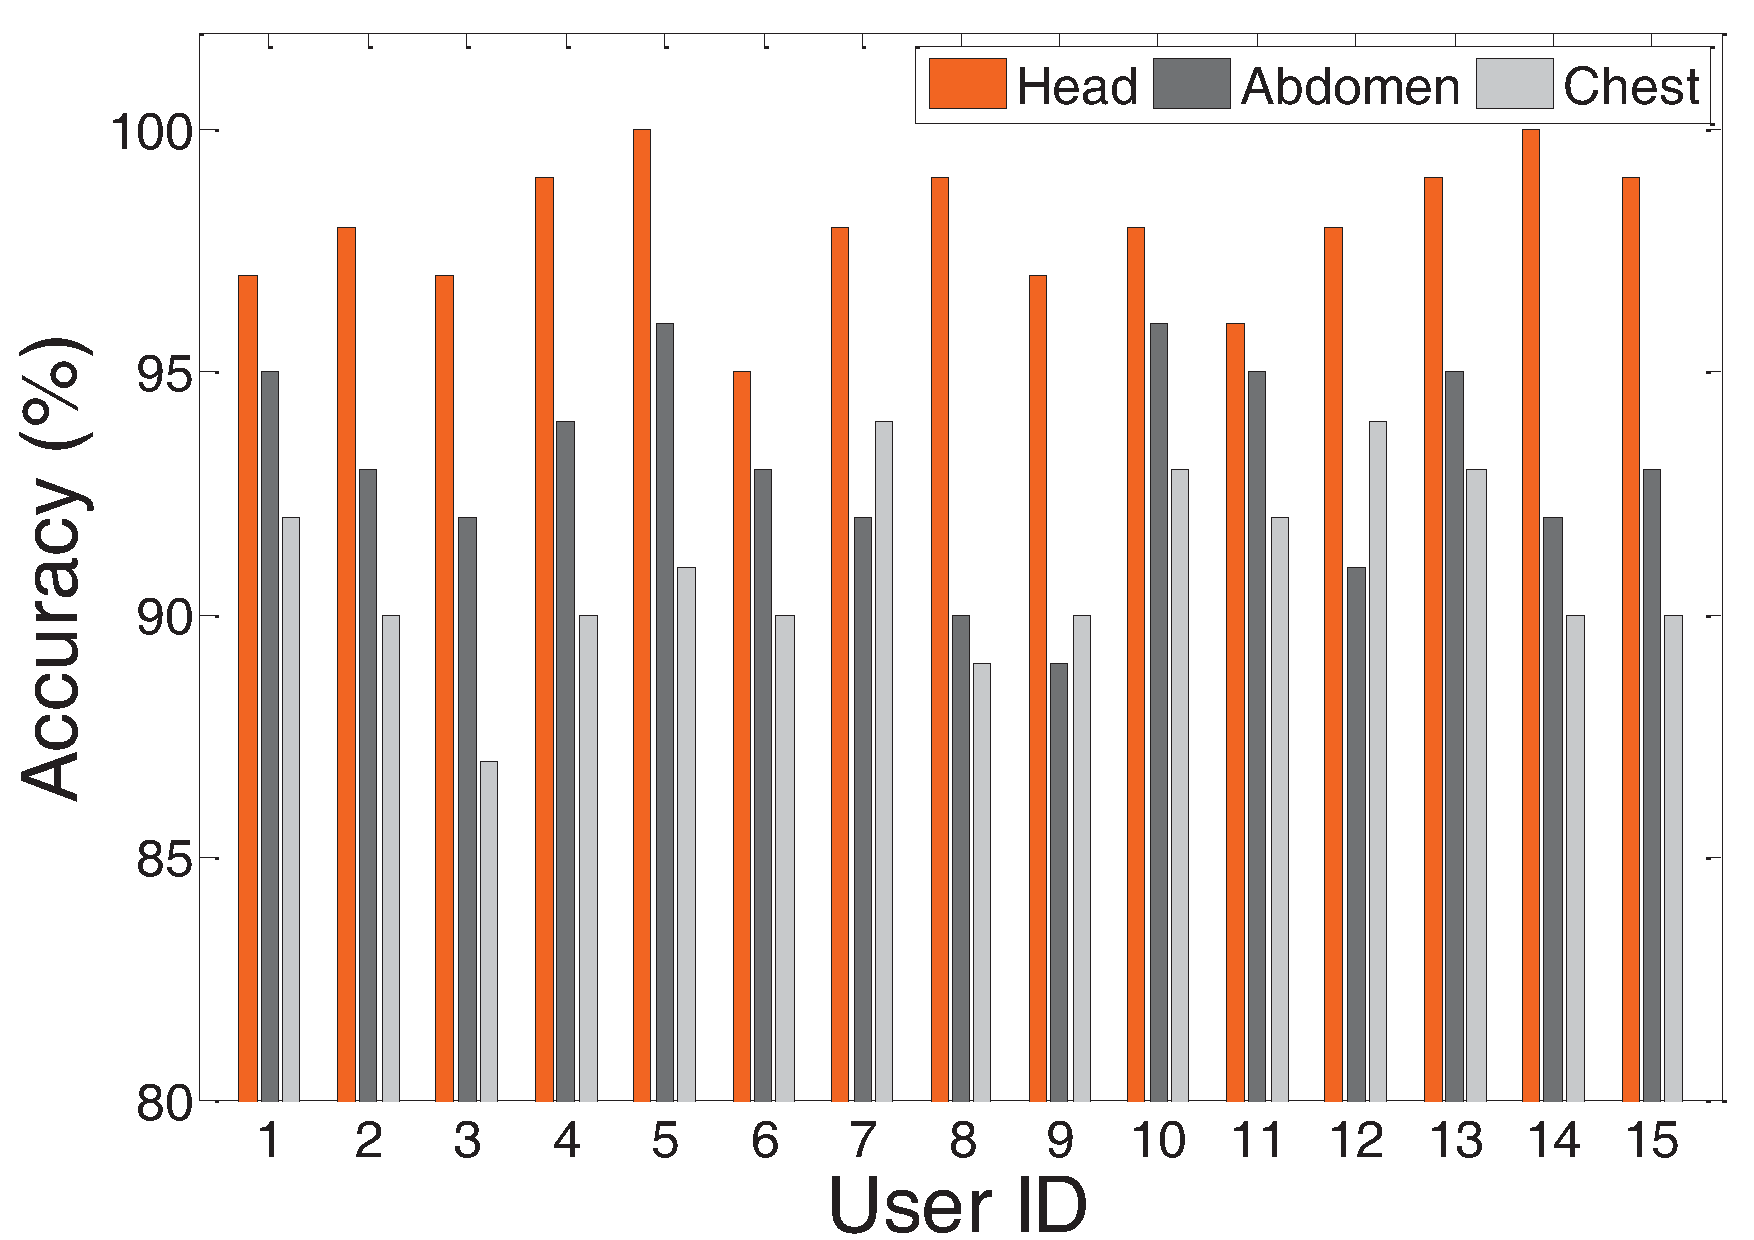
\includegraphics[width=0.95\linewidth]{Figures/handposition_zhu.pdf}
		\caption{Identification accuracy of hand positions.}\label{fig:hand_zhu}
	\end{minipage}
\end{figure}

\begin{table}[!thbp]\footnotesize
%	\tabcolsep1pt
	\centering  % ������
	%\renewcommand\arraystretch{0.277}
	%\caption{The confusion matrix of body posture classification.}\label{tab:posture}
	%\noindent\makebox{%
	%\begin{tabular}{1\textwidth}{ c | c | c | c | c | c | c}
	\renewcommand\arraystretch{0.3}
	\caption{The confusion matrix of body posture classification.}\label{tab:posture}
	\begin{tabular}{c| c | c | c | c | c | c}
		\cline{1-7}
		&\multicolumn{1}{ c|}{ }
		& \multicolumn{4}{ c|}{ }\\
		\multirow{2}*{}
		&\multicolumn{1}{c|}{\multirow{2}*{{Result}}}
		&\multicolumn{4}{c|}{{Prediction}}
		& \multirow{4}*{{Recall}} \\
		%&\multicolumn{5}{ c |}{\textbf{\small Prediction}} \\
		% & \multicolumn{5}{ c |}{ } \\
		\cline{3-6}
		& & & & & \\
		\multicolumn{1}{c|}{{}}
		&  \multicolumn{1}{c|}{{}}
		&  \multicolumn{1}{c|}{{Supine}}
		&  \multicolumn{1}{c|}{{Left Lateral}}
		&  \multicolumn{1}{c|}{{Right Lateral}}
		&  \multicolumn{1}{c|}{{Prone}}   \\
		& & & & & \\
		\cline{1-7}
		& & & & & \\
		\multirow{5}{*}{\begin{sideways}{{Groundtruth}}\end{sideways}}
		&   {Supine}   & {\bf{{1182}}}    &   $25$      &   $4$      &   $9$    &   {96.7\%}\\
		& & & & & \\
		\cline{2-7}
		& & & & & \\
		&   {Left Lateral}   &   $6$      &   {\bf{{1292}}}     &   $0$      &   $0$   &   {99.5\%} \\
		& & & & & \\
		\cline{2-7}
		& & & & & \\
		&   {Right Lateral}   &   $7$      &   $0$      &  {\bf{{1275}}}      &   $12$  &   {98.5\%}  \\
		& & & & & \\
		\cline{2-7}
		& & & & & \\
		&   {Prone}   &   $19$      &   $2$      &   $3$      &   {\bf{{567}}}   &   {95.9\%} \\
		& & & & & \\
		\cline{1-7}
		& & & & & \\
		&   {Precision}    &   {97.3 \%}   &   {98.0\%}   &   {99.5\%}   &   {96.4\%}    \\
		& & & & & \\
		\cline{1-7}
	\end{tabular}
\end{table}

To have a deep evaluation about the sleep posture detection, we randomly choose one user to train the classifier. Then we calculate the detection precision and recall across postures. \textcolor{blue}{The averaged results across our 15 participants is shown in Table \ref{tab:posture}.} The values in blocks are the corresponding numbers of four sleep postures from 14 test users. Due to that the angle features of acceleration are similar between the supine posture with hand putting on the head and the left-lateral posture, a small amount of the supine postures are classified as left lateral.  The total amount of the prone posture is less than the number of other postures. It suggests that most people are not accustomed to sleep in the prone posture, because it is neither healthy nor comfortable. In conclude, Table \ref{tab:posture} shows the outstanding detection performance.



\subsubsection{Performance of body rollover counting}
To verify the efficiency of body rollover detection algorithm, we compare each user's  body rollover number detected by {\systemname} with the groundtruth recorded by camera. The performance is showed in Table \ref{tab:rollver}. We can see that User 3, User 4 and User 13 have an unusually high number. For User 3 and User 4, they have difficulty in falling asleep due to the sleep disorder.  User 13 needs to rollover frequently because of  his loudly snoring. For all the 15 users, the detection accuracies are all very high, and the least one is still 87\%. Thus {\systemname} can accurately distinguish the large hand movement from the body rollover in bed. What's more, detecting errors in body rollover events will not have a significant impact on our end result, because the division of  sleep stages is a comprehensive consideration of all the detected features in each stage, such as micro body movement and acoustic events.

\begin{table}[!thbp]\footnotesize
  %\centering  % ������
 % \tabcolsep 1pt
  %\arrayrulewidth1pt
  \caption{Detection accuracy of body rollover.}\label{tab:rollver}
   \renewcommand\arraystretch{1}{\multirowsetup}{\centering}
        \begin{tabular}{cccccccccccccccc}
        \toprule
         \textbf{User}    & 1& 2  & 3& 4& 5& 6& 7& 8& 9& 10& 11& 12& 13& 14& 15\\
        \midrule
         \rowcolor{Gray}      {\textcolor{blue}{Groundtruth of body rollovers}}  &231&204&442&397&198&101&196&164&193&208&131&205&342&149&156 \\
                 { Accuracy} &91\%& 94\% &88\%&93\%&96\%&94\%&87\%&90\% &93\% &94\% &92\% &94\% &89\% &90\% &95\%\\
        \bottomrule
 \end{tabular}
\end{table}

\subsubsection{Performance of hand position recognition}
To test the recognition performance of different hand positions, {\systemname} uses the cross-validation approach presented in \ref{subsub:bodyposture} with only one user's data at a time to train the classifier and the remaining 14 users' data as the test sets. The classifier for detecting the hand movement trajectory is combined with the detection of periodic signals caused by respiration, then the hand position on the chest (or abdomen or head) can be identified. Fig. \ref{fig:hand_zhu} illustrates the accuracy of hand position across 15 users. As we can see that with just one set of training data, the accuracies for different users are all higher than 87\%. Therefore, our system can achieve a satisfied identification accuracy for different hand positions. Moreover, we find that at least four out of fifteen participants tend to put their hands on their heads; one participate unconsciously puts his hand on his chest which makes him have nightmares. Those are all bad habits disrupting a good sleep.  {\systemname} can report such key findings to improve the users' sleep qualities.


\subsubsection{Performance of micro body movement detection}
To assess the detection accuracy of micro body movement, we manually label the ground truth  recorded by the camera during sleep, including hand moving, arm raising, and body trembling. We also use the accelerometer embedded in the smartphone which placed on the bed to record the occurrence of micro body movements, so as to avoid missing some movements such as trembling concealed by the quilt. \textcolor{blue}{For the acceleration data collected by smartphone, we first smooth the acceleration along the three axes, calculate Root Sum Square (RSS) to merge them, and obtain the first-order derivative of the merged acceleration. And then we use the threshold detection method to mark the occurrence of motion. Since body trembling is the easiest to be covered, we only focus on such events. So we use smartphone to detect the occurrence of events and the classification of the event is not performed.} Fig. \ref{fig:micro_movement_zhu} illustrates the detection accuracy across 15 users. It shows that the accuracies for all users are very close, that is, there will be no major changes between users. And from Fig. \ref{fig:micro_combine}, we find that even though the worst classification result belongs to the hand movement, the average precision value and recall value still exceed 75\%. The averaged accuracies of arm raising and body trembling are 93\% and 84\%, respectively. Because the training data volume for the hand movement and body trembling is small, so the performance can be improved by setting each user a threshold by collecting a longer term's sleeping data. In addition, the purpose of  micro body movement detection is to detect different sleep stages, and the hand movement usually appears in all sleep stages, thus the poor accuracy of hand moving does not have a significant impact on the final result.


\begin{figure}
	\centering
	\begin{minipage}{.5\textwidth}
		 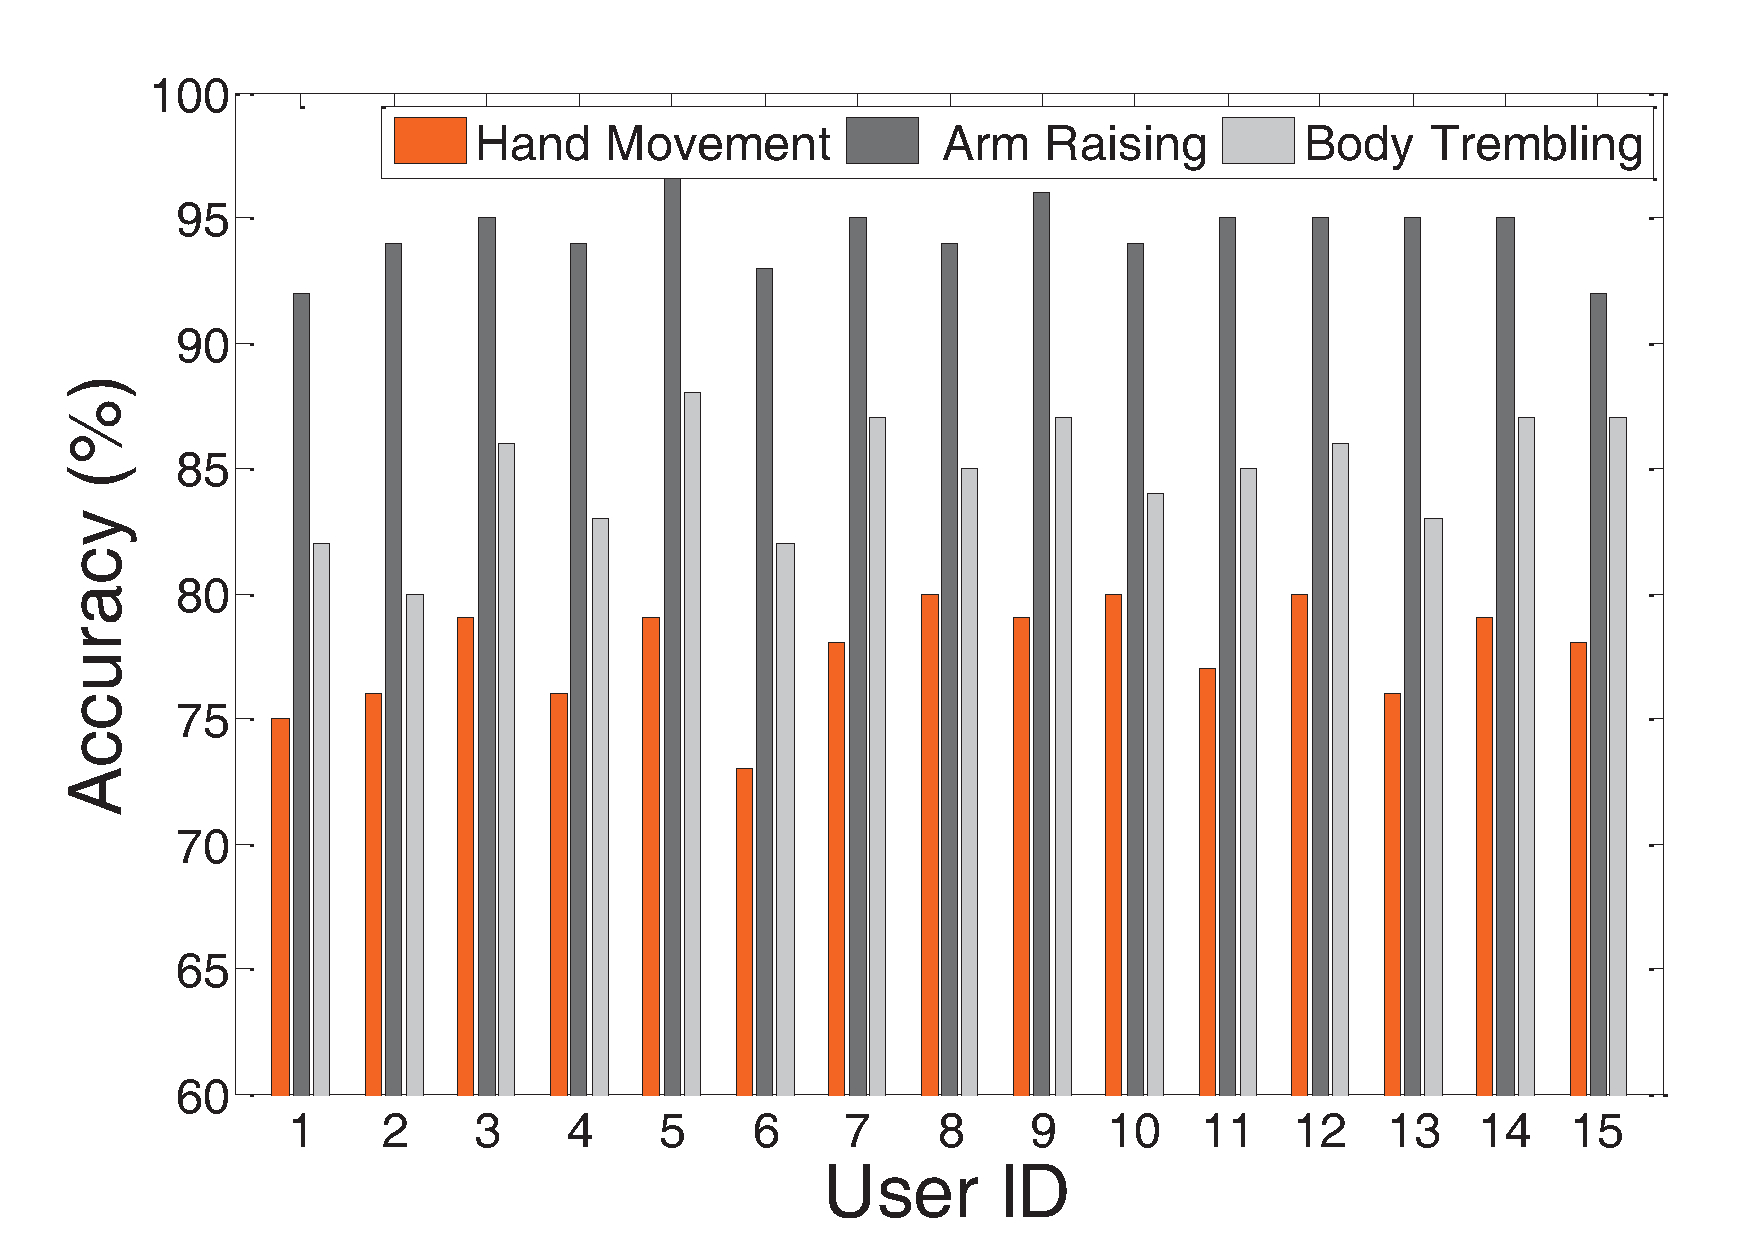
\includegraphics[width=6.5cm,height=4.7cm]{Figures/micro_movement_zhu.pdf}
		\caption{Detection accuracy of micro body movement.}\label{fig:micro_movement_zhu}	
	\end{minipage}%
	\begin{minipage}{.5\textwidth}
	 \centering
	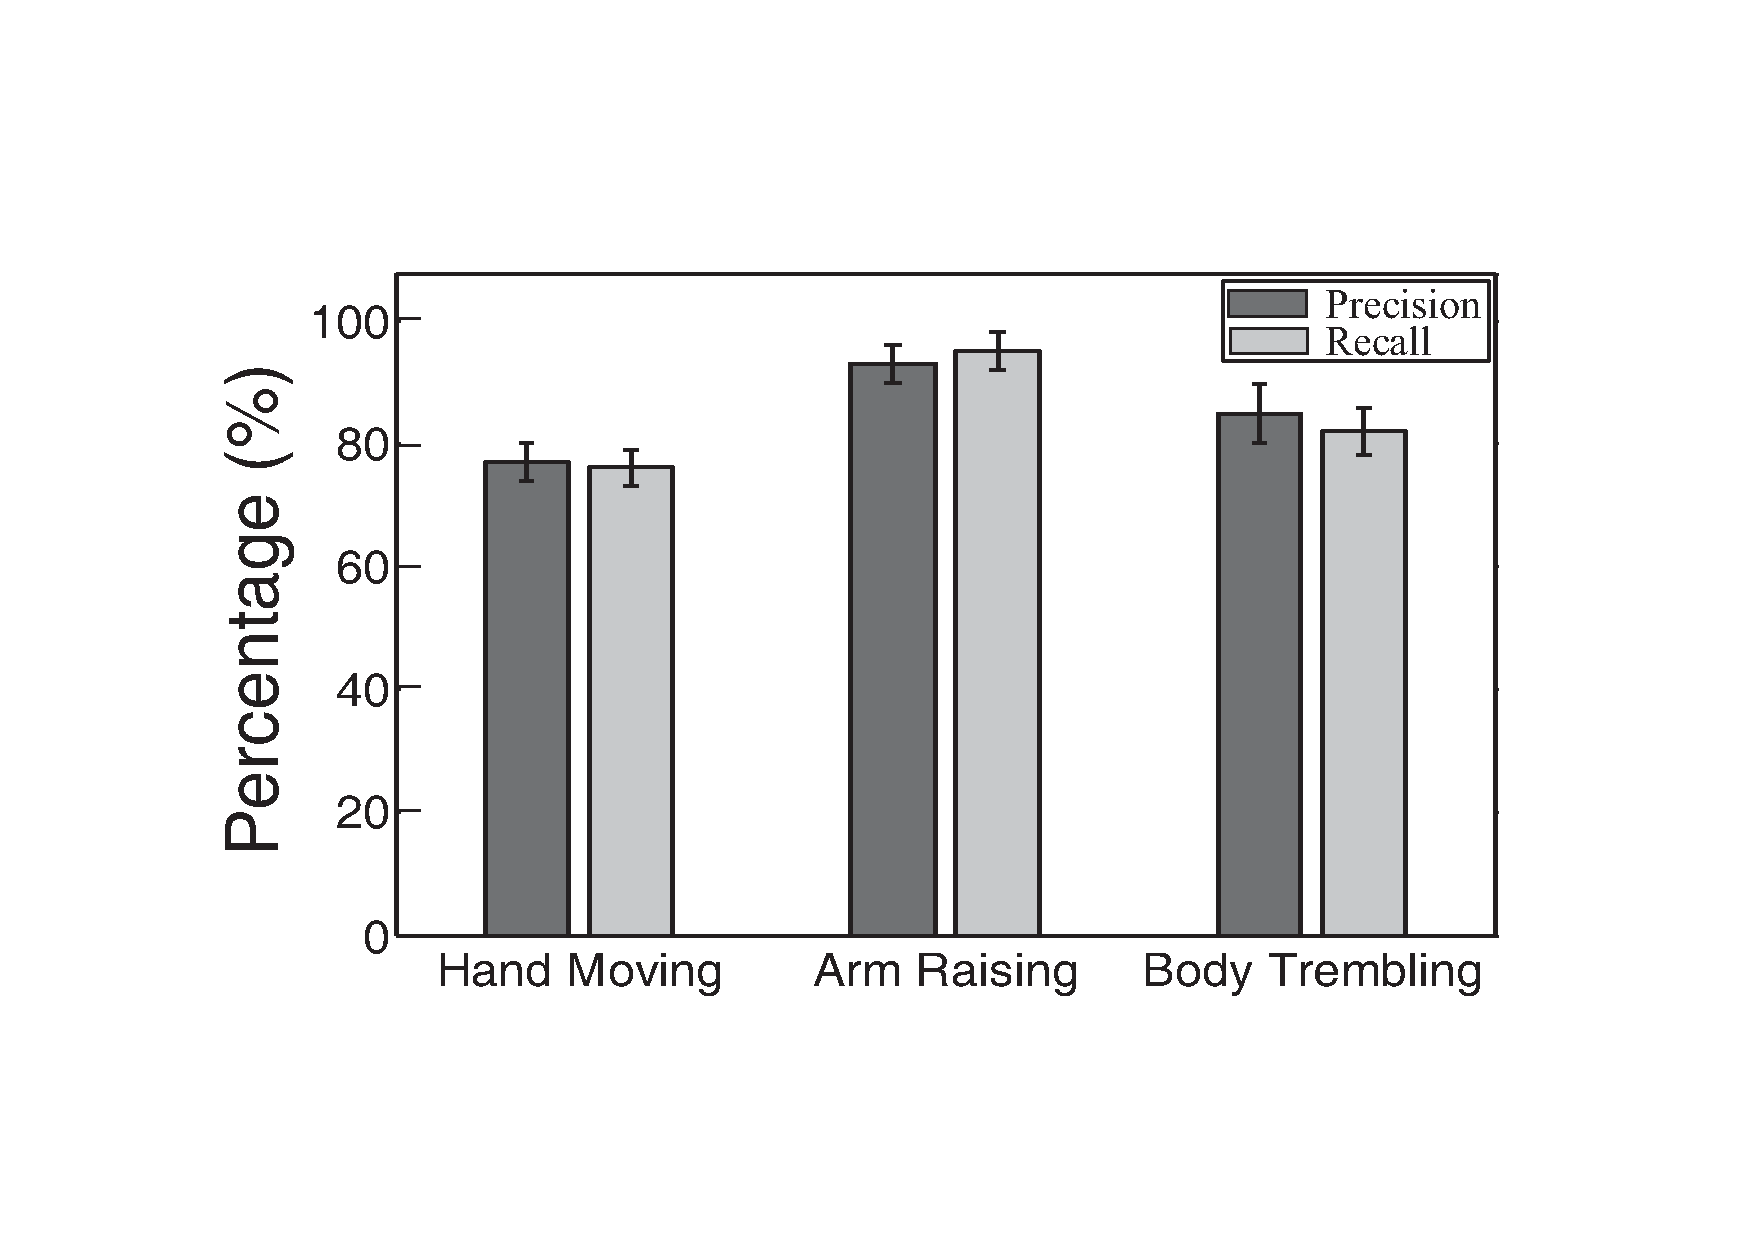
\includegraphics[width=6.5cm,height=4.7cm]{Figures/micro_combine1.pdf}
	\caption{Performance of micro body movement detection.}\label{fig:micro_combine}
	\end{minipage}
\end{figure}



 \subsubsection{Performance of acoustic events detection}
To study the detection accuracies of different acoustic events, we compare the ground truth recorded by the camera with the detected results by our system. Table \ref{tab:sound} shows the results across 15 participants. We can see that the precision for cough event is 88.9\% and a little than other three events. The reason is that different user's cough patterns are different, the pre-defined parameters in the detection model does not include all possible patterns. \textcolor{blue}{For example, some people have a fast and continuous pattern of coughing, while others have a slower intermittent pattern.} In fact, we train these parameters, namely the "interval", "duration" and "frequency" of acoustic events, with only 120 sets of nighttime sound data. Those data come from 40 (21 males and 19 females) volunteers of different ages (from 15 to 60 years old) who are prone to snoring, coughing, or somniloquy at night. To further improve the detection accuracy, we can train particular parameters for different users. \textcolor{blue}{And we can further expand the training data to include more possible patterns, and can also make reasonable estimates of the possible patterns to refine the range of parameters and thus increase the accuracy.}


\begin{table}[!thbp]\footnotesize
% \tabcolsep1pt
  \centering  % ������
 \renewcommand\arraystretch{0.3}
  \caption{The confusion matrix of acoustic events detection.}\label{tab:sound}
\begin{tabular}{c| c | c | c | c | c | c}
   \hline
   &\multicolumn{1}{ c|}{ }
   & \multicolumn{4}{ c|}{ }\\
   \multirow{2}*{}
&\multicolumn{1}{c|}{\multirow{2}*{{ Result}}}
&\multicolumn{4}{c|}{{ Prediction}}
& \multirow{4}*{{ Recall}} \\
    %&\multicolumn{5}{ c |}{\textbf{\small Prediction}} \\
   % & \multicolumn{5}{ c |}{ } \\
    \cline{3-6}
    & & & & & \\
    \multicolumn{1}{c|}{{}}
    &  \multicolumn{1}{c|}{{}}
    &  \multicolumn{1}{c|}{{ Snore}}
    &  \multicolumn{1}{c|}{{ Cough}}
    &  \multicolumn{1}{c|}{{ Somniloquy}}
    &  \multicolumn{1}{c|}{{ Other}}   \\
    & & & & & \\
     \cline{1-7}
    & & & & & \\
    \multirow{5}{*}{\begin{sideways}{{ Groundtruth}}\end{sideways}}
    &   { Snore}   & {\bf{{96}}}    &   $0$      &   $0$      &   $9$    &   {91.4\%}\\
    & & & & & \\
    \cline{2-7}
    & & & & & \\
   &   { Cough}   &   $3$      &   {\bf{{64}}}     &   $0$      &   $4$   &   {90.1\%} \\
    & & & & & \\
     \cline{2-7}
    & & & & & \\
    &   { Somniloquy}   &   $0$      &   $3$      &  {\bf{{42}}}      &   $2$  &   {89.4\%}  \\
    & & & & & \\
     \cline{2-7}
    & & & & & \\
    &   { Other}   &   $0$      &   $5$      &   $4$      &   {\bf{{325}}}   &   {97.3\%} \\
    & & & & & \\
    \hline
    & & & & & \\
    &   { Precision}      &   {96.9\%}   &   {88.9\%}   &   {91.3\%}   &   {95.6\%}    \\
    & & & & & \\
    \hline
   \end{tabular}
\end{table}


\subsection{Overall performance}

\subsubsection{Performance of sleep stage detection}

In order to prove that the detected events not only reflect the user's sleep habits, but also effectively identify the sleep stages to assess the sleep quality, we regard the reported results from Fitbit Charge2 as the ground truth. There are 50 sets of nocturnal sleep data selected from 210 sets of sleep data, \textcolor{blue}{in order to effectively assess performance while also reducing the time cost of the assessment. And to make the selection fairly and avoid overfitting,} we randomly pick at least 3 sets of data for each participant. For reflecting the sleep stage change carefully, \textcolor{blue}{{\systemname} use event-driven detection. When there is no sleep event detected in 15 minutes, we evaluates the sleep stage. When an event occurs, we immediately evaluates the sleep stage and use this time as the starting point for the next 15 minutes.} The averaged precision value and recall value are shown in Table \ref{tab:sleep stage}. It indicates that though {\systemname} may make misjudgement between the light sleep and REM, the overall performance is satisfying.

\begin{table}[!thbp]\footnotesize
%	\tabcolsep1pt
	\centering  % ������
	\renewcommand\arraystretch{0.4}
	\caption{{The confusion matrix of sleep stage detection.}}\label{tab:sleep stage}
	\begin{tabular}{c| c | c | c | c | c}
		\hline
		&\multicolumn{1}{ c|}{ }
		& \multicolumn{3}{ c|}{ }\\
		\multirow{2}*{}
		&\multicolumn{1}{c|}{\multirow{2}*{{ Result}}}
		&\multicolumn{3}{c|}{{ Prediction}}
		& \multirow{3}*{{ Recall}} \\
		%&\multicolumn{5}{ c |}{\textbf{\small Prediction}} \\
		% & \multicolumn{5}{ c |}{ } \\
		\cline{3-5}
		& & & & & \\
		\multicolumn{1}{c|}{{}}
		&  \multicolumn{1}{c|}{{}}
		&  \multicolumn{1}{c|}{{ REM}}
		&  \multicolumn{1}{c|}{{ Light Sleep}}
		&  \multicolumn{1}{c|}{{ Deep Sleep}} \\
	%	& & & & & \\
		\cline{1-6}
		& & & & & \\
		\multirow{1}{*}{\begin{sideways}{{ Groundtruth}}\end{sideways}}
		&   { REM}   & {\bf{{476}}}    &   $143$      &   $61$     &   {70.0\%}\\
		& & & & & \\
		\cline{2-6}
		& & & & & \\
		&   { Light Sleep}   &   $131$      &   {\bf{{508}}}     &   $91$      &   {69.6\%} \\
		& & & & & \\
		\cline{2-6}
		& & & & & \\
		&   { Deep Sleep}   &   $63$      &   $113$      &  {\bf{{262}}}      &   {59.8\%}  \\
		& & & & & \\
		\cline{1-6}
		& & & & & \\
		&   { Precision}      &   {71.0\%}   &   {66.5\%}   &   {63.3\%}   \\
		& & & & & \\
		\hline
	\end{tabular}
\end{table}

\subsubsection{Effect of respiratory amplitude on sleep stage detection}
When we detect different sleep stages, we also consider the respiratory amplitude when the hand's position is in the abdomen or chest. To assess the effectiveness of respiration amplitude estimation, we evaluate the performance of the sleep stage detection in two cases, that are with and without taking the respiration amplitude into account. The performance of sleep stage detection is shown in Table \ref{tab:respiratory}. For three different sleep stages, both the precision and recall values are improved with the help of respiration amplitude estimation. \textcolor{blue}{In fact, respiratory frequency can also be used as a feature to help us to detect sleep stages. But in fact  their essence the same. The difference in respiratory amplitude will also affect the difference in respiratory frequency, because when the respiratory amplitude is large, the time taken for one breath will be long, and the frequency of breathing will be slower. In {\systemname}, we choose the respiratory amplitude because the feature is very intuitive.}

\begin{table}[!thbp]\footnotesize
	\centering  % ������
	\renewcommand\arraystretch{0.3}
	\caption{Effect of respiration amplitude estimation.}\label{tab:respiratory}
	\begin{tabular}{c| c | c | c | c | c | c| c |}
		\cline{2-8}
		&\multicolumn{1}{ c|}{ }
		&\multicolumn{2}{ c|}{ }
		&\multicolumn{2}{ c|}{ }
		& \multicolumn{2}{ c|}{ }\\
		%  \multirow{4}*{}
		&\multicolumn{1}{c|}{}
		&\multicolumn{2}{c|}{\textbf{\footnotesize REM}}
		&\multicolumn{2}{c|}{\textbf{\footnotesize Light Sleep}}
		&\multicolumn{2}{c|}{\textbf{\footnotesize Deep Sleep}} \\
		%&\multicolumn{5}{ c |}{\textbf{\small Prediction}} \\
		% & \multicolumn{5}{ c |}{ } \\
		\cline{2-8}
		& & & & & & &\\
		\multicolumn{1}{c|}{\textbf{}}
		&  \multicolumn{1}{c|}{\textbf{Features}}
		&  \multicolumn{1}{c|}{\footnotesize Precision}
		&  \multicolumn{1}{c|}{\footnotesize Recall}
		&  \multicolumn{1}{c|}{\footnotesize Precision}
		&  \multicolumn{1}{c|}{\footnotesize Recall}
		&  \multicolumn{1}{c|}{\footnotesize Precision}
		&  \multicolumn{1}{c|}{\footnotesize Recall}\\
		& & & & & & &\\
		\cline{2-8}
		& & & & & & &\\
		\multirow{5}{*}
		&   \textbf{\footnotesize Without Respiration Amplitude}   & $62.9\%$    &   $63.4\%$      &   $59.4\%$      &   $63.9\%$    &   $57.7\%$ &  $54.1\%$ \\
		& & & & & & &\\
		\cline{2-8}
		& & & & & & &\\
		&   \textbf{\footnotesize With Respiration Amplitude}   &   $71.0\%$      &   $70.0\%$     &   $66.5\%$      &   $69.7\%$   &   $63.3\%$ &   $59.8\%$ \\
		& & & & & & &\\
		
		\cline{2-8}
		
	\end{tabular}
\end{table}

\subsubsection{Performance comparison}
We compare {\systemname} with two state-of-the-art work, the sleep detection app Sleep As Android and smartphone-based system Sleep Hunter \cite{gu2016sleep}.  Considering that Sleep As Android can only detect light sleep stage and deep sleep stage, we only compare the performance of these two stages. Table \ref{tab:comparison} shows the detection results.
As we can see, {\systemname}  performs much better than Sleep As Android and slightly better than Sleep Hunter. This good performance comes from the incorporation of rich and complicated sleep events. Therefore, our system helps users understand their sleep more easily and improve  sleep quality more effectively.

  \begin{table}[!thbp]\footnotesize
 	\centering  % ������
 	\renewcommand\arraystretch{0.3}
 	\caption{Performance of sleep stage detection comparison.}\label{tab:comparison}
 	\begin{tabular}{c| c | c | c | c | c |}
 		\cline{2-6}
 		&\multicolumn{1}{ c|}{ }
 		&\multicolumn{2}{ c|}{ }
 		&\multicolumn{2}{ c|}{ }\\
 		%  \multirow{4}*{}
 		&\multicolumn{1}{c|}{}
 		&\multicolumn{2}{c|}{\textbf{\footnotesize Light Sleep}}
 		&\multicolumn{2}{c|}{\textbf{\footnotesize Deep Sleep}} \\
 		%&\multicolumn{5}{ c |}{\textbf{\small Prediction}} \\
 		% & \multicolumn{5}{ c |}{ } \\
 		\cline{2-6}
 		\multicolumn{1}{c|}{\textbf{}}
 		&  \multicolumn{1}{c|}{\diagbox{System}{Stage}}
 		&  \multicolumn{1}{c|}{\footnotesize Precision}
 		&  \multicolumn{1}{c|}{\footnotesize Recall}
 		&  \multicolumn{1}{c|}{\footnotesize Precision}
 		&  \multicolumn{1}{c|}{\footnotesize Recall}\\
 		\cline{2-6}
 		& & & & & \\
 	%	\multirow{3}{*}
 		&   \textbf{\footnotesize SleepGuard}   & $66.5\%$    &   $69.6\%$      &   $63.3\%$      &   $59.8\%$  \\
 		& & & & &  \\
 		\cline{2-6}
 		& & & & & \\
 		&   \textbf{\footnotesize Sleep As Android}   &   $27.8\%$      &   $35.4\%$     &   $35.7\%$      &   $50.2\%$   \\
 		& & & & &  \\
 		\cline{2-6}
 		& & & & & \\
 		&   \textbf{\footnotesize Sleep Hunter}   &   $66.74\%$      &   $66.11\%$     &   $60.00\%$      &   $50.73\%$   \\
 		& & & & &  \\
 		
 		\cline{2-6}
 		
 	\end{tabular}
 \end{table}


Further, we compare {\systemname}'s functions with 8 other sleep detection products  in Table \ref{tab:function}, including Sleep As Android, Sleep Hunter, sleepMonitor \cite{sleepmonitor}, Sleeptracker \cite{sleeptracker}, Fitbit, isleep \cite{hao2013isleep}, Jawbone \cite{Jawbone} and ubiSleep \cite{pombo2016ubisleep}.  {\systemname} detects a wider range of sleep events and thus provides a better user experience.

\begin{table*}[!thbp]\footnotesize
%\setlength{\abovecaptionskip}{0.8pt}
  \centering  % ������
  \tabcolsep7pt
  %\arrayrulewidth1pt
  \caption{Functions comparision between different systems.}\label{tab:function}
  \renewcommand{\multirowsetup}{\centering}
  \noindent\makebox[\textwidth]{%
        \begin{tabularx}{1.0\textwidth}{|c|c|c|c|c|c|c|}
        \cline{1-7}
        \multicolumn{1}{|c|}{\multirow{2}*{\textbf{\footnotesize System}}}
        &\multicolumn{6}{c|}{\textbf{ \footnotesize Detected Events}} \\
         \cline{2-7}
    &  \multicolumn{1}{c|}{\textbf{ \footnotesize Heart Rate }}
    &  \multicolumn{1}{c|}{\textbf{ \footnotesize Acoustic Event }}
    &  \multicolumn{1}{c|}{\textbf{ \footnotesize Sleep Posture }}
     &  \multicolumn{1}{c|}{\textbf{ \footnotesize Body Movement }}
      &  \multicolumn{1}{c|}{\textbf{ \footnotesize Hand Position}}
       &  \multicolumn{1}{c|}{\textbf{ \footnotesize Sleep Stage}} \\
        \cline{1-7}
        \multirow{7}{2.14cm}
        {\textbf{SleepGuard\\Sleep as Android\\Sleep Hunter\\SleepMonitor\\Sleeptracker\\isleep \\Fitbit\\Jawbone\\ ubiSleep } }
        & &$\checkmark$ & $\checkmark$ &  $\checkmark$  &$\checkmark$ &$\checkmark$\\
        & &$\checkmark$ & & & &$\checkmark$\\
        & & $\checkmark$& &$\checkmark$ & &$\checkmark$\\
        & & & $\checkmark$ & & &\\
        &$\checkmark$ & & & & &$\checkmark$\\
         & &$\checkmark$ &   &$\checkmark$ & &\\
         &$\checkmark$ & & & & &$\checkmark$ \\
        & & & & & &$\checkmark$ \\
        & $\checkmark$&$\checkmark$ & & & &\\
        \cline{1-7}
 \end{tabularx}}
\end{table*}

\subsubsection{User survey}
\textcolor{blue}{In order to understand and verify whether the events detected by SLEEPGUARD are really interested or needed by users, we investigated and researched users. The user survey we conducted consisted of two types of people. One is the 15 volunteers who participated in our experiment, we not only conducted a sleep quality assessment for them but also investigated these users�� experience for SLEEPGUARD. And the others do not use our system, so, they only be asked if they were interested in or recognized the events we detected. Therefore, the results of the user survey are also composed of two parts. They are the assessment of sleep quality and the survey of user experience.For the assessment of sleep quality, we asked participants to fill out our questionnaire based on PSQI [16] every morning during the experiments, and compare the results of SLEEPGUARD and Fitbit
measurements with it. The questions in our survey include:}
\begin{enumerate}
  \item Subjective sleep quality (5 levels, 1 for excellent and 5 for worst),
  \item Sleep duration,
  \item Sleep disturbances,
  \item Daytime dysfunction.
\end{enumerate}
For the above four items, each one is rated on a 1 to 5 scale. These scores are first summed to yield a total score, which ranges from 0 to 20. Then we merge every five neighboring scores into one scale and eventually divide the total scores into four levels, recorded as 0, 1, 2 and 3, representing poor, general, good and excellent, respectively. The final sleep quality score comes from the comprehensive scores of above four questionnaires.

\textcolor{blue}{The 14-days averagesleep quality scores from 15 participates are presented in Table \ref{tab:quality}. We also list the sleep quality results obtained from SLEEPGUARD and Fitbit. In Table \ref{tab:quality}, as we can see, these value are the 14-day average results obtained by combining the sleep quality scores for each participant per day. The scores are divided into four levels, recorded as 0, 1, 2 and 3, representing poor, general, good and excellent, respectively. We compared sleep quality scores from {\systemname}, Fitbit, and user surveys. We can see that although {\systemname}'s assessment of sleep quality scores is only consistent with 9 users' subjective feelings. and only slightly better than Fitbit's results.However, results of the {\systemname} assessment are similar to those of the user survey. Possible inconsistencies are scores 2 and 3, that is, good and excellent, score 0 and 1, that is, poor and general, and there are few cases in which bad sleep has been assessed as good. These similar results are acceptable. We also found that when the results of the {\systemname} were inconsistent with the results of the user survey, it was consistent with the Fitbit results. The reason for such a situation may be that, for example, the user feels good about his own sleep but actually still has some neglected problems during sleep, which is detected by the sleep detection device, which is very helpful to the user. So we can find through the user survey these sleep behaviour we detected are indeed effective and beneficial for people, especially for users with sleep problems.}

\textcolor{blue}{In addition, we summarized the sleep problems and habit of the 15 volunteers who participated in our system assessment through a questionnaire survey and quality of sleep assessment. Then we found that there is a participant reported that his arm was always paralyzed, and five participants had poor sleep quality. We can find that the reason why the user's arm is numb is his incorrect sleep habits. The results from {\systemname} showed that he always tends to put his hands on his head, and long-term postures like this will inevitably lead to numbness of the arms. For similar situations, we will inform and remind users of their inappropriate postures and habits, and recommend that users should take measures to improve such situations. And for the poor quality of sleep of users, we analyzed the cause one by one based on events detected by {\systemname}. Through {\systemname}'s detecting, one user showed obvious symptoms of the difficulty of falling asleep and an unusually high number of body rollover. Our further analysis revealed that there was excessive light intensity and frequent noise in his sleeping environment. This may have led to the appearance of these symptoms and thus the poor quality of sleep. Then {\systemname} will recommend that users should focus on and improve his sleeping environment. In fact, this situation is very common that some users often choose to sleeping with a bright light because of one's fear of going to sleep alone. Even if they can also feel that this has an impact on their sleep. But in fact doing so for a long time is very bad for sleep and health. So {\systemname} also gives some suggestions for resolution, for example, do some proper exercise before going to bed or go to sleep with soft music that can be automatically turned off. And there is a user reported that he always had a nightmare at night, which led to poor sleep quality. We analyse the results of {\systemname} and found that user has been accustomed to sleep in the left side, and sometimes the hand is habitually placed on the chest. As \cite{nightmare} points that people who sleep on their left side are more at risk of nightmares. And the oppression of the chest by the hand causes the brain to have an ill hallucination, making it extremely easy to make a nightmare. So {\systemname} suggest to the user based on these two possible reasons, and hope that the user can take some special measures to change it, and recommend that the user can take some additional methods, such as listening to some soothing music to relax before sleep. Another user was detected by {\systemname} to be bothered by long-term snoring, as he himself mentioned. We know that the occurrence of snoring is most likely due to improper sleeping posture, and we also detected that the user is accustomed to sleep in a supine position, so on the one hand, {\systemname} suggests that the user try the sleeping position in the side position. On the other hand, if the situation still does not improve very well, it is recommended that the user go to the hospital in time for a corresponding check to avoid snoring caused by certain diseases. In addition, if we detect that some users are accustomed to sleeping in a prone position, we will remind and advise them because the prone position is bad for health.}

\textcolor{blue}{According to different possible reasons, {\systemname} proposes different reminders and suggestions to users, such as adjusting their sleeping posture, improving the sleeping environment, and consciously avoiding bad sleeping habits. As for how to adjust and avoid them, users can take special, mandatory or medical methods according to their own situation. For example, \cite{posture} present an anti-supine device mimicking the so-called "tennis ball technique" to control sleep posture, in order to improve OSA hypopnoea syndrome. And it is recommended that long-term snoring users perform physical examination so that they can timely The discovery of physical diseases that is most likely to cause snoring such as high blood pressure, cardiovascular and cerebrovascular diseases. In addition, we asked the 15 participants to make appropriate adjustments according to our recommendations and to conduct a return visit survey three weeks later. It was found that some of the users had some symptoms relieved and the average quality of sleep was improved.}
	
\textcolor{blue}{As for the user experience, we can find that most people are praised and interested in these events detected by {\systemname}.} 80\% of participants believe that the detection of sleep posture is very necessary, showing their sleep posture can not only help people to avoid health problems caused by long-term improper sleeping posture, but also help us find out the reasons for the next day's physical discomfort, such as dizziness, muscle soreness may be due to improper sleeping posture. \textcolor{blue}{And there are some users are troubled by snoring. This may be due to improper sleeping posture. We map the detected snoring event and sleeping posture to suggest the user to modify his posture to a suitable posture to reduce the harm caused by long-term snoring.} 60\% of the participants thought it useful to detect the hand position in supine posture, even one user mentioned that he did often have nightmares and our system found his hand was often placed on his chest, and then {\systemname} could remind him that he should take some measures to avoid such a position and thus reduce the poor sleep quality that nightmare brings. Only 20\% of participants found it useful to calculate the number of body rollover. However, detection of rollovers is useful in segmenting sleep stages. Furthermore, body rollover counts could be used to derive additional information to the user, such as how restless or peaceful the sleep has been overall.


\begin{table} \footnotesize
  \centering  % ������
  \renewcommand\arraystretch{0.5}
  \caption{Results of sleep quality assessment.}\label{tab:quality}
\begin{tabular}{c| c | c | c | c | c |c |c |c |c |c| c |c |c |c |c |c |c|}
   %\cline{2-6}
   %&\multicolumn{1}{ c|}{ }
   %&\multicolumn{2}{ c|}{ }
  % &\multicolumn{2}{ c|}{ }\
    %&\multicolumn{1}{c|}{}
   %&\multicolumn{2}{c|}{\textbf{\scriptsize Light Sleep}}
  % &\multicolumn{2}{c|}{\textbf{\scriptsize Deep Sleep}} \\
    %&\multicolumn{5}{ c |}{\textbf{\small Prediction}} \\
   % & \multicolumn{5}{ c |}{ } \\
    \cline{2-17}
    \multicolumn{1}{c|}{\textbf{}}
    &  \multicolumn{1}{c|}{\diagbox{System}{User ID}}
    &  \multicolumn{1}{c|}{\footnotesize  1}
    &  \multicolumn{1}{c|}{\footnotesize  2}
    &  \multicolumn{1}{c|}{\footnotesize  3}
    &  \multicolumn{1}{c|}{\footnotesize  4}
    &  \multicolumn{1}{c|}{\footnotesize  5}
    &  \multicolumn{1}{c|}{\footnotesize  6}
    &  \multicolumn{1}{c|}{\footnotesize  7}
    &  \multicolumn{1}{c|}{\footnotesize  8}
    &  \multicolumn{1}{c|}{\footnotesize  9}
    &  \multicolumn{1}{c|}{\footnotesize  10}
    &  \multicolumn{1}{c|}{\footnotesize  11}
    &  \multicolumn{1}{c|}{\footnotesize  12}
    &  \multicolumn{1}{c|}{\footnotesize  13}
    &  \multicolumn{1}{c|}{\footnotesize  14}
    &  \multicolumn{1}{c|}{\footnotesize  15}\\
     \cline{2-17}
    & & & & & & & & & & & & & & & & \\
    \multirow{16}{*}
    &   \textbf{\footnotesize SleepGuard}  & $3$ & $3$ & $0$ & $1$ & $2$ & $2$ & $3$ & $0$ & $2$ & $2$ & $2$ & $2$ & $1$ & $0$ & $2$ \\
   & & & & & & & & & & & & & & & &\\
    \cline{2-17}
   & & & & & & & & & & & & & & & &\\
   &   \textbf{\footnotesize Fitbit}   & $3$ & $3$ & $0$ & $0$ & $1$ & $3$ & $2$ & $3$ & $2$ & $2$ & $2$ & $2$ & $2$ & $1$ & $2$\\
      & & & & & & & & & & & & & & & & \\
      \cline{2-17}
       & & & & & & & & & & & & & & & & \\
    &   \textbf{\footnotesize User survey}  & $3$ & $2$ & $0$ & $0$ & $2$ & $2$ & $3$ & $1$ & $1$ & $2$ & $2$ & $3$ & $0$ & $0$ & $2$ \\
     & & & & & & & & & & & & & & & & \\
    \cline{2-17}
   \end{tabular}
\end{table}

%\begin{figure}
 %\centering
% 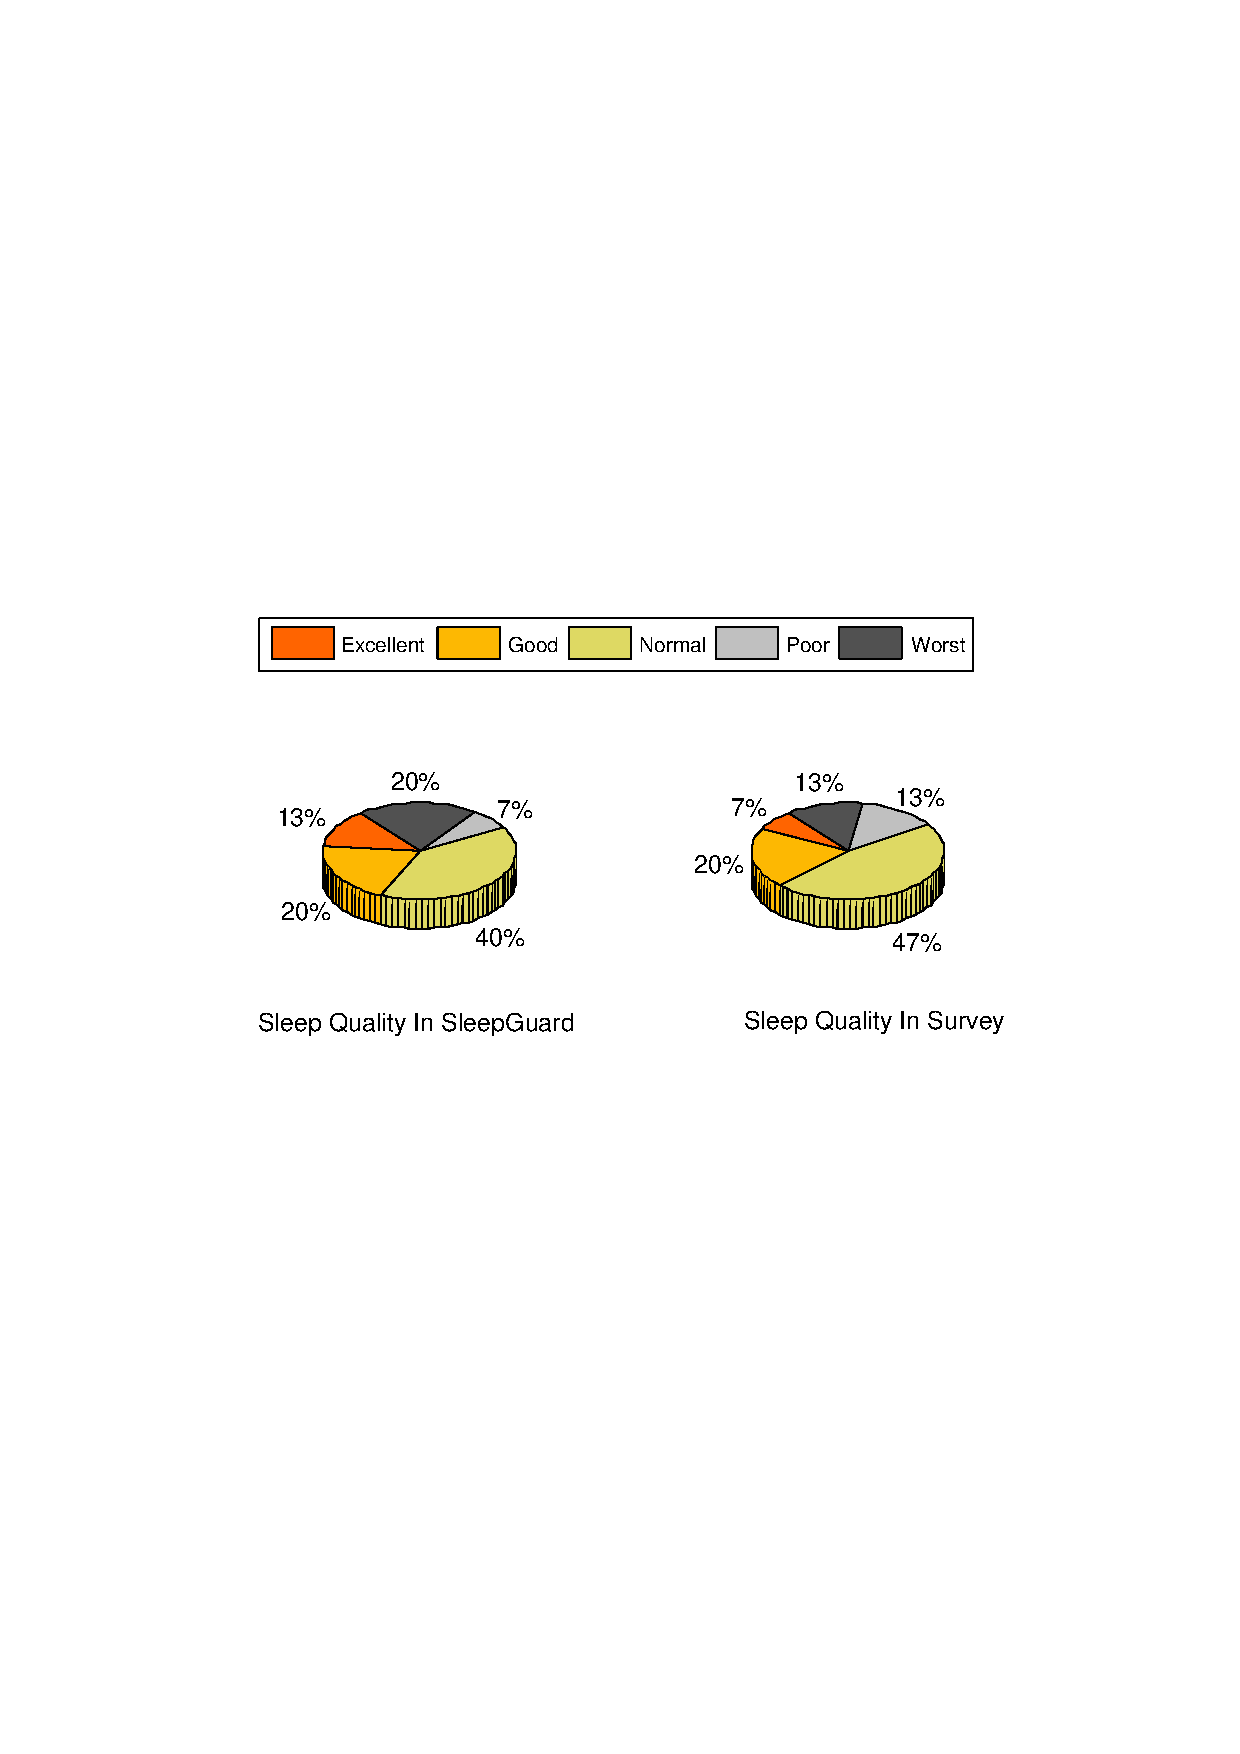
\includegraphics[width=0.52\linewidth]{Figures/quality.pdf}
 %\caption{Participants' sleep quality distribution}\label{fig:quality}
%\end{figure}

\section{DISCUSSION}\label{sec:discussion}

In this paper, we have shown that sensors available on off-the-shelf smartwatches can be used to capture rich information about sleep quality and factors affecting it. The main focus of our work has been to develop the required algorithms for capturing rich sleep related information as accurately as possible. While the recognition performance of our system is very encouraging, there are some issues that would need to be addressed in our system before larger-scale deployment would be feasible. Below we highlight the main issues and briefly discuss possible ways to overcome them.


%In this work, we try to examine the possibilities of using smart wearables to detect sleep. Our focus is to provide a series of ways to detect sleep-related events that will greatly assist in the assessment of sleep quality.While our results are satisfactory, there are still a handful of issues to address as we highlight below.

\begin{itemize}
  \item \textbf{The accuracy of sleep stage detection.}
  Compared with polysomnography-based sleep stage detection, the accuracy of {\systemname} is lower and it is rather difficult to achieve comparable performance. This is because polysomnography monitors and analyzes sleep based on information that directly correlates with sleep such as EEG, EMG, EOG, and oxygen saturation, whereas {\systemname} estimates sleep quality from cues that have an indirect effect on sleep quality. In particular, \systemname only combines the body movement, acoustic events, sleep environment and other events during sleep to predict the sleep stage. Therefore, {\systemname} is not a replacement for professional medical equipment for high-precision sleep detection, but serves as a personal technology that provides easy-to-use and non-intrusive way to monitor personal sleep patterns and to obtain feedback about the sleep quality. Moreover, it can trace back to the real causes affecting sleep quality, and guide users to have the direction to improve sleep quality.% However, SleepGuard is able to take advantage of the popularity of business smartwatches to provide easy-to-use and less intrusive sleep detection services, making it easy for users to learn about their sleep and make adjustments based on suggestions.
  \item \textbf{Battery life.}
  A critical design requirement for sleep detection is that the monitoring can operate sufficiently long to cover the entire duration of the user's sleep. Battery capacity on smartwatches is rather limited, resource consumption needs to be optimized by considering both the data collection and analysis phases. In our experiments we demonstrated that additional devices in the vicinity of the smartwatch can be taken advantage of, for example, some of the sensing and processing tasks can be offloaded to smartphones or other smart devices located within sufficient proximity. Particularly the acoustic event detection could be offloaded to smartphones that are located on the bedside table or elsewhere in the user's vicinity as smartphones increasingly integrate co-processors for audio processing that allow performing the audio event detection with a small energy footprint. We have also designed our analysis techniques to be as lightweight as possible to minimize energy consumption. Further improvements can be achieved by designing dynamic duty cycling strategies that reduce sampling during periods of regularity, and by using simple triggering mechanisms, such as a motion intensity detector to reduce processing overhead. Exploring these techniques is part of our future work.%For our work, we only use smartwatch as devices for data collection and delivery, while other computing capabilities are mainly implemented on smartphone, and we also have adopted simpler algorithms to reduce resource usage. But despite this, our smartwatch can only continue to collect about 6 hours of sensor data, which is not sufficient for longer sleep detection, so we still need to further study how to reduce power consumption. One possible solution is to change the data collection strategy to dynamically adjust the sampling frequency based on whether the body is moving or not.
  \item \textbf{Sensor data.}
  One limitation of {\systemname} is that we have not taken advantage of heart rate when determining the current sleep stage of the user. The main reason for this is programming limitations of the Huawai Smartwatch 2 device used in the experiments. Specifically, the device does not support querying heart rate information, but only provides it through a dedicated application. The output of this application is unfortunately not sufficiently accurate for sleep monitoring purposes, and restricts the rate at which information can be acquired. To compensate for the lack of heart rate data, \systemname considers the respiratory amplitude detected from accelerometer instead. As shown in our experiments, the respiratory amplitude detection significantly improves the performance of the sleep stage detection. % which can help us improve the performance of the sleep stage detection (it has been proved in our experiment).
  \item \textbf{Limitations of the algorithm.}
  When we try to detect sleep posture, we find a corresponding relationship between the position of the arm and the sleeping posture, so we indicate the sleeping posture by detecting its position. But currently we consider some specific positions of the arm in the four sleeping positions, some unusual arm's positions are ignored by us and that is something we need to improve further in future work.
  
  \item \textbf{Single wrist sensor.}
  In our paper, we only use the sensor data in the left-hand smart watch, though movement patterns of the left and right wrist are different during sleep, the technique used for detecting sleep related behaviors is the same. Some sleep related events like sleep posture, body rollover, acoustic events, illumination conditions, both of them are not affected by different wrists, the reason is that these events are related to the entire body rather than the part of the body. The only thing we need to do is adjusting new experimental parameters when the smartwatch is worn on different wrists. But for the hand position detection and body micro movement detection including the arm raising and hand movement does have an impact, it is because the hand movement probability and frequency are different on different hands. And the degree of impact on our detection performance varies from person to person and can be largely cancelled through calibration. This is where we need to measure and consider in our future work.
  
  In addition, when we use Fitbit as groundtruth, Fitbit is worn on a different wrist from {\systemname}. However, from the analysis of the basic principles of sleep stage detected by {\systemname} and Fitbit, it can be found that this does not have much effect on our assessment of the results. Both Fitbit and {\systemname} have common grounds for detecting sleep stages based on acoustic events, the occurrence and frequency of physical activity, but we go further to conduct more fine-grained detection and classification of these events, and add more consideration about illumination conditions and respiratory amplitude. One thing we can know is that the measurement of events such as acoustic events, body rollover events, body tremble, etc., has little to do with the sensor data collected from the left or right hand. The major difference that may exist is these rich events added in {\systemname}, such as hand position, sleep posture, etc,  but these are not detected by Fitbit, so they have no effect when compared. Moreover, we also did a test experiment. The smart watches were worn on the left and right hands respectively and the event detection algorithm in {\systemname} was mainly used to detect those events that are of concern in Fitbit. We can 19see that the results are not much different. Therefore, in the end, in order to ensure that the user��s sleep is as uncomfortable as possible, we choose to make Fitbit and Smartwatch are worn on different hands. 


  \item \textbf{Multiple sleepers}
  Currently, {\systemname} considers that the user is sleeping alone, but there are still more complicated situations in reality, such as sleeping with a bed partner, baby, and/or a pet. However, because {\systemname} is based on the detection of smartwatch, Unlike smartphone placed on the bed, it can show more sensitivity to the user's own activities. Therefore, for the detection performance of sleeping posture, body rollover and hand position events has almost no effect, but it may have some influence on the body micro movements and acoustic events. When people around us have relatively large movements, such as body rollover, they may fluctuate to users, making it possible for us to mistakenly detect it as user's micro movements. For this kind of situation, we can test the change of acceleration data in multi-sleeper situations by popularizing the experiment to adjust the detection threshold of our body's micro movements and achieve better detection performance. This will also be a direction for our future work. As for acoustic events, we can further limit conditions, such as training the different magnitudes of the energy of the sound signals collected by the user's hand at different positions to identify whether it is the user's own acoustic event or the sound of the bed partner. In addition, the related acoustic events of the bed partner can also be considered as a factor affecting the user's sleep.

  \item \textbf{Occurrence probability of unusual arm's positions.}
  We detect sleep posture based on arm's positions and focus on three specific positions when detecting the position of the hand. In sleep position detection, we are based on the assumption that between the user's arms position and sleeping postures that the arms have common and (reasonably) stable positions in each posture and we consider as many possible arm positions as possible in four sleeping postures, which are the most common arm's positions for users during sleep. In hand position detection, we chose the three most representative locations that do have an impact on sleep and health. But we know that not all users or a user will not have these common positions all the time. These unusual arm's positions may cause the performance of our sleep posture detection algorithm to degrade. But of the 15 participants we tested, we can see from the video that the unusual arm's positions are present, but these are basically a slight evolution of the common positions, which have little effect on the detection of the sleeping posture. Only a small part of the unusual position will cause us to produce false positives. For this issue, we will expand the test population to further measure the impact of unusual arm's position on our system and consider more hand positions in future work.

 \item \textbf{Actionable feedback.} The current version of {\systemname} has been designed to provide simple recommendations on how users should improve their sleeping environment and habits. These can be linked with additional suggestions that may alleviate the causes. For example, problems in falling asleep can be mitigated by doing some exercise before going to bed or by going to sleep with soft music that can be automatically turned off. Similarly, we can identify poor postures and hand positions and give feedback on what the users should aim to improve to reduce sleep problems. For example, \cite{posture} present an anti-supine device mimicking the so-called "tennis ball technique" to control sleep posture, in order to improve OSA hypopnoea syndrome.  For some problems, such as persistent snoring or coughing, our system can provide suggestions such as how to improve posture to mitigate these problems, or potentially detect severe cases where medical intervention would be appropriate. Indeed, for long term snoring the medical guidelines suggest undergoing a physical examination so that they can timely discover possible physical diseases that may cause snoring, such as high blood pressure, cardiovascular and cerebrovascular diseases. 

\end{itemize}

\section{RELATED WORK}\label{sec:5related}

Sleep quality is a crucial issue for each individual, and the poor sleep would lead to numerous diseases, such as  endocrine dyscrasia, depression, immunity decline \cite{vgontzas2009insomnia,gottlieb2005association}. Thus, a lot of research works have been proposed to monitor the sleep \cite{langkvist2012sleep,hao2013isleep,bai2012will,kay2012lullaby,bain2003evaluation,pombo2016ubisleep}. Below, we summarize the related state-of-the-art research works as the following three categories.

\textbf{Medical technology based work}. Traditionally, the dedicated medical technologies, like EEG, ECG and EMG \cite{saper2005hypothalamic}, have been applied for sleep monitoring. Those technologies rely on the certain biomedical signals, such as brain wave, muscle tone and eye movement, to assess the sleep quality. For example, the EEG technology in \cite{langkvist2012sleep,oropesa1999sleep,ebrahimi2008automatic} monitors the brain waves, and then recognizes the sleep stages by leveraging unsupervised learning approaches.

Although a high accuracy achieved by those  technologies, they have two drawbacks. First, those  technologies require the dedicated medical devices, which are very expensive compared the widely available  smart watch/phone. Second, they require the users to be attached lots of sensors on the human body, which may cause a healthy person had to sleep and result in large errors.

Compared with those medical technologies, our system has two advantages. First, we only need a smartwatch, which is cost effective. Second, the smartwatch does not disturb a user's normal sleep, thus we can monitor the user's sleep quality more accurately.

\textbf{Smartphone based work}. Recently, some researchers use the smartphones for sleep monitoring \cite{hao2013isleep,bai2012will,kay2012lullaby,choe2011opportunities} . iSleep \cite{hao2013isleep} measures the sleep quality by recording the sleep-related acoustic events and evaluates the sleep quality using the Pittsburgh Sleep Quality Index (PSQI) \cite{carpenter1998psychometric}. Bai et al. \cite{bai2012will} predicts a user's sleep quality by observing the user's daily activities with the smartphone's sensor data, like the accelerometer, gyroscope, microphone, etc. Work in \cite{kay2012lullaby} leverages the smartphone sensors to record the sleep disruptors for a user. The authors in \cite{choe2011opportunities}  explore a series of opportunities to support healthy sleep behaviors based on the smartphone sensors. Several research works predict the sleep quality by using the smartphone to monitor the external  influence  factors, such as the daily activity, sleeping environment, location and family settings \cite{chen2013unobtrusive,zhang2013real}. Besides those research works, many Smartphone Apps, such as Sleep As Android \cite{SleepAndroid}, Sleep Journal \cite{SleepJournal}, YawnLog \cite{YawnLog} also have been developed to monitor a uer's sleep quality.

Those smartphone based systems, however, require placing the smartphone at a specifically location near to the user, which usually cannot be satisfied in reality. For example, Gu et al. \cite{gu2016sleep} needs the smartphone to be placed next to the user's head, and requires the smartphone keeping stationary throughout the sleeping process. But, many users do not want to place the mobile phone too close to the body due to health risk concerns  \cite{StepHealth,Quorasleep}.

Compared with the existing smartphone based systems, our system uses the commodity smartwatch for sleep monitoring. Since many users are willing to wear the smartwatch throughout the night, thus the smartwatch can remain relatively close to the user over the duration of sleep so that more user-related data can be collected. \textcolor{blue}{And the performance of {\systemname} has been improved to some extent, but more advantages are reflected in the consideration of more abundant events, which enables a wider range of sleep-related events and more accurate to achieve sleep detection and sleep quality assessment.} %The smartwatch also allows us to collect a richer set of information, which enables a wider range of sleep-related events and more accurate to achieve sleep detection and sleep quality assessment.


\textbf{Wearable device based work}. With the widely use of wearable devices, more and more researchers and industries try to  use the smartwatch or wearable-wrist for sleep monitoring \cite{bain2003evaluation,bonnet2003insomnia,pombo2016ubisleep,caviness1996myoclonus}.  The Sleeptracker
\cite{sleeptracker} is a wristwatch-shaped unit that apart from telling the time, also infers whether the user is in deep sleep, light sleep, or awake, using an accelerometer. The ubiSleep \cite{pombo2016ubisleep} joints heart rate, accelerometer, and sound signals collected into the smartwatch for noninvasive sleep monitoring. The aXbo alarm clock [9] is packaged as a stand-alone application in the form of an alarm clock that wirelessly communicates with a wrist-band unit. The Zeo \cite{caviness1996myoclonus} is similarly using an alarm clock base unit with a worn sensing device, but the latter is a headband rather than a wrist-band that based on electroencephalograph (EEG) to monitor sleep. We know Zeo has good performance in sleep stage detection compared to some wristband sleep monitoring products because products based on some biological signals like EEG are able to get more accurate and more representative sleep data than actigraphy-based \cite{Actigraphy} sleep monitoring products. However, the vast majority of biosignal-based sleep detection approaches require specialized equipment, which is high cost and complex to operate, while the approaches based on actigraphy are well adapted and user-friendly to accept and understand.

Moreover, these actigraphy-based wristband devices or smartwatch Apps only can gather coarse-grained information and  do not design a model for deep understanding the relationship between a user's sleep pattern and the sensor data. For example, many smartwatch Apps, like Jawbone Up \cite{Jawbone}, FitBit \cite{fitbit}, YawnLog \cite{YawnLog} and WakeMate \cite{WakeMate}, do not show how they assess a user's sleep quality based on what kind of sensor data. \textcolor{blue}{In addition,  there is some work that uses wearable devices to detect certain detailed events of sleep. \cite{wear_related1}  design a cheap lowpower wrist-worn Sensors to monitor the user's sleep posture. \cite{wear_related2} detect roll-over and measure sleep quality using a wearable sensor. \cite{wear_related3} use a single chest-worn sensor to extract body acceleration and sleep position changes.}

\textcolor{blue}{Compared with the existing smartwatch or wearable-wrist based systems, our system is a more complete sleep monitoring system, and is based only on sensors in commercial smart watches without additional hardware. It collect an extensive set of sleep-related events, many of which are not supported in prior work. And for sleep monitoring in daily life, it is more practical and will not invasion users�� normal sleep , and more and more people are willing to accept to wear watches to fall asleep, unlike other wearable devices such as chest-worn sensors, most people are still unwilling to accept to wear her to sleep. Moreover, our original intention and focus are more inclined to enable users to have a deeper and more comprehensive understanding of their sleep, explore the causes of sleep quality, and provide users with more practical advice to point them in a clear direction for improving sleep quality and being healthy.}
%Compared with the existing smartwatch or wearable-wrist based systems, our system can collect an extensive set of sleep-related events, many of which are not supported in prior work. Our system enables users to gain a deeper understanding of their sleep patterns and the causes of poor sleep.

\textcolor{blue}{All in all, as we can see from Table \ref{tab:related_work}, the advantage of {\systemname} is that it can detect more fine-grained sleep-related events to obtain more abundant sleep information, which is currently on the market for commercial or scientific research sleep monitoring system can not be achieved. And the performance of {\systemname} has been improved to some extent. Our original intention and focus are more inclined to enable users to have a deeper and more comprehensive understanding of their sleep, explore the cause s of sleep quality, and provide users with more practical advice to point them in a clear direction for improving sleep quality and being healthy. And compared with some medical technology like PSG, our advantages are inexpensive and easy to deploy at home, so it is suitable for most general public. And it does not need a large number of instruments attached to the user's body, thus it has less intrusiveness for sleep and does not require professional personnel to operate. Although the accuracy of {\systemname}'s ability to detect sleep cannot be compared to medical technology, it is enough for the average family's daily sleep monitoring needs. The most important is that we concentrates on physical activities rather than biomedical signals, so these rich physical activities detected are easily understood by users, and they can be adjusted with improved and improved sleep based on the results of monitoring.}


\begin{table*}[!t]
  \centering
  \small
  \caption{Summary of existing solutions.}\label{tab:related_work}
        \begin{tabular}{lcccccc}
        \toprule
        \textbf{System} & \textbf{High accuracy} & \textbf{Practicality} & \textbf{Low disruptive} & \textbf{Low cost} & \textbf{Informativeness} & \textbf{Interpretability}  \\
        \midrule
        \rowcolor{Gray} PSG     &  $\checkmark$ & &  &   & $\checkmark$ &  \\

        Smartphone solutions& &$\checkmark$ &$\checkmark$  &$\checkmark$   & & $\checkmark$ \\

        \rowcolor{Gray} Wearable solutions& &$\checkmark$ & $\checkmark$ & $\checkmark$  & & $\checkmark$ \\
        \textbf{\systemname} & &$\checkmark$ &$\checkmark$  & $\checkmark$  & $\checkmark$&$\checkmark$  \\

        \bottomrule
  \end{tabular}
\end{table*}


\section{Summary and Conclusion}

In this paper, we have presented \systemname, the first holistic smartwatch-based sleep monitoring solution that can simultaneously estimate sleep quality and provide rich information about sleep events, including body motions, acoustic events related to sleep disorders, and ambient illumination. To capture this information accurately, we have proposed new algorithms for extracting the relevant events from sensor information. We demonstrated the benefits of \systemname through rigorous benchmark experiments carried out using measurements collected from a two week trial with $15$ participants. The results of our experiments demonstrate that \systemname provides comparable sleep quality estimation accuracy than state-of-the-art consumer grade sleep monitors, while at the same time being able to accurately capture a rich set of information about factors influencing sleep quality. This information is particularly important for identifying possible causes of poor quality sleep and can be used to provide the user with suggestions on how to improve their sleep quality, e.g., by improving their sleep environment or behaviours surrounding sleep. We also compared the sleep quality estimates of \systemname against subjective self assessments, demonstrating a high degree of correspondence. 

%This paper presents \systemname, a smartwatch based deep understanding of sleep detection system. \systemname exploits the rich sensor data
%provided by smartwatches to track a wider range of sleep-related activities. To detect sleep related activities, we effectively exploit the
%smartwatch sensor data and design a set of new algorithms based on the particular characteristics. Extensive experimental results show that
%\systemname can accurately identify lots of sleep activities, including body postures, body rollover, hand positions and acoustical events.
%In the future work, we will optimize the energy consumption and design detection models for more events.


\bibliographystyle{ACM-Reference-Format}
\bibliography{sleep_ref}

\end{document}
